% Options for packages loaded elsewhere
\PassOptionsToPackage{unicode}{hyperref}
\PassOptionsToPackage{hyphens}{url}
\PassOptionsToPackage{dvipsnames,svgnames,x11names}{xcolor}
%
\documentclass[
  a4paper,
  DIV=11]{scrreprt}

\usepackage{amsmath,amssymb}
\usepackage{iftex}
\ifPDFTeX
  \usepackage[T1]{fontenc}
  \usepackage[utf8]{inputenc}
  \usepackage{textcomp} % provide euro and other symbols
\else % if luatex or xetex
  \usepackage{unicode-math}
  \defaultfontfeatures{Scale=MatchLowercase}
  \defaultfontfeatures[\rmfamily]{Ligatures=TeX,Scale=1}
\fi
\usepackage{lmodern}
\ifPDFTeX\else  
    % xetex/luatex font selection
\fi
% Use upquote if available, for straight quotes in verbatim environments
\IfFileExists{upquote.sty}{\usepackage{upquote}}{}
\IfFileExists{microtype.sty}{% use microtype if available
  \usepackage[]{microtype}
  \UseMicrotypeSet[protrusion]{basicmath} % disable protrusion for tt fonts
}{}
\makeatletter
\@ifundefined{KOMAClassName}{% if non-KOMA class
  \IfFileExists{parskip.sty}{%
    \usepackage{parskip}
  }{% else
    \setlength{\parindent}{0pt}
    \setlength{\parskip}{6pt plus 2pt minus 1pt}}
}{% if KOMA class
  \KOMAoptions{parskip=half}}
\makeatother
\usepackage{xcolor}
\ifLuaTeX
  \usepackage{luacolor}
  \usepackage[soul]{lua-ul}
\else
  \usepackage{soul}
  
\fi
\setlength{\emergencystretch}{3em} % prevent overfull lines
\setcounter{secnumdepth}{5}
% Make \paragraph and \subparagraph free-standing
\ifx\paragraph\undefined\else
  \let\oldparagraph\paragraph
  \renewcommand{\paragraph}[1]{\oldparagraph{#1}\mbox{}}
\fi
\ifx\subparagraph\undefined\else
  \let\oldsubparagraph\subparagraph
  \renewcommand{\subparagraph}[1]{\oldsubparagraph{#1}\mbox{}}
\fi

\usepackage{color}
\usepackage{fancyvrb}
\newcommand{\VerbBar}{|}
\newcommand{\VERB}{\Verb[commandchars=\\\{\}]}
\DefineVerbatimEnvironment{Highlighting}{Verbatim}{commandchars=\\\{\}}
% Add ',fontsize=\small' for more characters per line
\usepackage{framed}
\definecolor{shadecolor}{RGB}{241,243,245}
\newenvironment{Shaded}{\begin{snugshade}}{\end{snugshade}}
\newcommand{\AlertTok}[1]{\textcolor[rgb]{0.68,0.00,0.00}{#1}}
\newcommand{\AnnotationTok}[1]{\textcolor[rgb]{0.37,0.37,0.37}{#1}}
\newcommand{\AttributeTok}[1]{\textcolor[rgb]{0.40,0.45,0.13}{#1}}
\newcommand{\BaseNTok}[1]{\textcolor[rgb]{0.68,0.00,0.00}{#1}}
\newcommand{\BuiltInTok}[1]{\textcolor[rgb]{0.00,0.23,0.31}{#1}}
\newcommand{\CharTok}[1]{\textcolor[rgb]{0.13,0.47,0.30}{#1}}
\newcommand{\CommentTok}[1]{\textcolor[rgb]{0.37,0.37,0.37}{#1}}
\newcommand{\CommentVarTok}[1]{\textcolor[rgb]{0.37,0.37,0.37}{\textit{#1}}}
\newcommand{\ConstantTok}[1]{\textcolor[rgb]{0.56,0.35,0.01}{#1}}
\newcommand{\ControlFlowTok}[1]{\textcolor[rgb]{0.00,0.23,0.31}{#1}}
\newcommand{\DataTypeTok}[1]{\textcolor[rgb]{0.68,0.00,0.00}{#1}}
\newcommand{\DecValTok}[1]{\textcolor[rgb]{0.68,0.00,0.00}{#1}}
\newcommand{\DocumentationTok}[1]{\textcolor[rgb]{0.37,0.37,0.37}{\textit{#1}}}
\newcommand{\ErrorTok}[1]{\textcolor[rgb]{0.68,0.00,0.00}{#1}}
\newcommand{\ExtensionTok}[1]{\textcolor[rgb]{0.00,0.23,0.31}{#1}}
\newcommand{\FloatTok}[1]{\textcolor[rgb]{0.68,0.00,0.00}{#1}}
\newcommand{\FunctionTok}[1]{\textcolor[rgb]{0.28,0.35,0.67}{#1}}
\newcommand{\ImportTok}[1]{\textcolor[rgb]{0.00,0.46,0.62}{#1}}
\newcommand{\InformationTok}[1]{\textcolor[rgb]{0.37,0.37,0.37}{#1}}
\newcommand{\KeywordTok}[1]{\textcolor[rgb]{0.00,0.23,0.31}{#1}}
\newcommand{\NormalTok}[1]{\textcolor[rgb]{0.00,0.23,0.31}{#1}}
\newcommand{\OperatorTok}[1]{\textcolor[rgb]{0.37,0.37,0.37}{#1}}
\newcommand{\OtherTok}[1]{\textcolor[rgb]{0.00,0.23,0.31}{#1}}
\newcommand{\PreprocessorTok}[1]{\textcolor[rgb]{0.68,0.00,0.00}{#1}}
\newcommand{\RegionMarkerTok}[1]{\textcolor[rgb]{0.00,0.23,0.31}{#1}}
\newcommand{\SpecialCharTok}[1]{\textcolor[rgb]{0.37,0.37,0.37}{#1}}
\newcommand{\SpecialStringTok}[1]{\textcolor[rgb]{0.13,0.47,0.30}{#1}}
\newcommand{\StringTok}[1]{\textcolor[rgb]{0.13,0.47,0.30}{#1}}
\newcommand{\VariableTok}[1]{\textcolor[rgb]{0.07,0.07,0.07}{#1}}
\newcommand{\VerbatimStringTok}[1]{\textcolor[rgb]{0.13,0.47,0.30}{#1}}
\newcommand{\WarningTok}[1]{\textcolor[rgb]{0.37,0.37,0.37}{\textit{#1}}}

\providecommand{\tightlist}{%
  \setlength{\itemsep}{0pt}\setlength{\parskip}{0pt}}\usepackage{longtable,booktabs,array}
\usepackage{calc} % for calculating minipage widths
% Correct order of tables after \paragraph or \subparagraph
\usepackage{etoolbox}
\makeatletter
\patchcmd\longtable{\par}{\if@noskipsec\mbox{}\fi\par}{}{}
\makeatother
% Allow footnotes in longtable head/foot
\IfFileExists{footnotehyper.sty}{\usepackage{footnotehyper}}{\usepackage{footnote}}
\makesavenoteenv{longtable}
\usepackage{graphicx}
\makeatletter
\def\maxwidth{\ifdim\Gin@nat@width>\linewidth\linewidth\else\Gin@nat@width\fi}
\def\maxheight{\ifdim\Gin@nat@height>\textheight\textheight\else\Gin@nat@height\fi}
\makeatother
% Scale images if necessary, so that they will not overflow the page
% margins by default, and it is still possible to overwrite the defaults
% using explicit options in \includegraphics[width, height, ...]{}
\setkeys{Gin}{width=\maxwidth,height=\maxheight,keepaspectratio}
% Set default figure placement to htbp
\makeatletter
\def\fps@figure{htbp}
\makeatother
% definitions for citeproc citations
\NewDocumentCommand\citeproctext{}{}
\NewDocumentCommand\citeproc{mm}{%
  \begingroup\def\citeproctext{#2}\cite{#1}\endgroup}
\makeatletter
 % allow citations to break across lines
 \let\@cite@ofmt\@firstofone
 % avoid brackets around text for \cite:
 \def\@biblabel#1{}
 \def\@cite#1#2{{#1\if@tempswa , #2\fi}}
\makeatother
\newlength{\cslhangindent}
\setlength{\cslhangindent}{1.5em}
\newlength{\csllabelwidth}
\setlength{\csllabelwidth}{3em}
\newenvironment{CSLReferences}[2] % #1 hanging-indent, #2 entry-spacing
 {\begin{list}{}{%
  \setlength{\itemindent}{0pt}
  \setlength{\leftmargin}{0pt}
  \setlength{\parsep}{0pt}
  % turn on hanging indent if param 1 is 1
  \ifodd #1
   \setlength{\leftmargin}{\cslhangindent}
   \setlength{\itemindent}{-1\cslhangindent}
  \fi
  % set entry spacing
  \setlength{\itemsep}{#2\baselineskip}}}
 {\end{list}}
\usepackage{calc}
\newcommand{\CSLBlock}[1]{\hfill\break\parbox[t]{\linewidth}{\strut\ignorespaces#1\strut}}
\newcommand{\CSLLeftMargin}[1]{\parbox[t]{\csllabelwidth}{\strut#1\strut}}
\newcommand{\CSLRightInline}[1]{\parbox[t]{\linewidth - \csllabelwidth}{\strut#1\strut}}
\newcommand{\CSLIndent}[1]{\hspace{\cslhangindent}#1}

\KOMAoption{captions}{tableheading}
\makeatletter
\@ifpackageloaded{tcolorbox}{}{\usepackage[skins,breakable]{tcolorbox}}
\@ifpackageloaded{fontawesome5}{}{\usepackage{fontawesome5}}
\definecolor{quarto-callout-color}{HTML}{909090}
\definecolor{quarto-callout-note-color}{HTML}{0758E5}
\definecolor{quarto-callout-important-color}{HTML}{CC1914}
\definecolor{quarto-callout-warning-color}{HTML}{EB9113}
\definecolor{quarto-callout-tip-color}{HTML}{00A047}
\definecolor{quarto-callout-caution-color}{HTML}{FC5300}
\definecolor{quarto-callout-color-frame}{HTML}{acacac}
\definecolor{quarto-callout-note-color-frame}{HTML}{4582ec}
\definecolor{quarto-callout-important-color-frame}{HTML}{d9534f}
\definecolor{quarto-callout-warning-color-frame}{HTML}{f0ad4e}
\definecolor{quarto-callout-tip-color-frame}{HTML}{02b875}
\definecolor{quarto-callout-caution-color-frame}{HTML}{fd7e14}
\makeatother
\makeatletter
\@ifpackageloaded{caption}{}{\usepackage{caption}}
\AtBeginDocument{%
\ifdefined\contentsname
  \renewcommand*\contentsname{Inhaltsverzeichnis}
\else
  \newcommand\contentsname{Inhaltsverzeichnis}
\fi
\ifdefined\listfigurename
  \renewcommand*\listfigurename{Abbildungsverzeichnis}
\else
  \newcommand\listfigurename{Abbildungsverzeichnis}
\fi
\ifdefined\listtablename
  \renewcommand*\listtablename{Tabellenverzeichnis}
\else
  \newcommand\listtablename{Tabellenverzeichnis}
\fi
\ifdefined\figurename
  \renewcommand*\figurename{Abbildung}
\else
  \newcommand\figurename{Abbildung}
\fi
\ifdefined\tablename
  \renewcommand*\tablename{Tabelle}
\else
  \newcommand\tablename{Tabelle}
\fi
}
\@ifpackageloaded{float}{}{\usepackage{float}}
\floatstyle{ruled}
\@ifundefined{c@chapter}{\newfloat{codelisting}{h}{lop}}{\newfloat{codelisting}{h}{lop}[chapter]}
\floatname{codelisting}{Listing}
\newcommand*\listoflistings{\listof{codelisting}{Listingverzeichnis}}
\usepackage{amsthm}
\theoremstyle{definition}
\newtheorem{definition}{Definition}[chapter]
\theoremstyle{definition}
\newtheorem{example}{Beispiel}[chapter]
\theoremstyle{definition}
\newtheorem{exercise}{Übungsaufgabe}[chapter]
\theoremstyle{remark}
\AtBeginDocument{\renewcommand*{\proofname}{Beweis}}
\newtheorem*{remark}{Anmerkung}
\newtheorem*{solution}{Lösung}
\newtheorem{refremark}{Anmerkung}[chapter]
\newtheorem{refsolution}{Lösung}[chapter]
\makeatother
\makeatletter
\makeatother
\makeatletter
\@ifpackageloaded{caption}{}{\usepackage{caption}}
\@ifpackageloaded{subcaption}{}{\usepackage{subcaption}}
\makeatother
\ifLuaTeX
\usepackage[bidi=basic]{babel}
\else
\usepackage[bidi=default]{babel}
\fi
\babelprovide[main,import]{ngerman}
% get rid of language-specific shorthands (see #6817):
\let\LanguageShortHands\languageshorthands
\def\languageshorthands#1{}
\ifLuaTeX
  \usepackage{selnolig}  % disable illegal ligatures
\fi
\usepackage{bookmark}

\IfFileExists{xurl.sty}{\usepackage{xurl}}{} % add URL line breaks if available
\urlstyle{same} % disable monospaced font for URLs
\hypersetup{
  pdftitle={Statistik1},
  pdfauthor={Sebastian Sauer},
  pdflang={de},
  colorlinks=true,
  linkcolor={blue},
  filecolor={Maroon},
  citecolor={Blue},
  urlcolor={Blue},
  pdfcreator={LaTeX via pandoc}}

\title{Statistik1}
\author{Sebastian Sauer}
\date{2024-04-07}

\begin{document}
\maketitle

\renewcommand*\contentsname{Inhaltsverzeichnis}
{
\hypersetup{linkcolor=}
\setcounter{tocdepth}{2}
\tableofcontents
}
\chapter{Willkommen!}\label{willkommen}

\begin{figure}[H]

{\centering 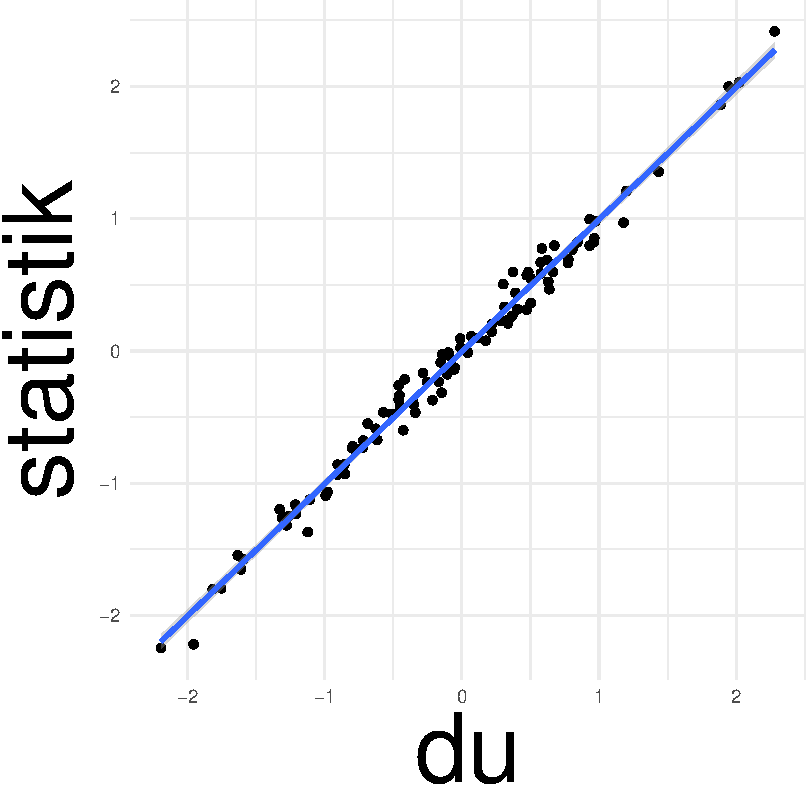
\includegraphics[width=0.33\textwidth,height=\textheight]{index_files/figure-pdf/unnamed-chunk-1-1.pdf}

}

\caption{Guter Fit}

\end{figure}%

Statistik und Du: Guter Fit!

\section{Es geht um Ihren Lernerfolg}\label{es-geht-um-ihren-lernerfolg}

Meister Yoda rät: Lesen Sie die Hinweise (Abbildung~\ref{fig-yoda}).

\begin{figure}

\centering{


\includegraphics[width=0.5\textwidth,height=\textheight]{img/yoda.jpg}

}

\caption{\label{fig-yoda}Lesen Sie die folgenden Hinweise im eigenen
Interesse}

\end{figure}%

\href{https://imgflip.com/memegenerator}{Quelle: Imgflip Memengenerator}

\subsection{Lernziele}\label{lernziele}

\begin{itemize}
\item
  Die Studentis sind mit wesentlichen Methoden der explorativen
  Datenanalyse vertraut und können diese selbständig anwenden.
\item
  Die Studentis können gängige Forschungsfragen in lineare Modelle
  übersetzen, diese auf echte Datensätze anwenden und die Ergebnisse
  interpretieren.
\end{itemize}

Kurz gesagt: Das ist ein Grundkurs in Daten zähmen.

\begin{figure}[H]

{\centering 
\includegraphics[width=0.5\textwidth,height=\textheight]{img/datenzaehmen.png}

}

\caption{Daten zähmen}

\end{figure}%

\href{https://github.com/allisonhorst/stats-illustrations}{Bildquelle:
Allison Horst, CC-BY}

\subsection{Was lerne ich hier und wozu ist das
gut?}\label{was-lerne-ich-hier-und-wozu-ist-das-gut}

\emph{Was lerne ich hier?}

Sie lernen das \emph{Handwerk der Datenanalyse} mit einem Schwerpunkt
auf Vorhersage. Anders gesagt: Sie lernen, \emph{Daten aufzubereiten}
und aus Daten \emph{Vorhersagen} abzuleiten. Zum Beispiel: Kommt ein
Student zu Ihnen und sagt ``Ich habe 42 Stunden für die Klausur gelernt,
welche Note kann ich in der Klausur erwarten?''. Darauf Ihre Antwort:
``Auf Basis meiner Daten und meines Modells müsstest du eine 2.7
schreiben!''.\footnote{Darauf dis Studenti: ``Hpmf.''}. Außerdem lernen
Sie, wie man die Güte einer Vorhersage auf Stichhaltigkeit prüft. Denn
Vorhersagen kann man ja in jeder Eckkneipe oder beim Wahrsager bekommen.
Wir wollen aber belastbare Vorhersagen und zumindest wissen, wie gut die
Vorhersagen (von jemanden) bisher waren.

\emph{Warum ist das wichtig?}

Wir wollen nicht auf Leuten vertrauen, die behaupten, sie wüssten, was
für uns richtig und gut ist. Wir wollen selber die Fakten prüfen können.

\emph{Wozu brauche ich das im Job?}

Datenanalyse spielt bereits heute in vielen Berufen eine Rolle. Tendenz
stark zunehmend.

\emph{Wozu brauche ich das im weiterem Studium?}

In Forschungsarbeiten (wie in empirischen Forschungsprojekten, etwa in
der Abschlussarbeit) ist es üblich, statistische Ergebnisse hinsichtlich
quantitativ zu analysieren.

\emph{Ist Statistik nicht sehr abstrakt?}

Der Schwerpunkt dieses Kurses liegt auf Anwenden und Tun; ähnlich dem
Erlernen eines Handwerks. Theorien und Abstraktionen stehen nur am Rand.

\emph{Gibt es auch gute Jobs, wenn man sich mit Daten auskennt?}

Das Forum (2020) berichtet zu den ``Top 20 job roles in increasing and
decreasing demand across industries'' (S. 30, Abb. 22):

\begin{enumerate}
\def\labelenumi{\arabic{enumi}.}
\tightlist
\item
  Data Analysts und Scientists
\item
  AI and Machine Learning Specialists
\item
  Big Data Specialists
\end{enumerate}

\subsection{Was ist hier das
Erfolgsgeheimnis?}\label{was-ist-hier-das-erfolgsgeheimnis}

\begin{tcolorbox}[enhanced jigsaw, colback=white, opacityback=0, arc=.35mm, titlerule=0mm, breakable, toptitle=1mm, colframe=quarto-callout-important-color-frame, title=\textcolor{quarto-callout-important-color}{\faExclamation}\hspace{0.5em}{Wichtig}, rightrule=.15mm, colbacktitle=quarto-callout-important-color!10!white, coltitle=black, leftrule=.75mm, bottomrule=.15mm, bottomtitle=1mm, opacitybacktitle=0.6, toprule=.15mm, left=2mm]

\emph{Dran bleiben} ist der Schlüssel zum Erfolg. \(\square\)

\end{tcolorbox}

\subsection{Motivieren Sie mich!}\label{motivieren-sie-mich}

Schauen Sie sich das Video mit einer
\href{https://youtu.be/jtNlzpcPr5Y}{Ansprache zur Motivation}
an.\footnote{\url{https://youtu.be/jtNlzpcPr5Y}}

\subsection{Voraussetzungen}\label{voraussetzungen}

Um von diesem Kurs am besten zu profitieren, sollten Sie Folgendes
mitbringen:

\begin{itemize}
\tightlist
\item
  Bereitschaft, Neues zu lernen
\item
  Bereitschaft, nicht gleich aufzugeben
\item
  Kenntnis grundlegender Methoden wissenschaftlichen Arbeitens
\end{itemize}

Was Sie \emph{nicht} brauchen, sind besondere Mathe-Vorkenntnisse.

\subsection{Überblick}\label{uxfcberblick}

Abb. Abbildung~\ref{fig-ueberblick} gibt einen Überblick über den
Verlauf und die Inhalte des Buches. Das Diagramm hilft Ihnen zu
verorten, wo welches Thema im Gesamtzusammenhang steht.

\begin{figure}

\centering{

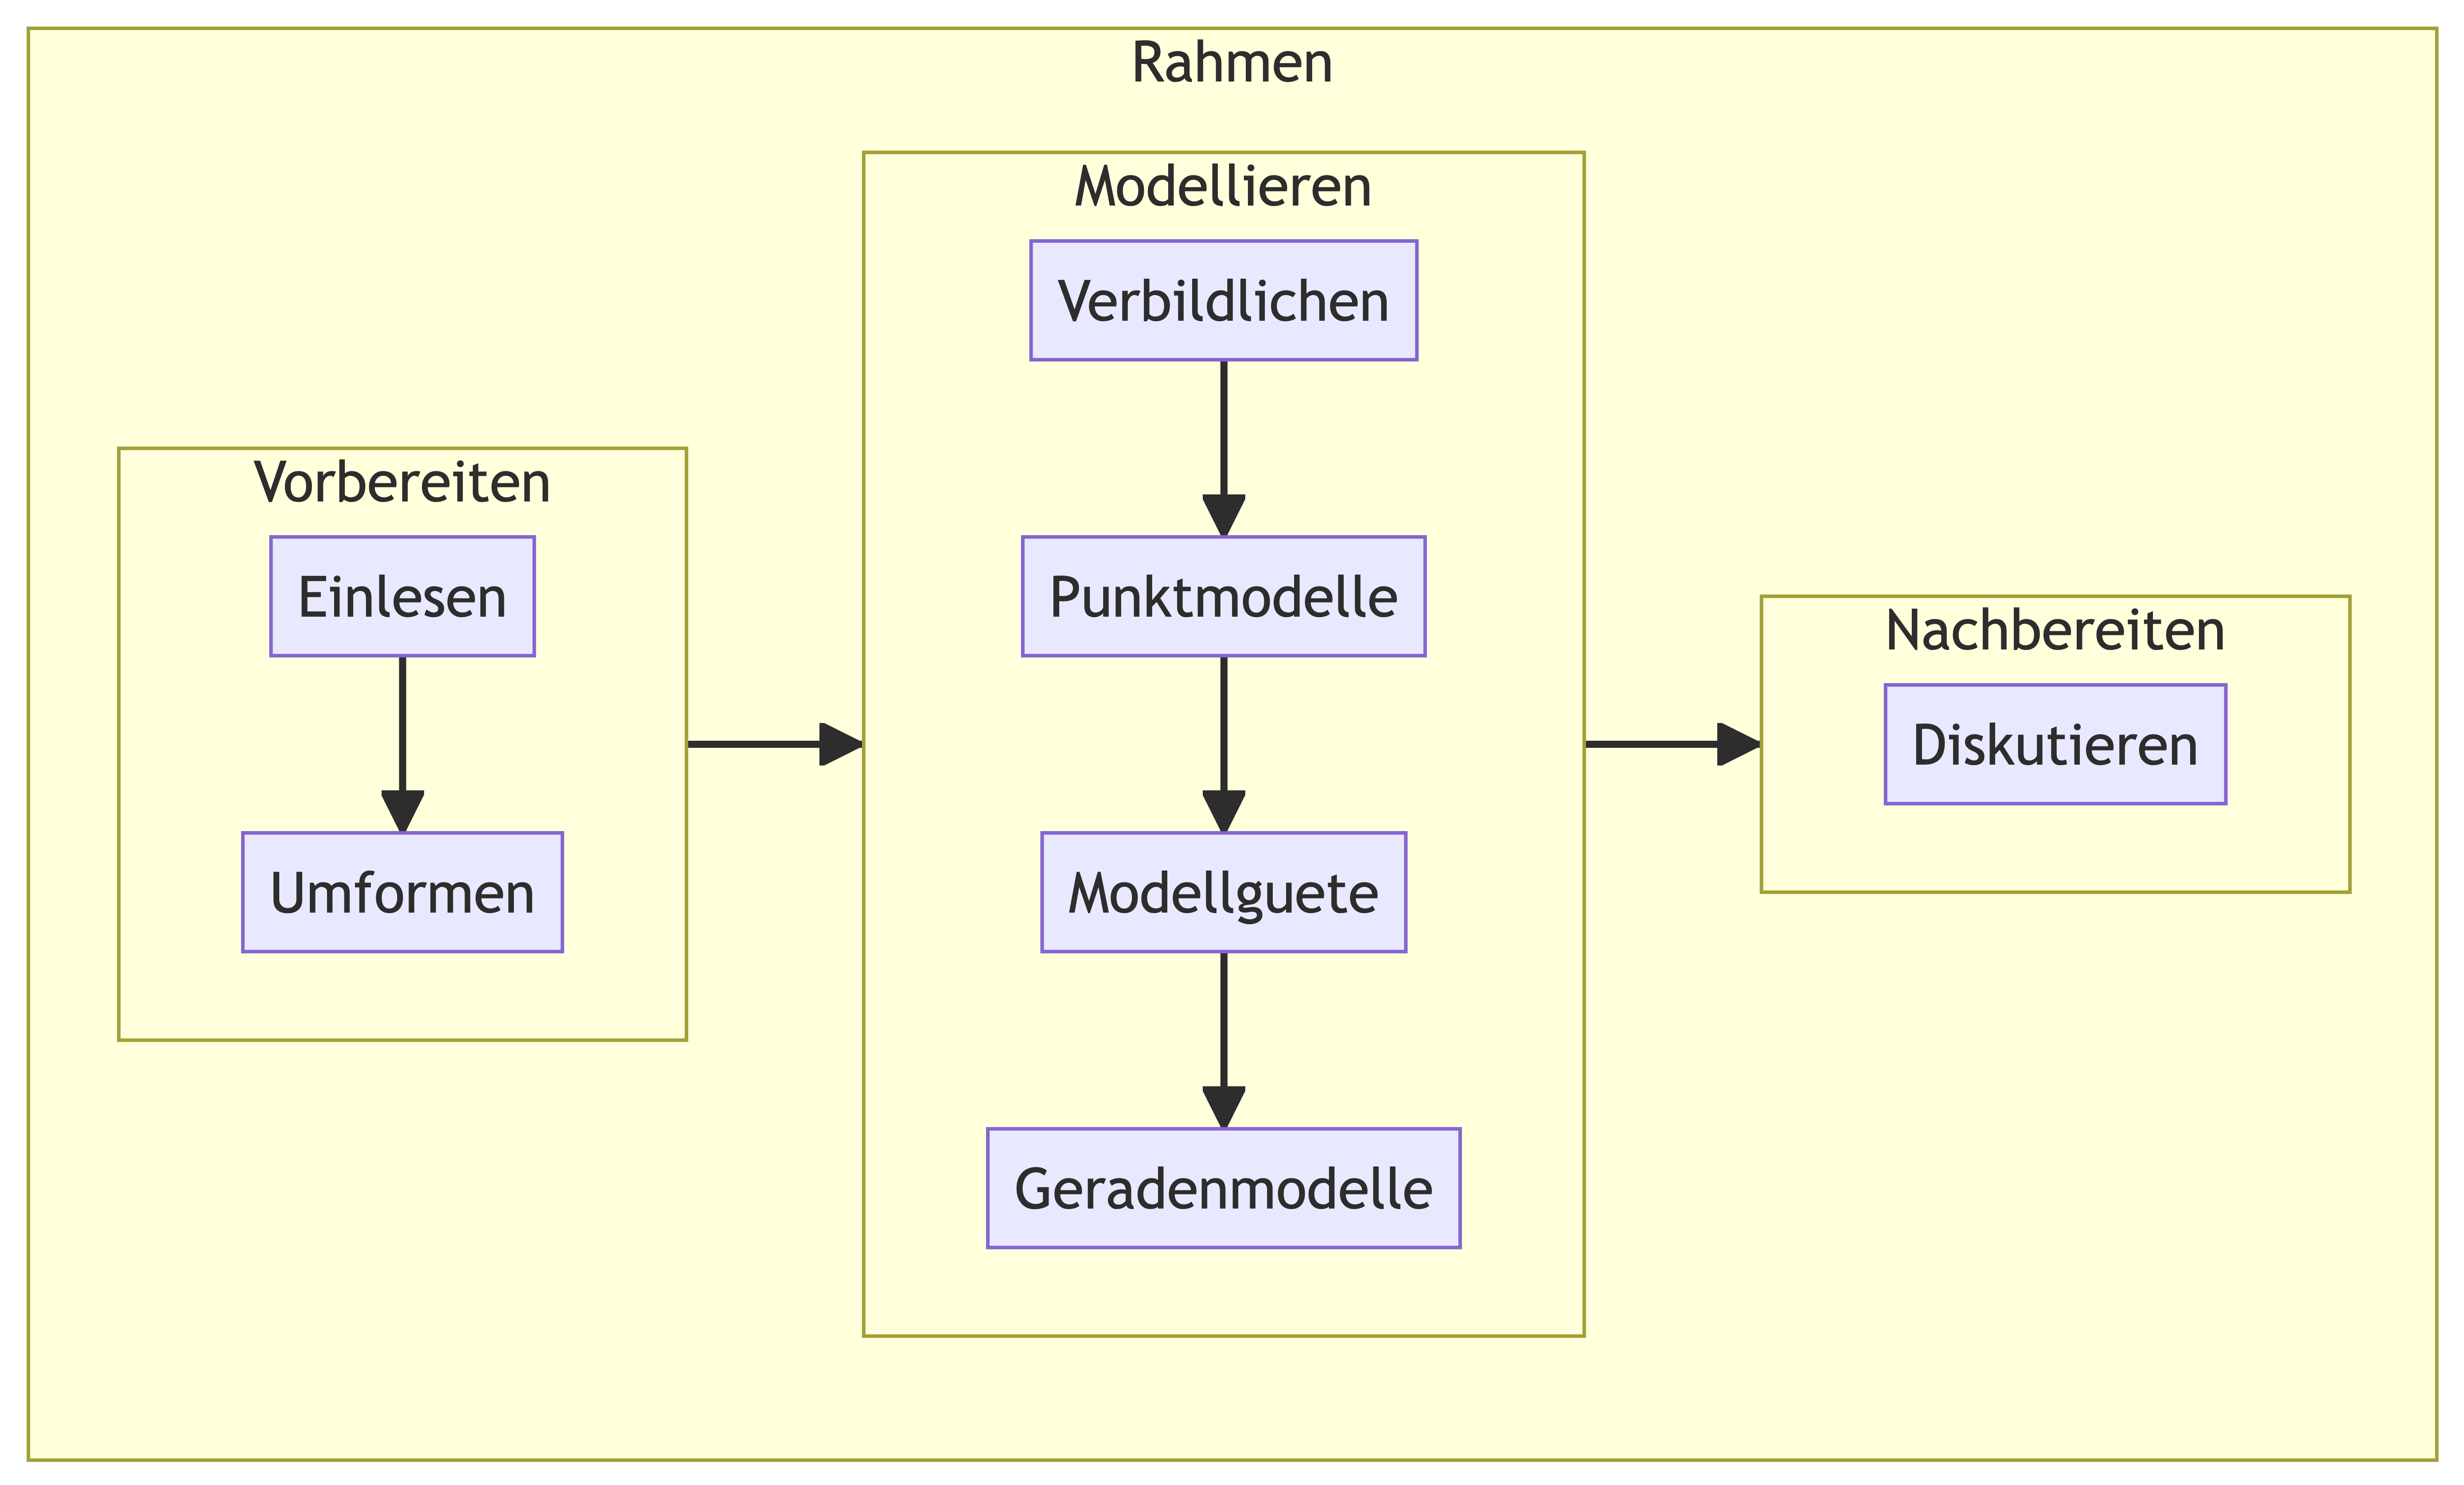
\includegraphics[width=7.24in,height=4.38in]{index_files/figure-latex/mermaid-figure-1.png}

}

\caption{\label{fig-ueberblick}Überblick über den Inhalt und Verlauf des
Buches}

\end{figure}%

Das Diagramm zeigt den Ablauf einer typischen Datenanalyse. Natürlich
kann man sich auch andere sinnvolle Darstellungen dieses Ablaufs
vorstellen.

\subsection{PDF-Version}\label{pdf-version}

Sie können die Druck-Funktion Ihres Broswers nutzen, um ein PDF-Dokument
eines Kapitels dieses Buchs zu erstellen.

\section{Software}\label{software}

Sie benötigen R, RStudio und einige R-Pakete für diesen Kurs.

\subsection{Installation}\label{installation}

\href{https://hinweisbuch.netlify.app/hinweise-software}{Hier} finden
Sie \emph{Installationshinweise.}\footnote{\url{https://hinweisbuch.netlify.app/hinweise-software}}

\subsection{Viel R (?)}\label{viel-r}

Dieses Buch enthält ``mittel'' viel R. Auf fortgeschrittene R-Techniken
wurde aber komplett verzichtet. Dem einen oder der anderen Anfänger:in
mag es dennoch ``viel Code'' erscheinen. Es wäre ja auch möglich
gewesen, auf R zu verzichten und stattdessen eine ``Klick-Software'' zu
verwenden. \href{https://jasp-stats.org/}{JASP} oder
\href{https://www.jamovi.org/}{Jamovi} sind Beispiele für tolle Software
aus dieser Kategorie. Ich glaube aber, der Verzicht auf eine
Skriptsprache (R) wäre ein schlechter Dienst an den Studentis. Mit Blick
auf eine ``High-Tech-Zukunft'' sollte man zumindest mit etwas
Computer-Code vertraut sein. Auf Computercode zu verzichten erschiene
mir daher fahrlässig für die ``Zukunftsfestigkeit'' der Ausbildung.

\section{Hinweise}\label{hinweise}

\begin{itemize}
\item
  📺
  \href{https://www.youtube.com/channel/UCkvdtj8maE7g-SOCh4aDB9g}{YouTube-Playlists
  zu Statistik}
\item
  \href{https://hinweisbuch.netlify.app/hinweise-lernhilfen-frame}{Lernhilfen}
\item
  \href{https://hinweisbuch.netlify.app/hinweise-didaktik-frame}{Didaktik}
\item
  \href{https://hinweisbuch.netlify.app/hinweise-unterricht-frame}{Unterrichtsorganisation}
\item
  Der Unterricht zu diesem Modul wird nur ein Mal pro Jahr angeboten
  (also nur jedes zweite Semester).
\item
  Eine Prüfung in diesem Modul ist jedes Semester möglich.
\end{itemize}

\section{Prüfung}\label{pruxfcfung}

\href{https://hinweisbuch.netlify.app/hinweise-pruefung-prognosewettbewerb-frame}{Im
Hinweisbuch} finden Sie Hinweise zur Prüfung.\footnote{\url{https://hinweisbuch.netlify.app/hinweise-pruefung-prognosewettbewerb-frame}}

\section{Zum Autor}\label{zum-autor}

Nähere Hinweise zum Autor dieses Buch, Sebastian Sauer, finden Sie
\href{https://sebastiansauer-academic.netlify.app/}{hier}.\footnote{\url{https://sebastiansauer-academic.netlify.app/}}
Dort gibt es auch einen Überblick über
\href{https://sebastiansauer-academic.netlify.app/\#ebooks}{weitere
Bücher des Autors zum Themenkreis Datenanalyse}.\footnote{\textless(https://sebastiansauer-academic.netlify.app/\#ebooks\textgreater{}}

\section{Nomenklatur}\label{nomenklatur}

\subsection{Griechische Buchstaben}\label{sec-greek}

In diesem Buch werden ein paar (wenige) griechische Buchstaben
verwendet, die in der Statistik üblich sind.

Häufig werden \emph{griechische} Buchstaben verwendet, um eine
Grundgesamtheit (Population) zu beschreiben (die meistens unbekannt
ist). Lateinische (``normale'') Buchstaben werden demgegenüber
verwendet, um eine Stichprobe (Datensatz, vorliegende Daten) zu
beschreiben.

Tabelle~\ref{tbl-griech} stellt diese Buchstaben zusammen mit ihrer
Aussprache und Bedeutung vor.

\begin{longtable}[]{@{}lllr@{}}
\caption{Griechische Buchstaben, die in diesem Buch verwendet
werden.}\label{tbl-griech}\tabularnewline
\toprule\noalign{}
Zeichen & Aussprache & Buchstabe & Bedeutung in der Statistik \\
\midrule\noalign{}
\endfirsthead
\toprule\noalign{}
Zeichen & Aussprache & Buchstabe & Bedeutung in der Statistik \\
\midrule\noalign{}
\endhead
\bottomrule\noalign{}
\endlastfoot
\(\beta\) & beta & b & Regressionskoeffizent \\
\(\mu\) & mü & m & Mittelwert \\
\(\sigma\) & sigma & s & Streuung \\
\(\Sigma\) & Sigma & S & Summenzeichen \\
\(\rho\) & rho & r & Korrelation (nach Pearson) \\
\end{longtable}

Mehr griechische Buchstaben finden sich
\href{https://de.wikipedia.org/wiki/Griechisches_Alphabet}{z.B. in
Wikipedia}.

\section{Zitation}\label{zitation}

Bitte zitieren Sie dieses Buch wie folgt:

\begin{quote}
Sauer, S. (2024). \emph{Statistik1}. https://statistik1.netlify.app/
\end{quote}

Hier sind die maschinenlesbaren Zitationsinfos (Bibtex-Format), die Sie
in Ihre Literatursoftware importieren können:

\begin{verbatim}
@book{sauer_statistik1,
    title = {Statistik1},
    rights = {CC-BY-NC},
    url = {https://statistik1.netlify.app/},
    author = {Sauer, Sebastian},
    date = {2024},
}
\end{verbatim}

Hier ist die DOI:

\href{https://zenodo.org/doi/10.5281/zenodo.10082517}{10.5281/zenodo.10082517}

\section{Reproduzierbarkeit}\label{reproduzierbarkeit}

Die verwendeten R-Pakete sind mit
\href{https://rstudio.github.io/renv/index.html}{renv}
dokumentiert.\footnote{\url{https://rstudio.github.io/renv/index.html}}

Der Quellcode ist \href{https://github.com/sebastiansauer/statistik1}{in
diesem Github-Repo} dokumentiert.\footnote{\url{https://github.com/sebastiansauer/statistik1}}

Dieses Dokument wurde erzeugt am/um 2024-04-07 17:58:12.

\section{Literatur}\label{literatur}

\part{Organisatorisches}

\part{Vorbereiten}

\chapter{Rahmen}\label{rahmen}

\[
\definecolor{ycol}{RGB}{230,159,0}
\definecolor{modelcol}{RGB}{86,180,233}
\definecolor{errorcol}{RGB}{0,158,115}
\definecolor{beta0col}{RGB}{213,94,0}
\definecolor{beta1col}{RGB}{0,114,178}
\definecolor{xcol}{RGB}{204,121,167}
\]

\section{Lernsteuerung}\label{lernsteuerung}

\subsection{Standort im Lernpfad}\label{standort-im-lernpfad}

Abbildung~\ref{fig-ueberblick} zeigt den Standort dieses Kapitels im
Lernpfad und gibt damit einen Überblick über das Thema dieses Kapitels
im Kontext aller Kapitel.

Abbildung~\ref{fig-tidy5} zeigt, dass unser Vorgehen in diesem Buch
einem Fließband gleicht: Schritt für Schritt, in der richtigen
Reihenfolge, vom Anfang bis Ende, erarbeiten wir unser
``Datenprodukt''.\footnote{Quelle: Allison Horst, CC-by,
  \url{https://github.com/allisonhorst/stats-illustrations}}

\begin{figure}

\centering{

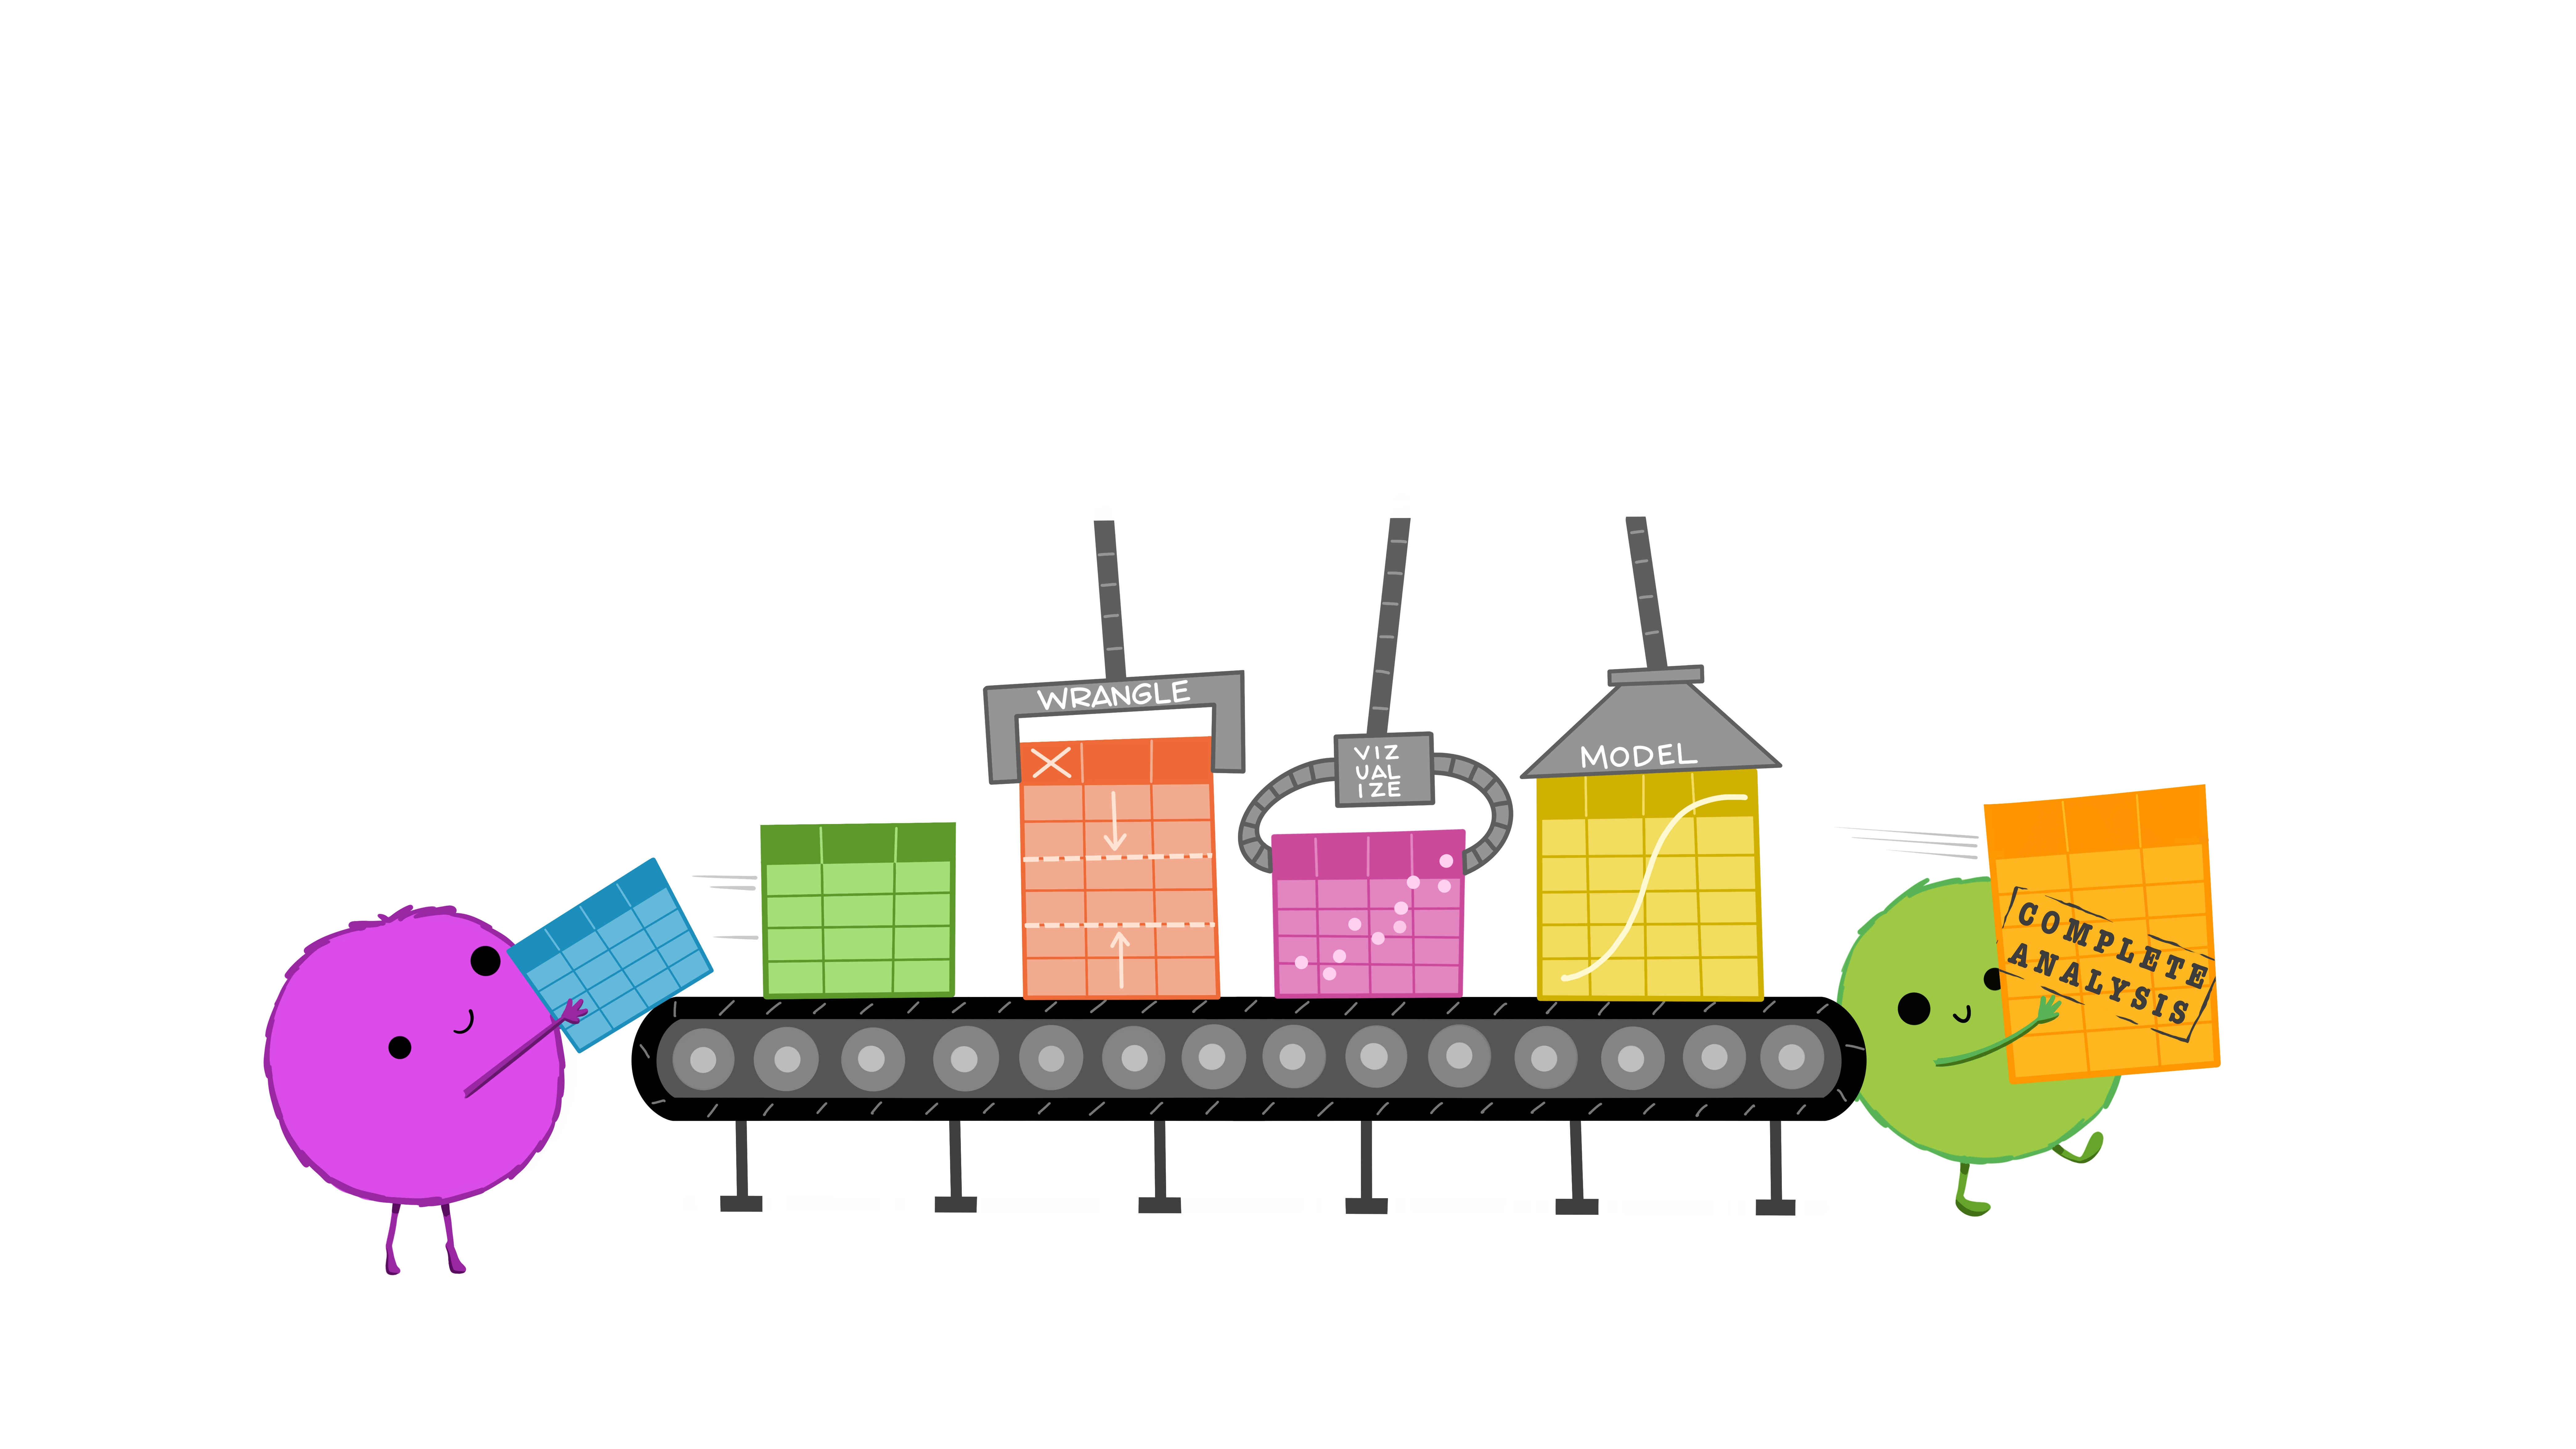
\includegraphics[width=0.75\textwidth,height=\textheight]{img/tidydata_5.jpg}

}

\caption{\label{fig-tidy5}Datenanalyse als eine Abfolge am Fließband}

\end{figure}%

\subsection{Lernziele}\label{lernziele-1}

\begin{itemize}
\tightlist
\item
  Sie können eine Definition von Statistik wiedergeben.
\item
  Sie können eine Definition von Daten wiedergeben.
\item
  Sie können den Begriff Tidy-Daten erläutern.
\item
  Sie können Beispiele für verschiedene Skalenniveaus nennen.
\end{itemize}

\subsection{Einstieg}\label{einstieg}

\begin{exercise}[Hallo,
Statistik]\protect\hypertarget{exr-einstieg}{}\label{exr-einstieg}

Gehen Sie in eine kleine Gruppe zusammen (3-4 Personen). Stellen Sie
sich anhand der Schlagworte einander vor:

\begin{enumerate}
\def\labelenumi{\arabic{enumi}.}
\tightlist
\item
  Name
\item
  (wissenschaftliche) Interessen
\item
  Erwartung an diesen Kurs \(\square\)
\end{enumerate}

\end{exercise}

\begin{exercise}[Frag
jetzt]\protect\hypertarget{exr-fragjetzt}{}\label{exr-fragjetzt}

Die Lehrkraft stellt Ihnen ein Forum zur Verfügung, auf dem Sie
\emph{anonym} Fragen an die Lehrkraft richten können (z.B. auf
\href{https://frag.jetzt/home}{frag.jetzt}).

Stellen Sie dort Ihre Fragen ein; voten Sie die Fragen Ihrer
Kommilitonis auf oder ab. Die Lehrkraft beantwortet dann die Fragen mit
den meisten Upvotes. \(\square\)

\end{exercise}

\subsection{Erfolsgrezept}\label{erfolsgrezept}

Ihren Lernerfolg kann man als von drei Faktoren abhängig betrachten: 1)
Ihrer Lehrkraft, 2) Ihrer Mitarbeit im Unterricht und 3) Ihrem
Eigenstudium zuhause (Vor- bzw. Nachbereitung des Unterrichts), s.
Abbildung~\ref{fig-erfolgsrezept}.

\begin{figure}

\centering{

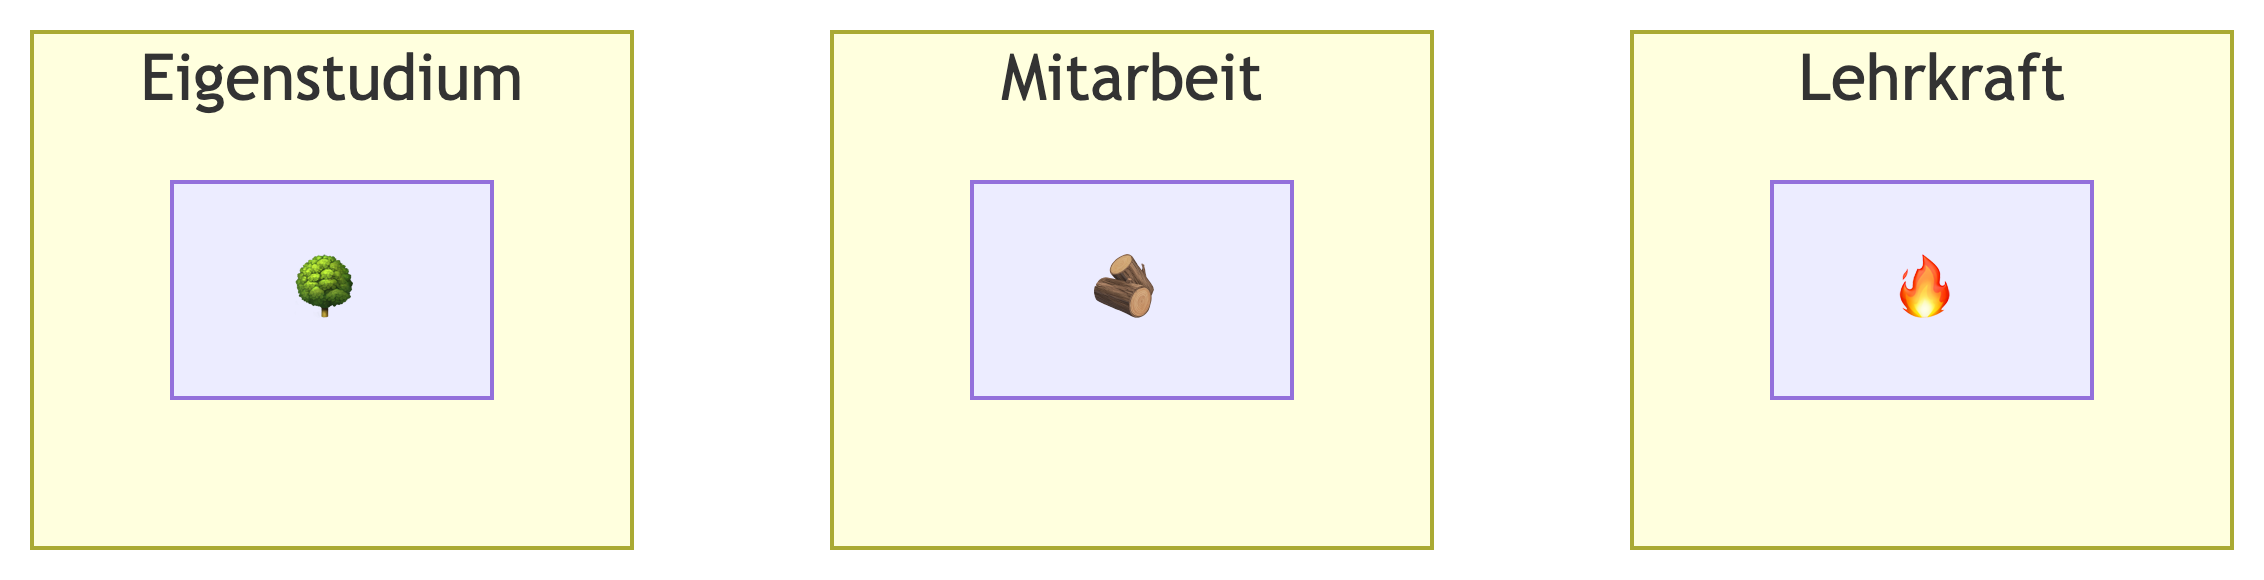
\includegraphics[width=5.35in,height=1.06in]{010-rahmen_files/figure-latex/mermaid-figure-1.png}

}

\caption{\label{fig-erfolgsrezept}Ihr Lernerfolg besteht aus drei
Komponenten: Der Lehrkraft, Ihrer Konzentration im Unterricht und Ihrer
Vor- bzw. Nachbereitung zuhause.}

\end{figure}%

Eine gute Lehrkraft ist wie der Funke, der eine (Lern-)Flamme entzündet.
Aber es braucht Brennmaterial, einen Holzscheit, das ist Ihre
Konzentration im Unterricht. Ein Holzscheit alleine ist aber nicht
nachhaltig, es braucht viel mehr Brennmaterial, um das Feuer am Leben zu
halten: Ihr Eigenstudium, das stetige, selbständige Beschäftigen mit der
Materie.

\section{Was ist Statistik und wozu ist sie
gut?}\label{was-ist-statistik-und-wozu-ist-sie-gut}

\begin{exercise}[Nutzen von
Statistik]\protect\hypertarget{exr-nutzen-statistik}{}\label{exr-nutzen-statistik}

🏋️‍♀️ Fragen Sie ChatGPT, was der Nutzen von Statistik ist. Diskutieren Sie
die Antwort. \(\square\)

\end{exercise}

\begin{tcolorbox}[enhanced jigsaw, colback=white, opacityback=0, arc=.35mm, titlerule=0mm, breakable, toptitle=1mm, colframe=quarto-callout-note-color-frame, title=\textcolor{quarto-callout-note-color}{\faInfo}\hspace{0.5em}{Hinweis}, rightrule=.15mm, colbacktitle=quarto-callout-note-color!10!white, coltitle=black, leftrule=.75mm, bottomrule=.15mm, bottomtitle=1mm, opacitybacktitle=0.6, toprule=.15mm, left=2mm]

In diesem Buch werden die Begriffe \emph{Statistik}, \emph{Datenanalyse}
und \emph{Data Science} synonym verwendet.\(\square\)

\end{tcolorbox}

Hm. Vielleicht fragen wir mal ChatGPT, was es unter Statistik versteht:

\begin{quote}
👨 Was ist Statistik? Bitte definiere verständlich.
\end{quote}

\begin{quote}
🤖 Statistik ist eine Wissenschaft, die sich mit der Sammlung, Analyse,
Interpretation, Präsentation und Übertragung von Daten beschäftigt. Ziel
ist es, Muster und Trends in den Daten zu erkennen und verlässliche
Schlussfolgerungen über eine größere Gruppe (z.B. Bevölkerung) auf der
Basis einer Stichprobe (Teilmenge) zu treffen. Die Statistik hilft uns
bei der Beantwortung von Fragen, indem sie uns dabei hilft, die
Unsicherheit in den Daten zu messen und zu verstehen\footnote{Release
  2023-Jan}.
\end{quote}

Es gibt mehrere Definition von Statistik; hier ist eine.

\begin{definition}[Statistik]\protect\hypertarget{def-statistik}{}\label{def-statistik}

Statistik fasst Daten zusammen, um wesentliche Informationen den Daten
zu entnehmen und beschreibt die Ungewissheit unserer Schlüsse (Poldrack,
2023); Kaplan (2009) .\(\square\)

\end{definition}

Betrachten wir die zwei Bestimmungsstücke einer Definition von Statistik
genauer:

\begin{enumerate}
\def\labelenumi{\arabic{enumi}.}
\tightlist
\item
  Daten zusammenfassen
\item
  Ungewissheit beschreiben
\end{enumerate}

\subsection{Daten zusammenfassen}\label{daten-zusammenfassen}

Abbildung~\ref{fig-zsmnfassen} verdeutlicht das Prinzip des
Zusammenfassens von Daten. Anschaulich gesprochen: Eine Menge von Zahlen
wird zu einer einzelnen Zahl ``zusammengedampt''. Eine einzelne Zahl ist
wesentlich besser zu verstehen als eine große Menge von Zahlen. Bei
vielen Zahlen würde man den Überblick verlieren.

\begin{figure}

\begin{minipage}{0.50\linewidth}

\centering{

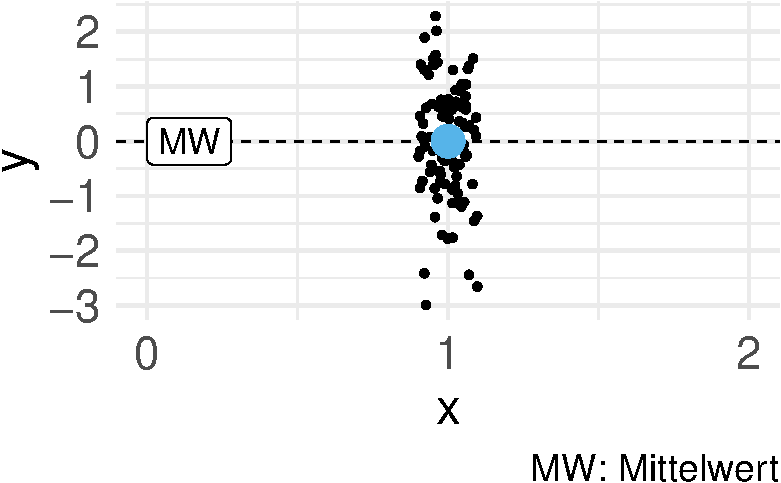
\includegraphics{010-rahmen_files/figure-pdf/fig-zsmnfassen-1.pdf}

}

\subcaption{\label{fig-zsmnfassen-1}Zusammenfassen einer Variable zu
einem Punktwert, hier zum Mittelwert}

\end{minipage}%
%
\begin{minipage}{0.50\linewidth}

\centering{

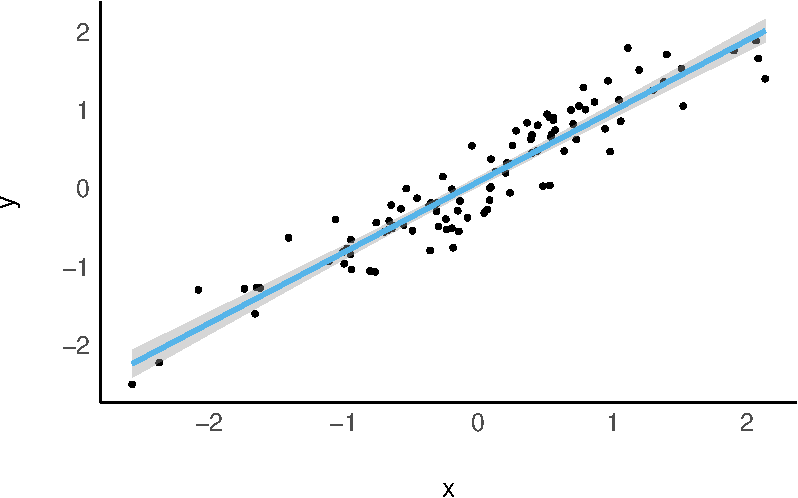
\includegraphics{010-rahmen_files/figure-pdf/fig-zsmnfassen-2.pdf}

}

\subcaption{\label{fig-zsmnfassen-2}Zusammenfassen zweier Variablen zu
einer Geraden}

\end{minipage}%

\caption{\label{fig-zsmnfassen}Daten zusammenfassen}

\end{figure}%

\subsection{Unterschiedlichkeit
messen}\label{unterschiedlichkeit-messen}

Eine allgegenwärtige Tatsache ist, dass die Dinge der Welt sich
unterscheiden, etwa, dass Exemplare einer Gattung sich unterscheiden. So
sind nicht alle Menschen gleich groß, nicht alle Bücher gleich lang oder
nicht alle Tage gleich warm.

Ein zentrales Vorgehen bei statistischen Analysen ist es, die
\emph{Unterschiedlichkeit der Dinge} zu beschreiben, präziser gesagt:
die \emph{Variation zu quantifizieren}. Betrachten wir dazu das Beispiel
in s. Abbildung~\ref{fig-groesse}.

\begin{figure}

\centering{

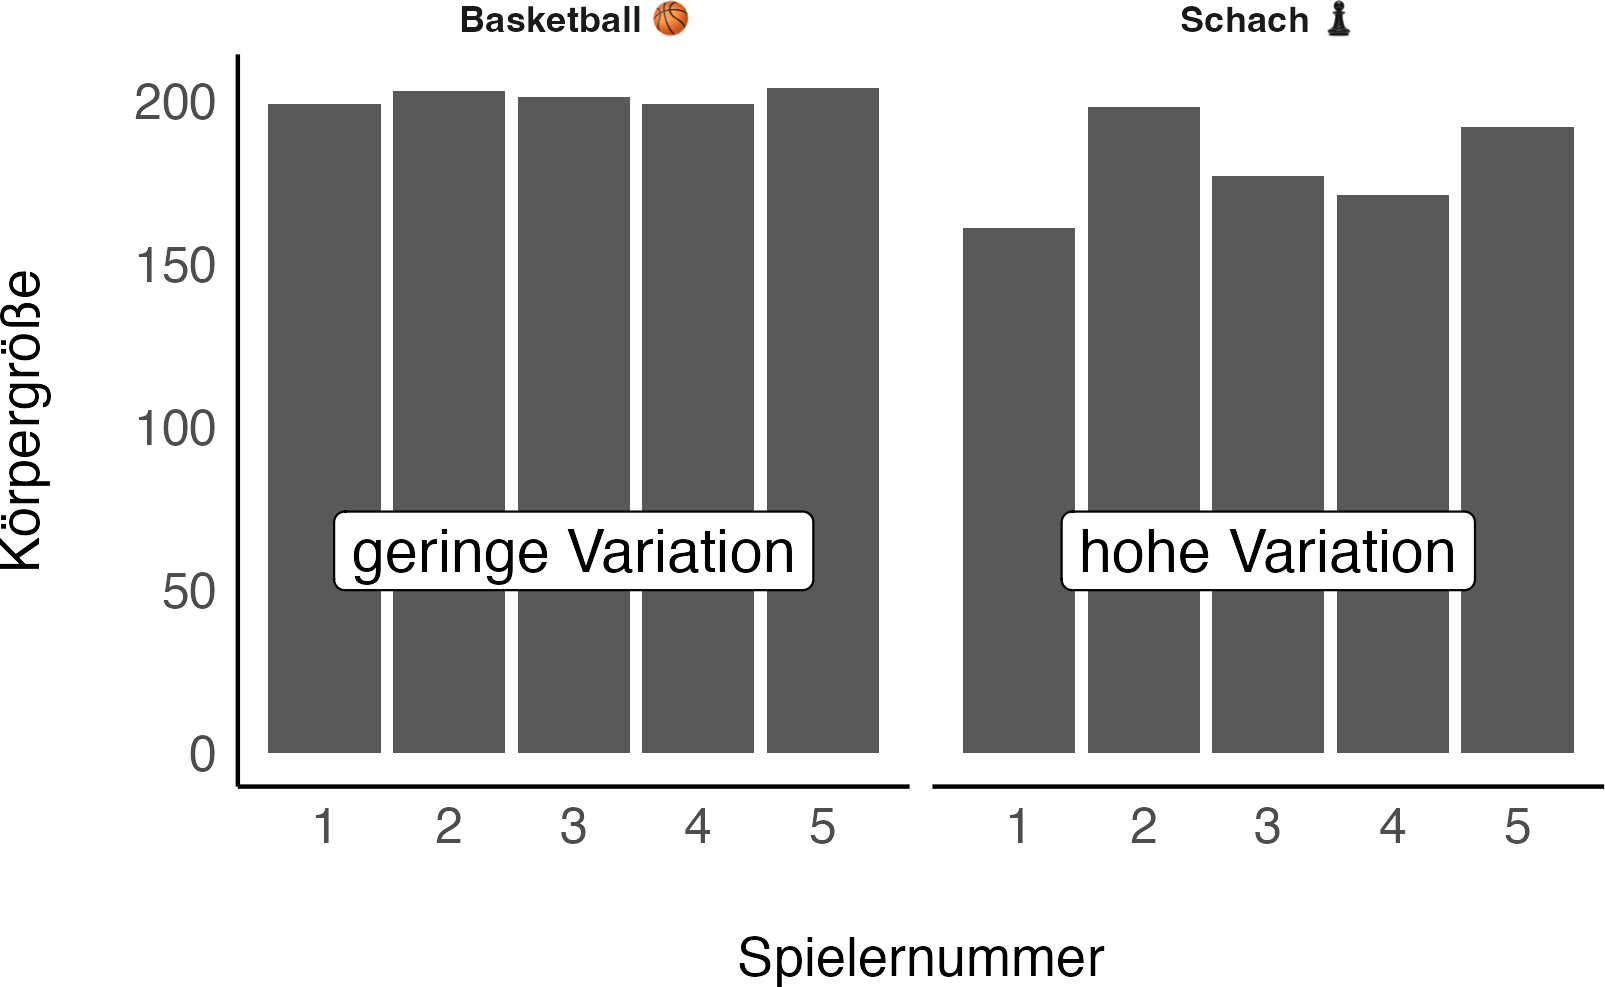
\includegraphics{010-rahmen_files/figure-pdf/fig-groesse-1.png}

}

\caption{\label{fig-groesse}Wenig Variation in der Körpergröße bei den
Basketballern. Alles lange Kerle. Viel Variation bei den Schachspielern:
Manche sind klein, ander groß.}

\end{figure}%

Bei den Basketballern gibt es \emph{geringe} Variation in der
Körpergröße - alle sind groß, ähnlich groß. Bei den Schachspielern gibt
es (im Verhältnis) \emph{hohe} Variation: Einige Personen sind groß,
andere klein.

Die Variation (auch ``Variabilität'' genannt) kann man auch gut so
darstellen wie in s. Abbildung~\ref{fig-variab} gezeigt.

\begin{figure}

\centering{

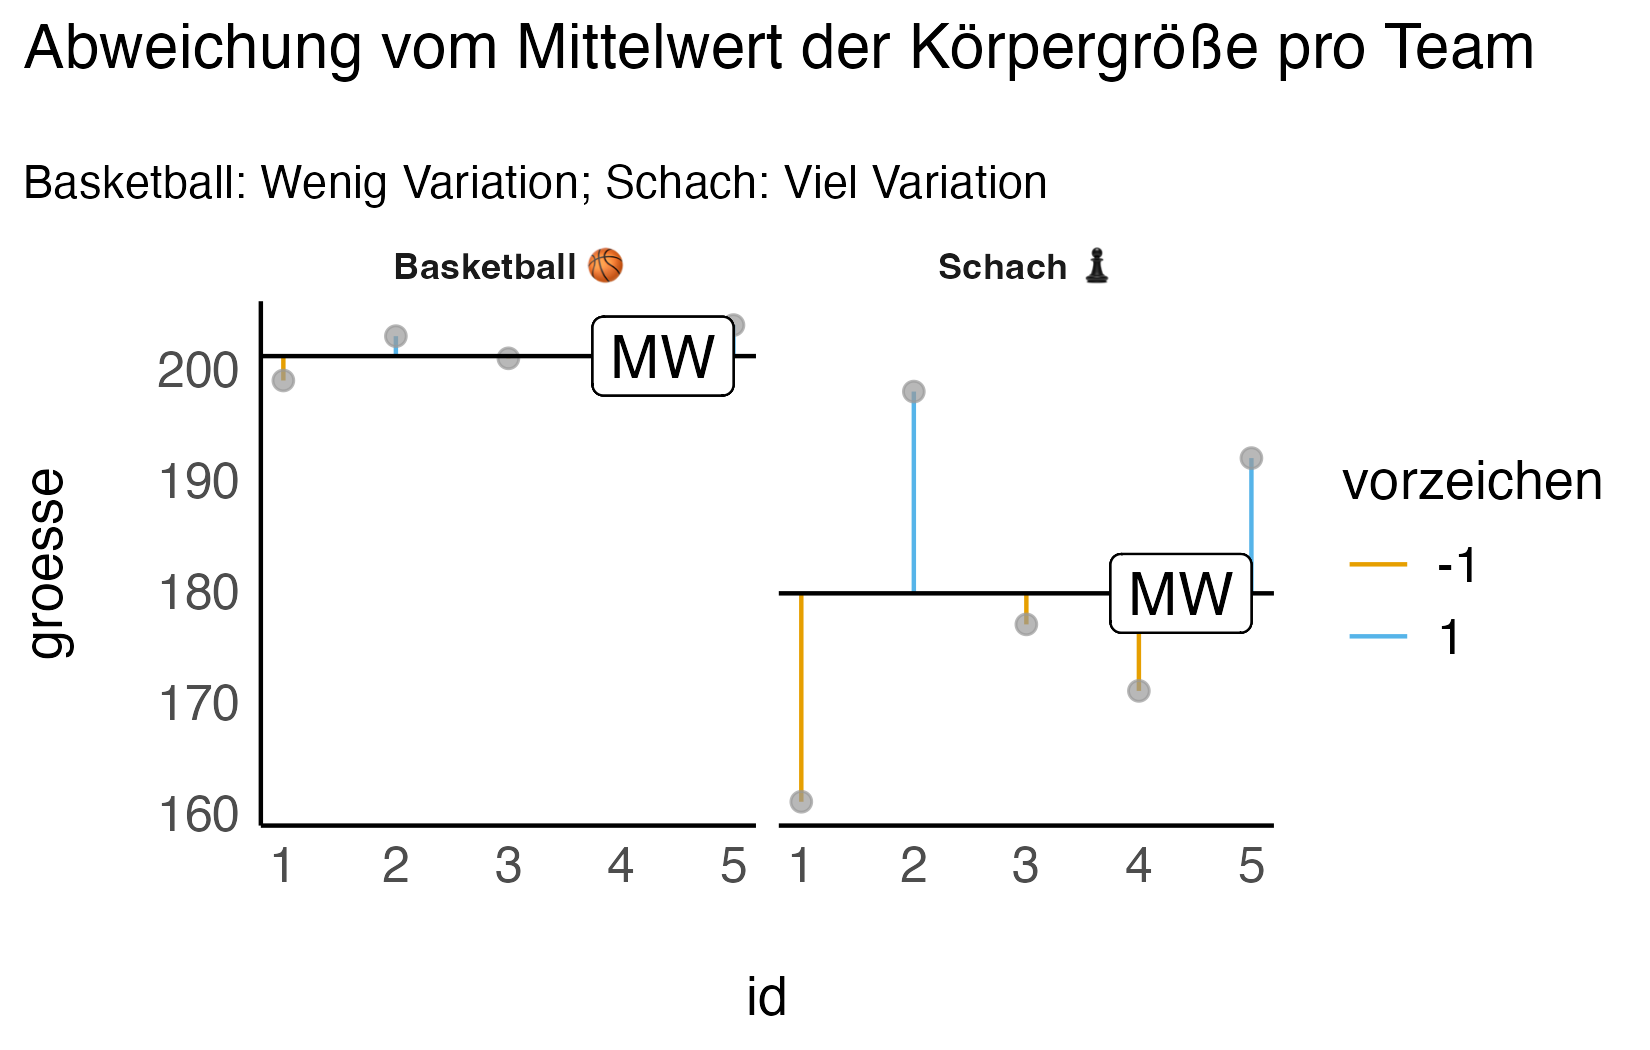
\includegraphics{010-rahmen_files/figure-pdf/fig-variab-1.png}

}

\caption{\label{fig-variab}Die Abweichungen der einzelnen Personen von
der mittleren Körpergröße ihres Teams}

\end{figure}%

Eine \emph{Abweichung} (auch \emph{Residuum}) genannt, zeigt hier die
Differenz von Mittelwert und dem Wert der Körpergröße bei der jeweiligen
Person. Wenn wir allgemein von einer Person \(i\) sprechen, Das Merkmal
\emph{Körpergröße} mit \(X\) bezeichnen und den Mittelwert der
Körpergröße als \(\bar{x}\) (``x quer''), dann können wir knapp und
präzise das Residuum der \(i\)-ten Person mit \(r_i\) bezeichnen und
entsprechend definieren.

\begin{definition}[Residuum]\protect\hypertarget{def-residuum}{}\label{def-residuum}

Das Residuum des Merkmals \(X\) der \(i\)-ten Beobachtung ist definiert
als die Differenz vom Wert \(x_i\) und einem Referenzwert, etwa dem
Mittelwert, \(\bar{x}\):

\(r_i = x_i - \bar{x}\). \(\square\)

\end{definition}

\section{Was ist das Ziel Ihrer
Analyse?}\label{was-ist-das-ziel-ihrer-analyse}

\subsection{Arten von Zielen}\label{arten-von-zielen}

\begin{figure}

\centering{

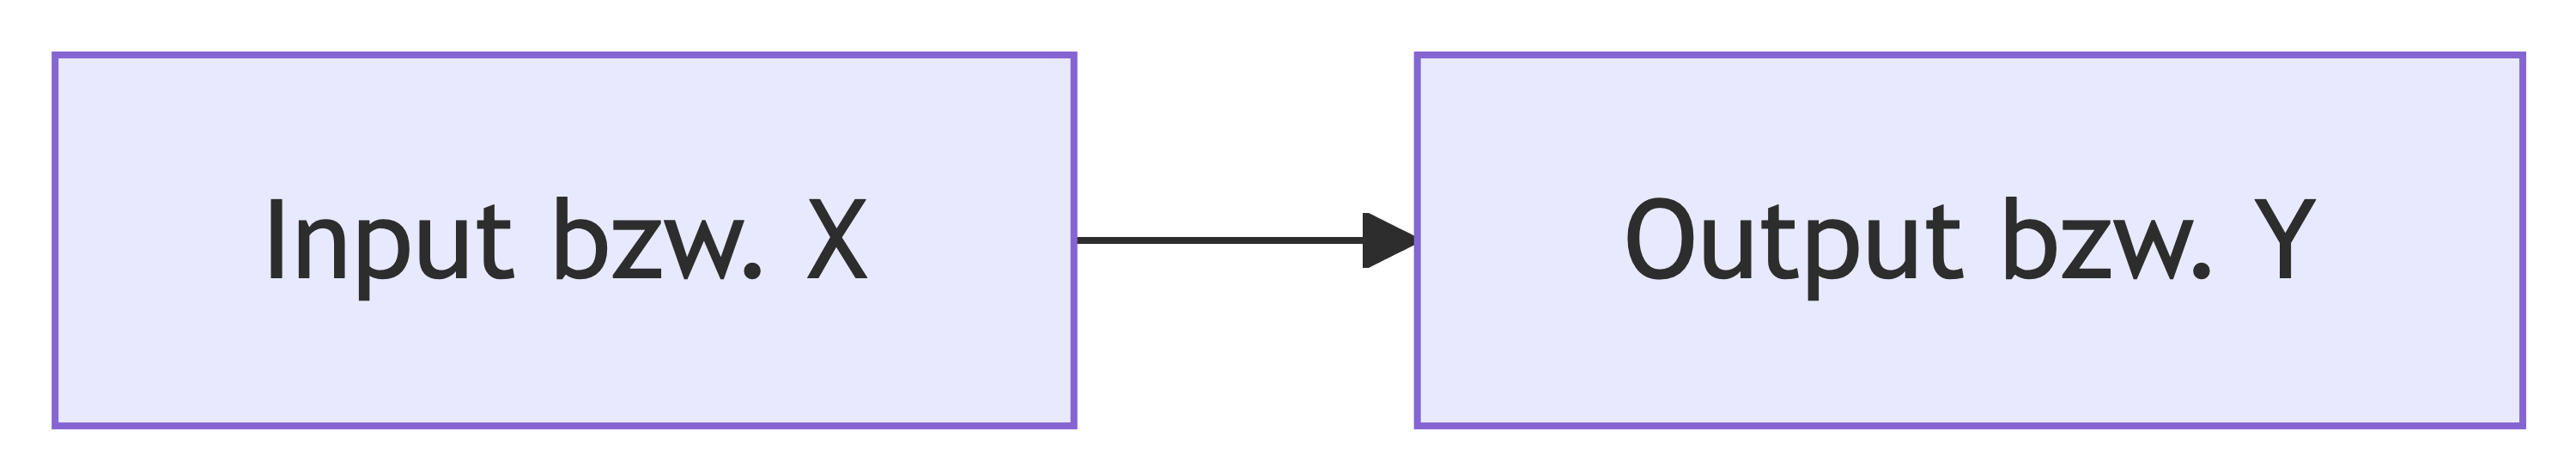
\includegraphics[width=4.84in,height=1.04in]{010-rahmen_files/figure-latex/mermaid-figure-6.png}

}

\caption{\label{fig-ziele}Zielarten einer Datenanalyse}

\end{figure}%

Beispiele für die einzelnen Zielarten der Datenanalyse:

\begin{itemize}
\tightlist
\item
  \emph{Beschreiben}: ``Wie groß ist der Gender-Paygap in der Branche X
  im Zeitraum Y?''
\item
  \emph{Vorhersagen}: Wenn ich 100 Stunden auf die Statistikklausur
  lernen, welche Note kann ich dann erwarten?
\item
  \emph{Erklären}: Wie viel bringt mir das Lernen auf die
  Statistikklausur?
\end{itemize}

\begin{exercise}[]\protect\hypertarget{exr-ziele-stat}{}\label{exr-ziele-stat}

Benennen Sie Beispiele für die die drei Zielarten von Datenanalysen!
\(\square\)

\end{exercise}

\subsection{Forschungsfrage}\label{forschungsfrage}

Eine Forschungsfrage ist die Leitfrage Ihrer Analyse. Sie definiert, was
Sie herausfinden wollen. Häufig sind Forschungsfragen so aufgebaut:

\begin{quote}
Hat X einen Einfluss auf Y?
\end{quote}

Eine Forschungsfrage weist häufig folgende Struktur auf, s.
Abbildung~\ref{fig-fo-struktur}.

\begin{figure}

\centering{

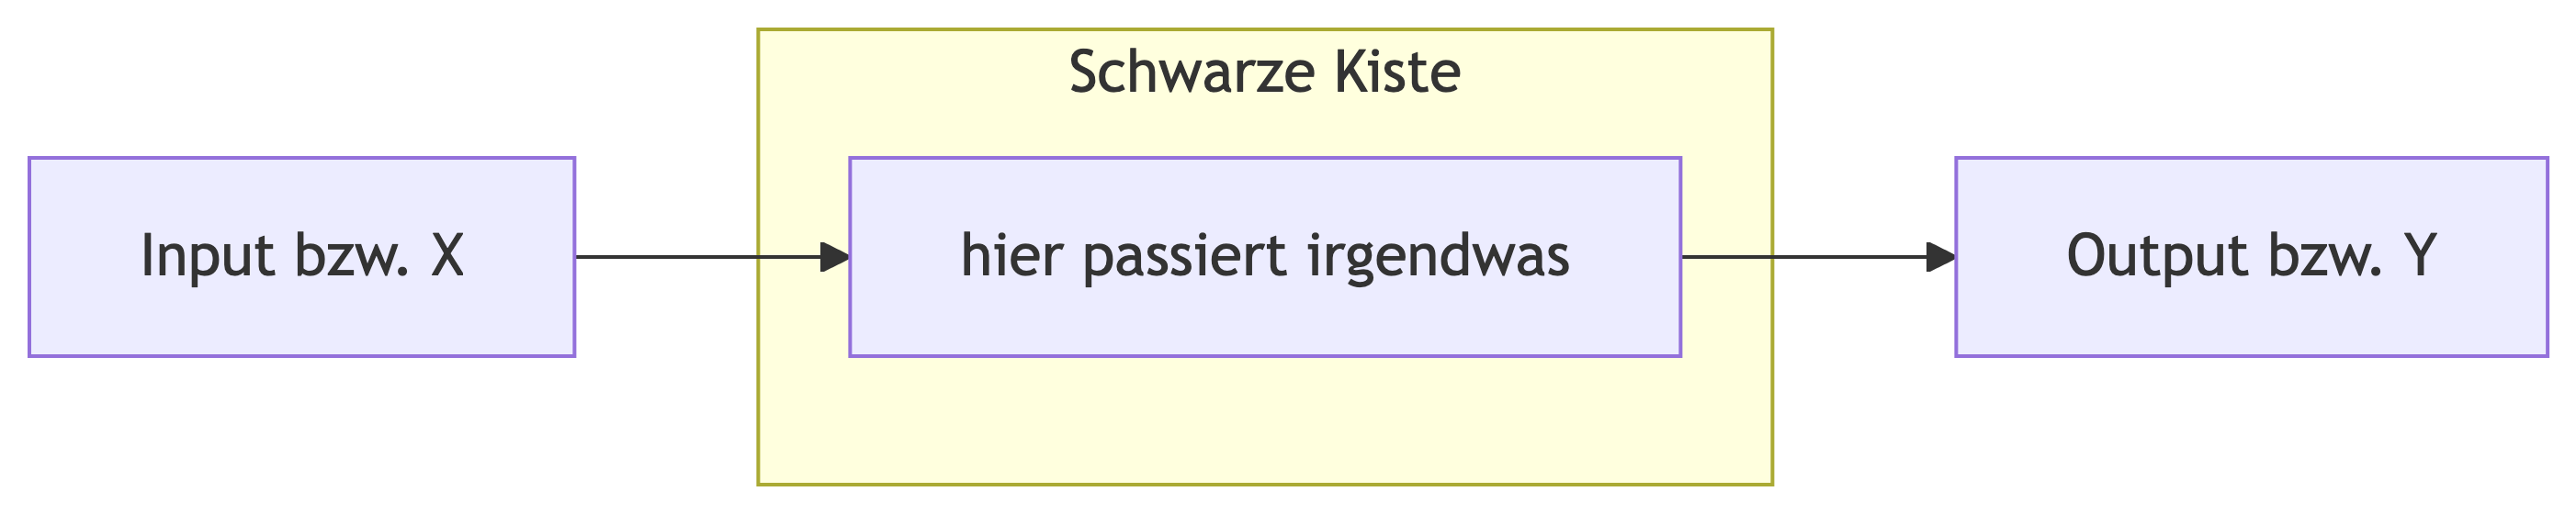
\includegraphics[width=5.9in,height=1.24in]{010-rahmen_files/figure-latex/mermaid-figure-5.png}

}

\caption{\label{fig-fo-struktur}Struktur eine Forschungsfrage}

\end{figure}%

\begin{example}[Forschungsfrage
1]\protect\hypertarget{exm-fofrage1}{}\label{exm-fofrage1}

~

\begin{quote}
Hat Lernen (X) einen Einfluss auf den Prüfungserfolg (Y)? Verringert
Joggen (X) die Menge des Hüftgolds (Y)? Um welchen Betrag erhöht sich
der Umsatz (Y), wenn wir 1000€ mehr Werbung ausgeben? (X)\(\square\)
\end{quote}

\end{example}

\begin{example}[Forschungsfrage
2]\protect\hypertarget{exm-fofrage2}{}\label{exm-fofrage2}

Nach dem Studium haben Sie bei einem großen Online-Auktionshaus
angeheuert. Da Sie angaben, sich im Studium \st{intensiv} etwas mit
Statistik beschäftigt zu haben, hat man Sie in die
F\&E-Abteilung\footnote{Forschung und Entwicklung} gesteckt. Heute ist
es Ihre Aufgabe, Auktionen zur Spielekonsole
\href{https://www.nintendo.de/Wii/Wii-94559.html}{Wii} zu untersuchen,
genauer gesagt, geht es um das Spiel
\href{https://www.nintendo.de/Spiele/Wii/Mario-Kart-Wii-281848.html\#_bersicht}{Mariokart}.
Ihre Forschungsfrage lautet:

\begin{quote}
Welche Produktmerkmale stehen mit einem hohen Verkaufserlös in
Zusammenhang?\(\square\)
\end{quote}

\end{example}

\begin{example}[Handynutzung und
Konzentrationsfähigkeit]\protect\hypertarget{exm-braindrain}{}\label{exm-braindrain}

Eine Forschungsfrage könnte lauten zum Thema Handynutzung:

\begin{quote}
Verringert intensive Handynutzung die Konzentrationsfähigkeit?
\(\square\)
\end{quote}

\end{example}

\begin{example}[Aus der Forschung: Smartphone-Brain-Drain
📱🧠🚫]\protect\hypertarget{exm-braindrain2}{}\label{exm-braindrain2}

Ward et al. (2017) untersuchten die Forschungsfrage, ob die bloße
Gegenwart eines Handies (z.B. wenn es vor Ihnen auf dem Tisch liegt)
dazu führt, dass man abgelenkt wird und daher schlechtere kognitive
Leistungen zeigt.

Leider schreiben die Autoren Ihre Hypothese nicht glasklar, aber
implizit ist obige Hypothese herauszulesen:

\begin{quote}
First, smartphones may redirect the orientation of conscious attention
away from the focal task and toward thoughts or behaviors associated
with one's phone. Prior research provides ample evidence that \ldots{}
this digital distraction adversely affects both performance \ldots{} and
enjoyment.
\end{quote}

Später formulieren Sie Ihre Hypothese noch genauer:

\begin{quote}
In two experiments, we test the hypothesis that the mere presence of
one's own smartphone reduces available cognitive capacity.
\end{quote}

Die Ergebnisse unterstützen Ihre Hypothese, s.
Abbildung~\ref{fig-braindrain}. Im Diagramm ist ersichtlich, dass die
kognitive Leistung (Y-Achse) sowohl in der Kapazität des
Arbeitsgedächtnisses (links) als auch in der fluiden Intelligenz
(rechts) am geringsten ist, wenn das Handy auf dem Schreibtisch (Desk)
liegt. Am besten ist die kognitive Leistung, wenn das Handy nicht im
Raum ist.\(\square\)

\begin{figure}

\centering{

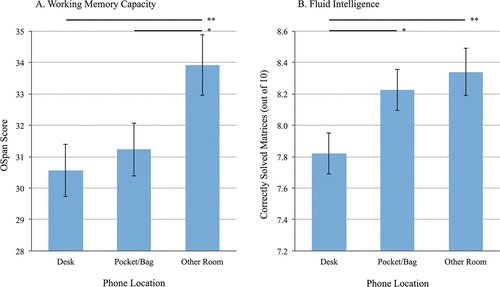
\includegraphics{img/braindrain1.jpg}

}

\caption{\label{fig-braindrain}Handy in Sichtweite verringert die
kognitiven Ressourcen}

\end{figure}%

\end{example}

\begin{exercise}[]\protect\hypertarget{exr-braindrain1}{}\label{exr-braindrain1}

Benennen Sie X und Y in Beispiel~\ref{exm-braindrain2}! \(\square\)

\end{exercise}

\begin{exercise}[]\protect\hypertarget{exr-braindrain-chatgpt}{}\label{exr-braindrain-chatgpt}

Fragen Sie einen Bot (z.B. ChatGPT) zum Stand der Forschung hinsichtlich
der Braindrain-Forschungsfrage. Diskutieren Sie die Antwort, auch in
ihren Grenzen. \(\square\)

\end{exercise}

\begin{tcolorbox}[enhanced jigsaw, colback=white, opacityback=0, arc=.35mm, titlerule=0mm, breakable, toptitle=1mm, colframe=quarto-callout-caution-color-frame, title=\textcolor{quarto-callout-caution-color}{\faFire}\hspace{0.5em}{Vorsicht}, rightrule=.15mm, colbacktitle=quarto-callout-caution-color!10!white, coltitle=black, leftrule=.75mm, bottomrule=.15mm, bottomtitle=1mm, opacitybacktitle=0.6, toprule=.15mm, left=2mm]

Es ist ein häufiger Fehler, in der Forschungsfrage zu formulieren ``X
führt zu Y'', aber in der Analyse keine Methode zu verwenden, die
geeignet ist, kausale Zusammenhänge aufzudecken. Es reicht nicht, dass
man z.B. einen (negativen) Zusammenhang zwischen der Häufigkeit von
Smartphone-Nutzung und Konzentrationsfähigkeit findet (Schwaiger \&
Tahir, 2022), um zu sagen: ``Daddeln macht dumm!''. Es könnte ja z.B.
auch umgekehrt sein. Platt gesagt: ``Dummheit führt zu Daddeln''.
Weitere Erklärungen sind möglich. Vorsicht also mit (vor)schnellen
Aussagen zu kausalen Abhängigkeiten.

\end{tcolorbox}

\subsection{Der Prozess der
Datenanalyse}\label{der-prozess-der-datenanalyse}

Datenanalyse ist eine Art des Problemlösens. Anders gesagt, man macht es
nicht zum Spaß\footnote{jedenfalls nicht alle von uns}, sondern um ein
Ziel zu erreichen, d.h. ein Problem zu lösen. Daher analysiert man nicht
gleich zu Anfang wild drauf los. Zunächst 1) klärt man das Problem und
das Ziel. Dann 2) plant man das Vorgehen, z.B. welche Daten man erheben
möchte. Als nächstes 3) erhebt man die Daten und bereitet sie auf.
Schließlich kann man sie 4) endlich analysieren. Aber Daten sprechen
nicht für sich, man muss sie 5) interpretieren und Schlüsse daraus
ziehen. Dazu gehört auch, dass man die Schwächen der eigenen Analyse
kritisch beleuchtet, vgl. Abbildung~\ref{fig-ppdac}. Diesen Ablauf nennt
man auch das PPDAC-Modell (MacKay \& Oldford, 2000):

\begin{itemize}
\tightlist
\item
  P: \emph{Problem} (Problem und Ziel und Sachgegenstand verstehen)
\item
  P: \emph{Plan} (Vorgehen planen)
\item
  D: \emph{Data} (Daten erheben und aufbereiten)
\item
  A: \emph{Analysis} (Daten analysieren)
\item
  C: \emph{Conclusions} (Schlussfolgerungen ziehen; Daten interpretieren
  )
\end{itemize}

\begin{figure}

\centering{

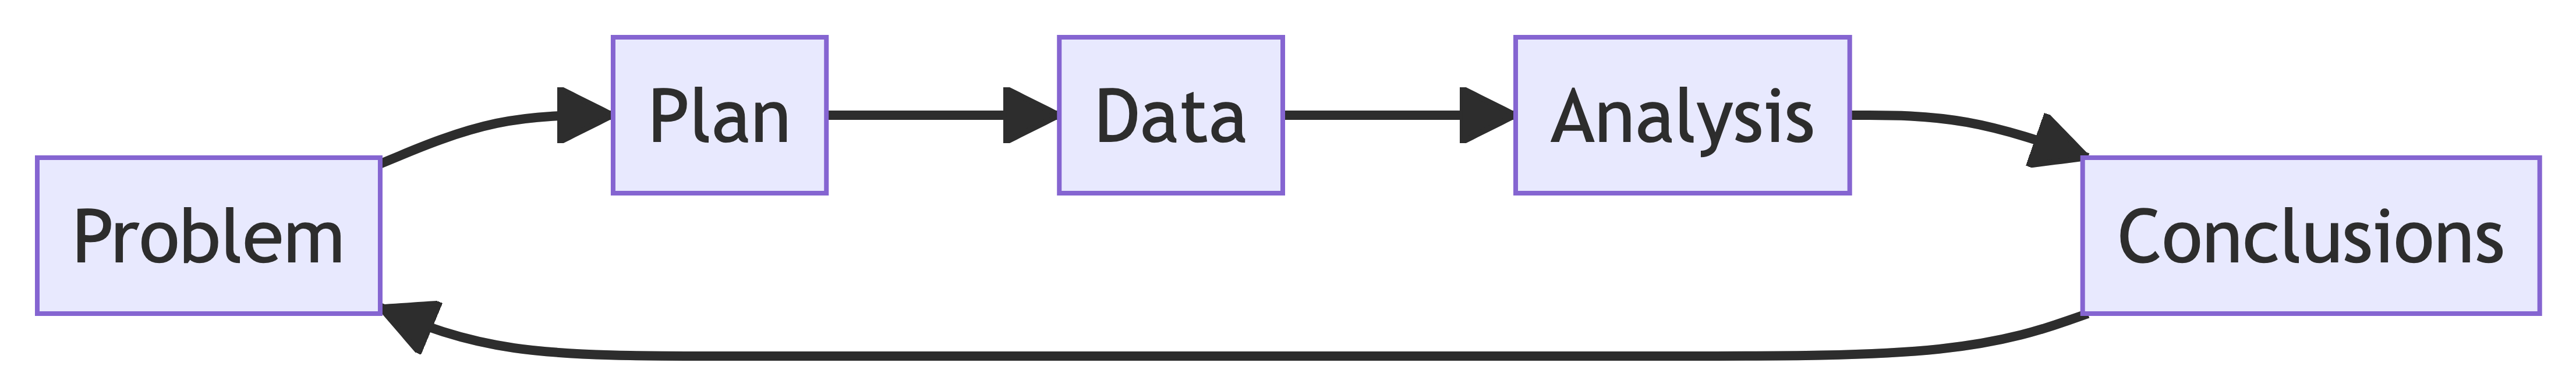
\includegraphics[width=5.76in,height=0.88in]{010-rahmen_files/figure-latex/mermaid-figure-4.png}

}

\caption{\label{fig-ppdac}Datenanalyse als Prozess: Das PPDAC-Modell}

\end{figure}%

\section{Was sind Daten?}\label{was-sind-daten}

\begin{definition}[Hallo,
Daten]\protect\hypertarget{def-daten}{}\label{def-daten}

Daten kann man als eine geordnete Folge von Zeichen
definieren.\(\square\)

\end{definition}

Daten kommen häufig in Tabellenform vor; so sind sie (oft) am besten zu
untersuchen, s. Tabelle~\ref{tbl-daten}.

\begin{longtable}{rlr}

\caption{\label{tbl-daten}So sehen Daten aus.}

\tabularnewline

\toprule
id & name & note \\ 
\midrule\addlinespace[2.5pt]
1 & Anna & 1.3 \\ 
2 & Berta & 2.3 \\ 
3 & Carla & 3.0 \\ 
\bottomrule

\end{longtable}

Die erste Spalte \texttt{id} ist nur eine laufende Nummer. Sie dient
dazu, die einzelnen Beobachtungen (hier Studentis) identifizieren zu
können und birgt ansonsten keine Information. Beispiele für ID-Variablen
sind z.B. Matrikulationsnummer, Personalausweisnummern oder
Bestellnummern.

\begin{example}[Daten zur Forschungsfrage
2]\protect\hypertarget{exm-daten}{}\label{exm-daten}

Hier ist ein Auszug der Daten zur Tabelle \texttt{mariokart}, s.
Tabelle~\ref{tbl-mariokart}.

\begin{longtable}[]{@{}
  >{\raggedleft\arraybackslash}p{(\columnwidth - 18\tabcolsep) * \real{0.1011}}
  >{\raggedleft\arraybackslash}p{(\columnwidth - 18\tabcolsep) * \real{0.0787}}
  >{\raggedright\arraybackslash}p{(\columnwidth - 18\tabcolsep) * \real{0.0562}}
  >{\raggedleft\arraybackslash}p{(\columnwidth - 18\tabcolsep) * \real{0.1011}}
  >{\raggedleft\arraybackslash}p{(\columnwidth - 18\tabcolsep) * \real{0.0899}}
  >{\raggedleft\arraybackslash}p{(\columnwidth - 18\tabcolsep) * \real{0.1011}}
  >{\raggedright\arraybackslash}p{(\columnwidth - 18\tabcolsep) * \real{0.1236}}
  >{\raggedleft\arraybackslash}p{(\columnwidth - 18\tabcolsep) * \real{0.1348}}
  >{\raggedright\arraybackslash}p{(\columnwidth - 18\tabcolsep) * \real{0.1348}}
  >{\raggedleft\arraybackslash}p{(\columnwidth - 18\tabcolsep) * \real{0.0787}}@{}}

\caption{\label{tbl-mariokart}Auszug aus der Tabelle mariokart}

\tabularnewline

\toprule\noalign{}
\begin{minipage}[b]{\linewidth}\raggedleft
duration
\end{minipage} & \begin{minipage}[b]{\linewidth}\raggedleft
n\_bids
\end{minipage} & \begin{minipage}[b]{\linewidth}\raggedright
cond
\end{minipage} & \begin{minipage}[b]{\linewidth}\raggedleft
start\_pr
\end{minipage} & \begin{minipage}[b]{\linewidth}\raggedleft
ship\_pr
\end{minipage} & \begin{minipage}[b]{\linewidth}\raggedleft
total\_pr
\end{minipage} & \begin{minipage}[b]{\linewidth}\raggedright
ship\_sp
\end{minipage} & \begin{minipage}[b]{\linewidth}\raggedleft
seller\_rate
\end{minipage} & \begin{minipage}[b]{\linewidth}\raggedright
stock\_photo
\end{minipage} & \begin{minipage}[b]{\linewidth}\raggedleft
wheels
\end{minipage} \\
\midrule\noalign{}
\endhead
\bottomrule\noalign{}
\endlastfoot
3 & 20 & new & 0.99 & 4.00 & 51.55 & standard & 1580 & yes & 1 \\
7 & 13 & used & 0.99 & 3.99 & 37.04 & firstClass & 365 & yes & 1 \\
3 & 16 & new & 0.99 & 3.50 & 45.50 & firstClass & 998 & no & 1 \\
3 & 18 & new & 0.99 & 0.00 & 44.00 & standard & 7 & yes & 1 \\
1 & 20 & new & 0.01 & 0.00 & 71.00 & media & 820 & yes & 2 \\
3 & 19 & new & 0.99 & 4.00 & 45.00 & standard & 270144 & yes & 0 \\

\end{longtable}

Eine Erklärung aller Variablen des Datensatzes \texttt{mariokart} findet
sich
\href{https://www.openintro.org/data/index.php?data=mariokart}{hier}.
\(\square\)

\end{example}

\begin{definition}[Data
Dictionary]\protect\hypertarget{def-datadict}{}\label{def-datadict}

Eine Erklärung, was die Namen einer Datentabelle bedeuten, nennt man
\emph{Code Book} or \emph{Data Dictionary}.\(\square\)

\end{definition}

\subsection{Was ist eine Variable?}\label{was-ist-eine-variable}

\begin{definition}[Variable]\protect\hypertarget{def-var}{}\label{def-var}

Eine Variable ist ein Platzhalter, der für ein Merkmal steht, das
verschiedene Werte annehmen kann.\(\square\)

\end{definition}

Man kann sich eine Variable wie einen Behälter vorstellen, auf dem mit
einem Stift geschrieben steht, was für eine Art Inhalt darin ist, s.
Abbildung~\ref{fig-var-zuweisen}.

\begin{figure}

\centering{

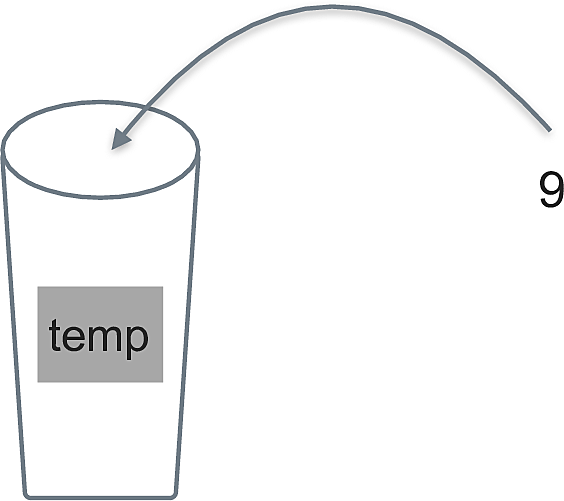
\includegraphics[width=0.25\textwidth,height=\textheight]{img/Variablen_zuweisen.png}

}

\caption{\label{fig-var-zuweisen}Wir definieren eine Variable ``temp''
mit dem Inhalt ``9''}

\end{figure}%

\subsection{Beobachtungseinheit}\label{beobachtungseinheit}

\begin{definition}[Beobachtungseinheit]\protect\hypertarget{def-beobeinheit}{}\label{def-beobeinheit}

Beobachtungseinheiten sind die Dinge, die wir untersuchen (beobachten).
Beobachtungseinheiten sind die Träger von Variablen.\(\square\)

\end{definition}

In Tabelle~\ref{tbl-daten} gibt es drei Variablen: \texttt{id},
\texttt{Name} und \texttt{Note}. Es gibt auch drei
Beobachtungseinheiten: \emph{Anna}, \emph{Berta} und \emph{Carla.}

\subsection{Wert}\label{wert}

\begin{definition}[Wert]\protect\hypertarget{def-wert}{}\label{def-wert}

Ein \emph{Wert} ist der Inhalt einer Variablen.\(\square\)

\end{definition}

In Abbildung~\ref{fig-var-zuweisen} ist der Wert von \texttt{temp} 9. In
Tabelle~\ref{tbl-daten} hat die Variable \texttt{name} drei Elemente:
Anna, Berta, Carla. Der Wert des 2. Elements ist Berta.

\begin{definition}[]\protect\hypertarget{def-auspraegung}{}\label{def-auspraegung}

Als \emph{Ausprägungen} bezeichnet man die verschiedenen Werte einer
Variablen. \(\square\)

\end{definition}

\begin{example}[]\protect\hypertarget{exm-geschlecht}{}\label{exm-geschlecht}

In einer Studie wurden zehn Probanden untersucht. Die Variable
\texttt{geschlecht} dokumentiert die Geschlechter der Personen:

\begin{Shaded}
\begin{Highlighting}[]
\NormalTok{geschlecht }\OtherTok{\textless{}{-}} \FunctionTok{c}\NormalTok{(}\StringTok{"Mann"}\NormalTok{, }\StringTok{"Frau"}\NormalTok{, }\StringTok{"Frau"}\NormalTok{, }\StringTok{"Frau"}\NormalTok{, }\StringTok{"Mann"}\NormalTok{,}
                \StringTok{"Frau"}\NormalTok{, }\StringTok{"Mann"}\NormalTok{, }\StringTok{"Mann"}\NormalTok{, }\StringTok{"divers"}\NormalTok{, }\StringTok{"Frau"}\NormalTok{)}
\NormalTok{geschlecht}
\DocumentationTok{\#\#  [1] "Mann"   "Frau"   "Frau"   "Frau"   "Mann"   "Frau"   "Mann"   "Mann"  }
\DocumentationTok{\#\#  [9] "divers" "Frau"}
\end{Highlighting}
\end{Shaded}

In dieser Variable (die aus 10 Werten besteht) finden sich drei
Ausprägungen: divers, Frau, Mann.\(\square\)

\end{example}

\begin{tcolorbox}[enhanced jigsaw, colback=white, opacityback=0, arc=.35mm, titlerule=0mm, breakable, toptitle=1mm, colframe=quarto-callout-tip-color-frame, title=\textcolor{quarto-callout-tip-color}{\faLightbulb}\hspace{0.5em}{Tipp}, rightrule=.15mm, colbacktitle=quarto-callout-tip-color!10!white, coltitle=black, leftrule=.75mm, bottomrule=.15mm, bottomtitle=1mm, opacitybacktitle=0.6, toprule=.15mm, left=2mm]

Gerade haben Sie etwas Computer-Syntax gesehen, genauer gesagt, Befehle
aus der Programmiersprache \emph{R}. Bisher haben wir diese Befehle
nicht kennengelernt. Sie verstehen Sie vermutlich (nicht ganz).
Ignorieren Sie diese Befehle einfach erstmal.

\end{tcolorbox}

\subsection{Tidy-Data}\label{tidy-data}

\begin{definition}[]\protect\hypertarget{def-tidy}{}\label{def-tidy}

Unter \emph{Tidy-Data} (tidy data, ``Normalform'') versteht man eine
Tabelle, in der jede Zeile eine Beobachtungseinheit darstellt, jede
Spalte eine Variable und jede Zelle der Tabelle einen Wert, s.
Abbildung~\ref{fig-tidy1}. (Zusätzlich ist noch eine ``Kopfzeile''
erlaubt, in der die Namen der Variablen stehen.)\(\square\)

\end{definition}

Tabelle~\ref{tbl-daten} ist ein Beispiel für Tidy-Data.
Abbildung~\ref{fig-tidy1} zeigt ein Sinnbild für Tidy-Data (Wickham \&
Grolemund, 2018). Und Abbildung~\ref{fig-tidy-hadley} erläutert das
Tidy-Prinzip genauer.

\begin{figure}

\begin{minipage}{0.50\linewidth}

\centering{

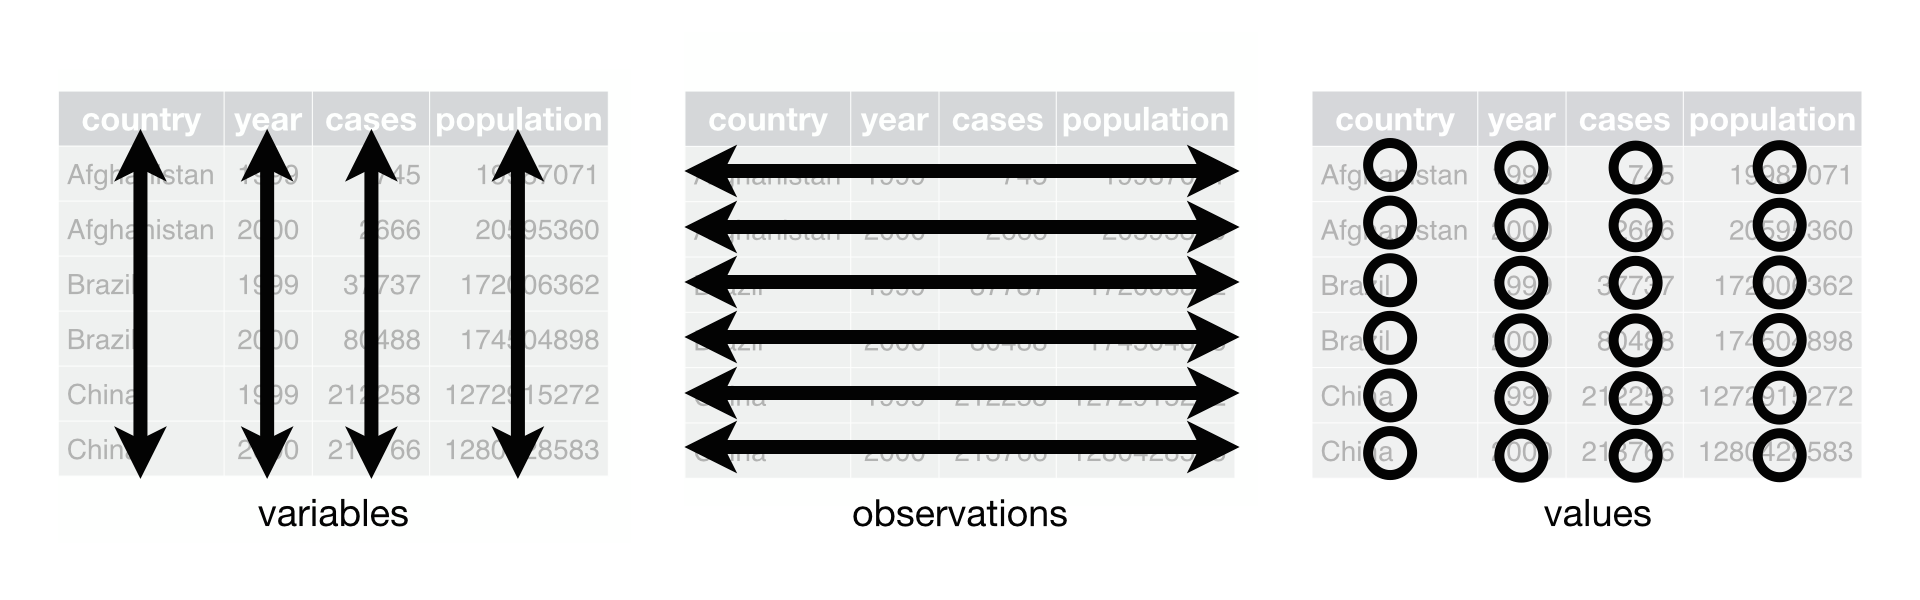
\includegraphics{img/tidy-1.png}

}

\subcaption{\label{fig-tidy1}Tidy-Data-Sinnbild. Image Credit: Hadley
Wickham}

\end{minipage}%
%
\begin{minipage}{0.50\linewidth}

\centering{

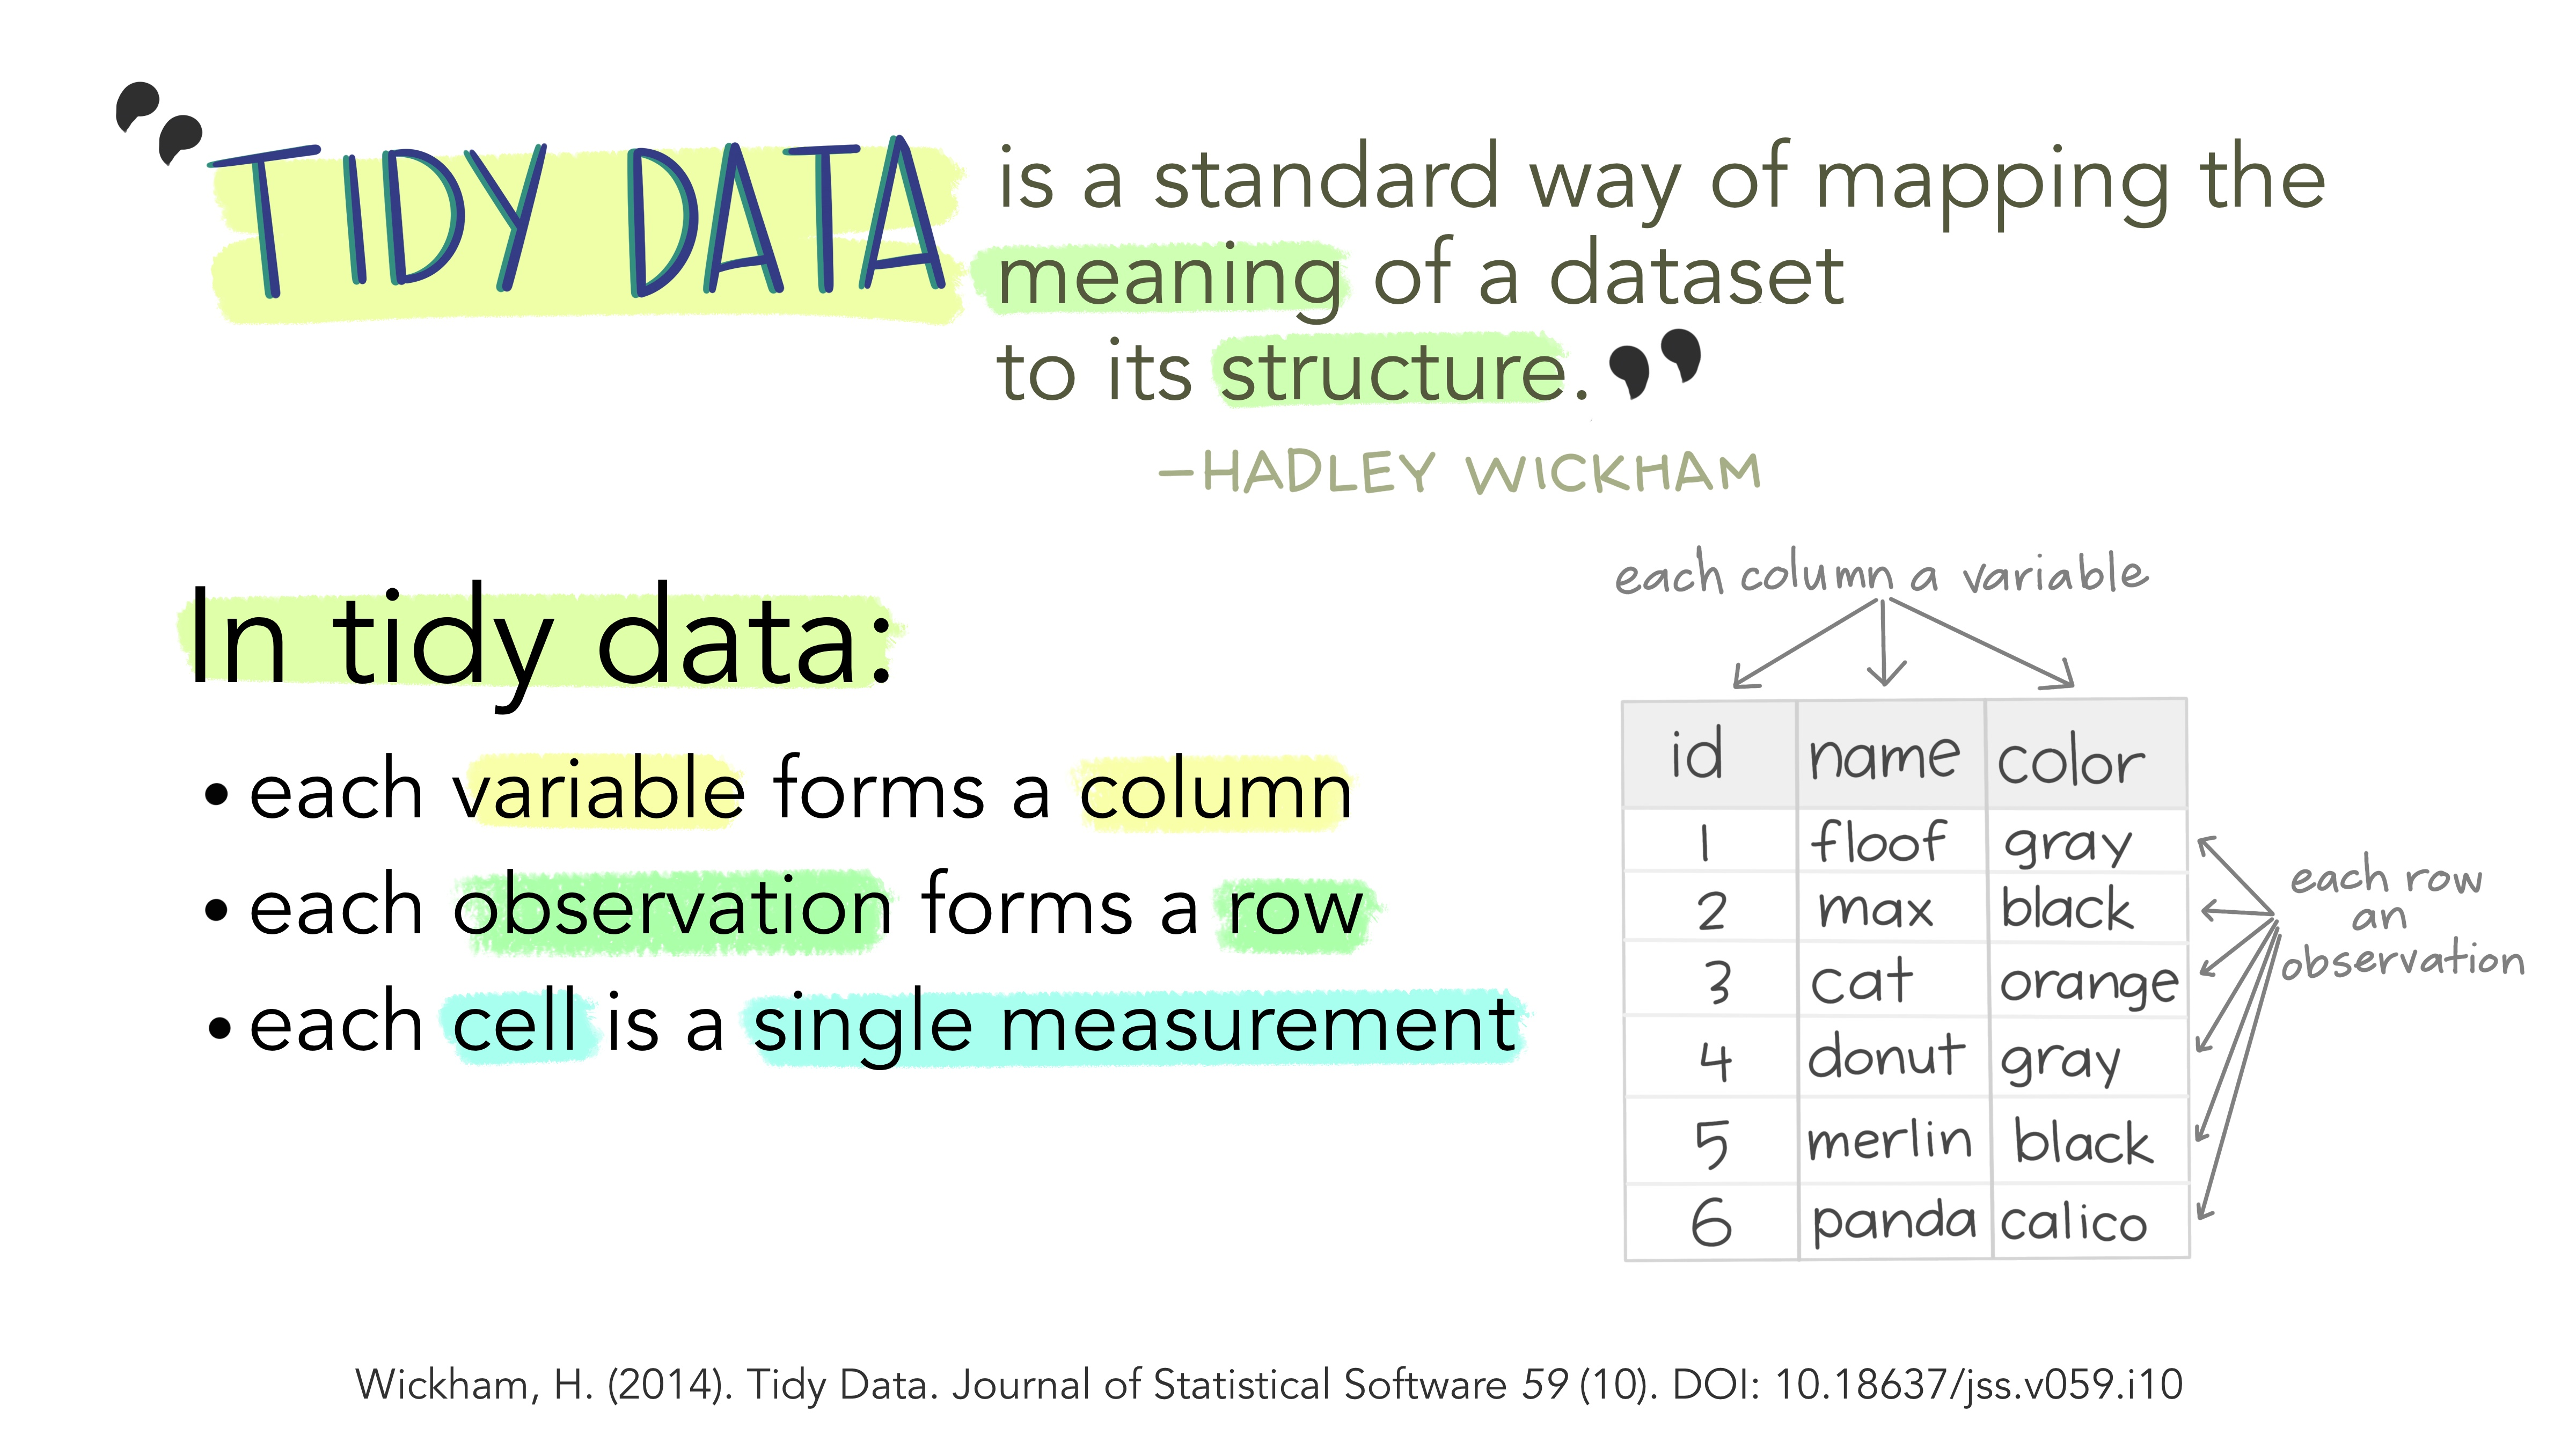
\includegraphics{img/tidydata_1.jpg}

}

\subcaption{\label{fig-tidy-hadley}Was ist Tidy-Data?. Image Credit:
Allision Horst}

\end{minipage}%

\caption{\label{fig-tidy-all}Stay Tidy!}

\end{figure}%

\begin{tcolorbox}[enhanced jigsaw, colback=white, opacityback=0, arc=.35mm, titlerule=0mm, breakable, toptitle=1mm, colframe=quarto-callout-important-color-frame, title=\textcolor{quarto-callout-important-color}{\faExclamation}\hspace{0.5em}{Wichtig}, rightrule=.15mm, colbacktitle=quarto-callout-important-color!10!white, coltitle=black, leftrule=.75mm, bottomrule=.15mm, bottomtitle=1mm, opacitybacktitle=0.6, toprule=.15mm, left=2mm]

Für eine statistische Analyse ist es oft sinnvoll, dass die Daten im
Tidy-Format vorliegen.

\end{tcolorbox}

Der Vorteil des Tidy-Formats ist es, dass man weiß, wie die Daten
aufgebaut sind. Außerdem können Statistikprogramme oft mit dieser Form
am besten umgehen, s. Abbildung~\ref{fig-tidy3}.

\begin{figure}

\centering{

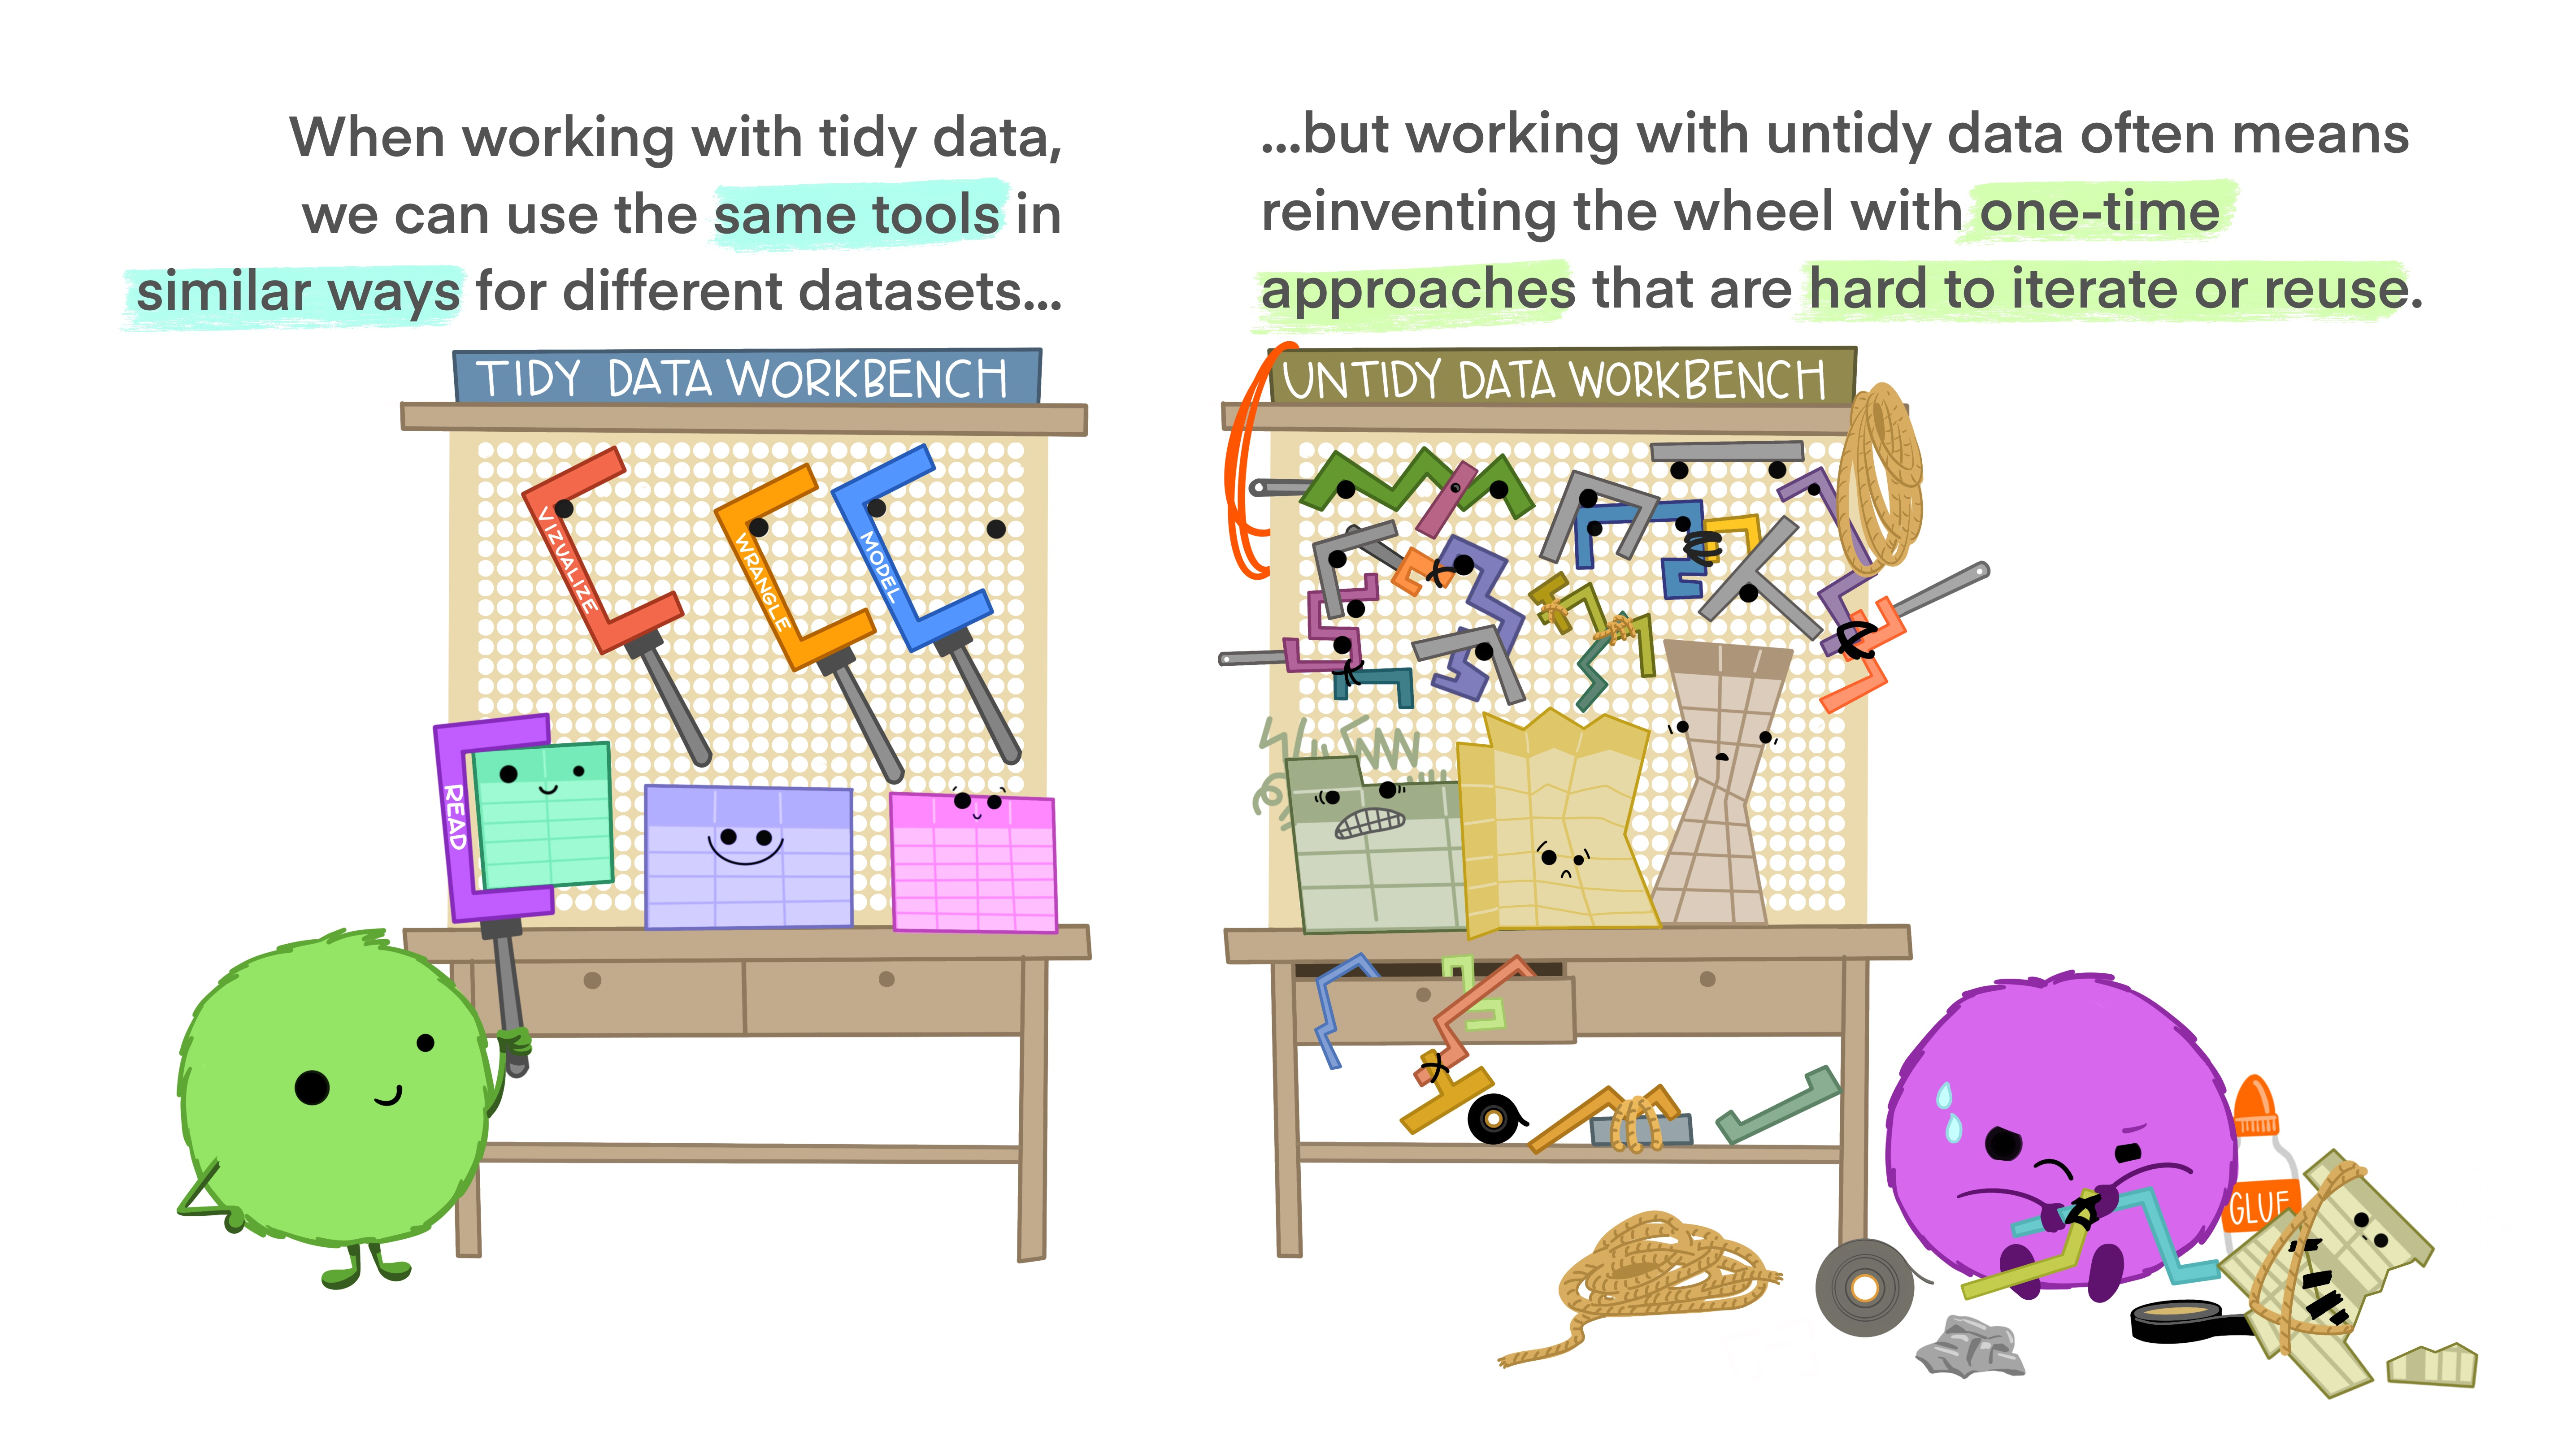
\includegraphics[width=0.75\textwidth,height=\textheight]{img/tidydata_3.jpg}

}

\caption{\label{fig-tidy3}Immer schön Ordnung halten\ldots{} Image
credit: Allision Horst}

\end{figure}%

\href{https://github.com/allisonhorst/stats-illustrations}{Quelle}

Das Tidy-Format wird auch als ``langes'' Format bezeichnet.

Abbildung~\ref{fig-long-wide-anim} zeigt einen Datensatz in der
``langen'' Form, also tidy, und den gleichen Datensatz, umformatiert in
der ``breiten'' Form, nicht-tidy.

\begin{figure}

\centering{

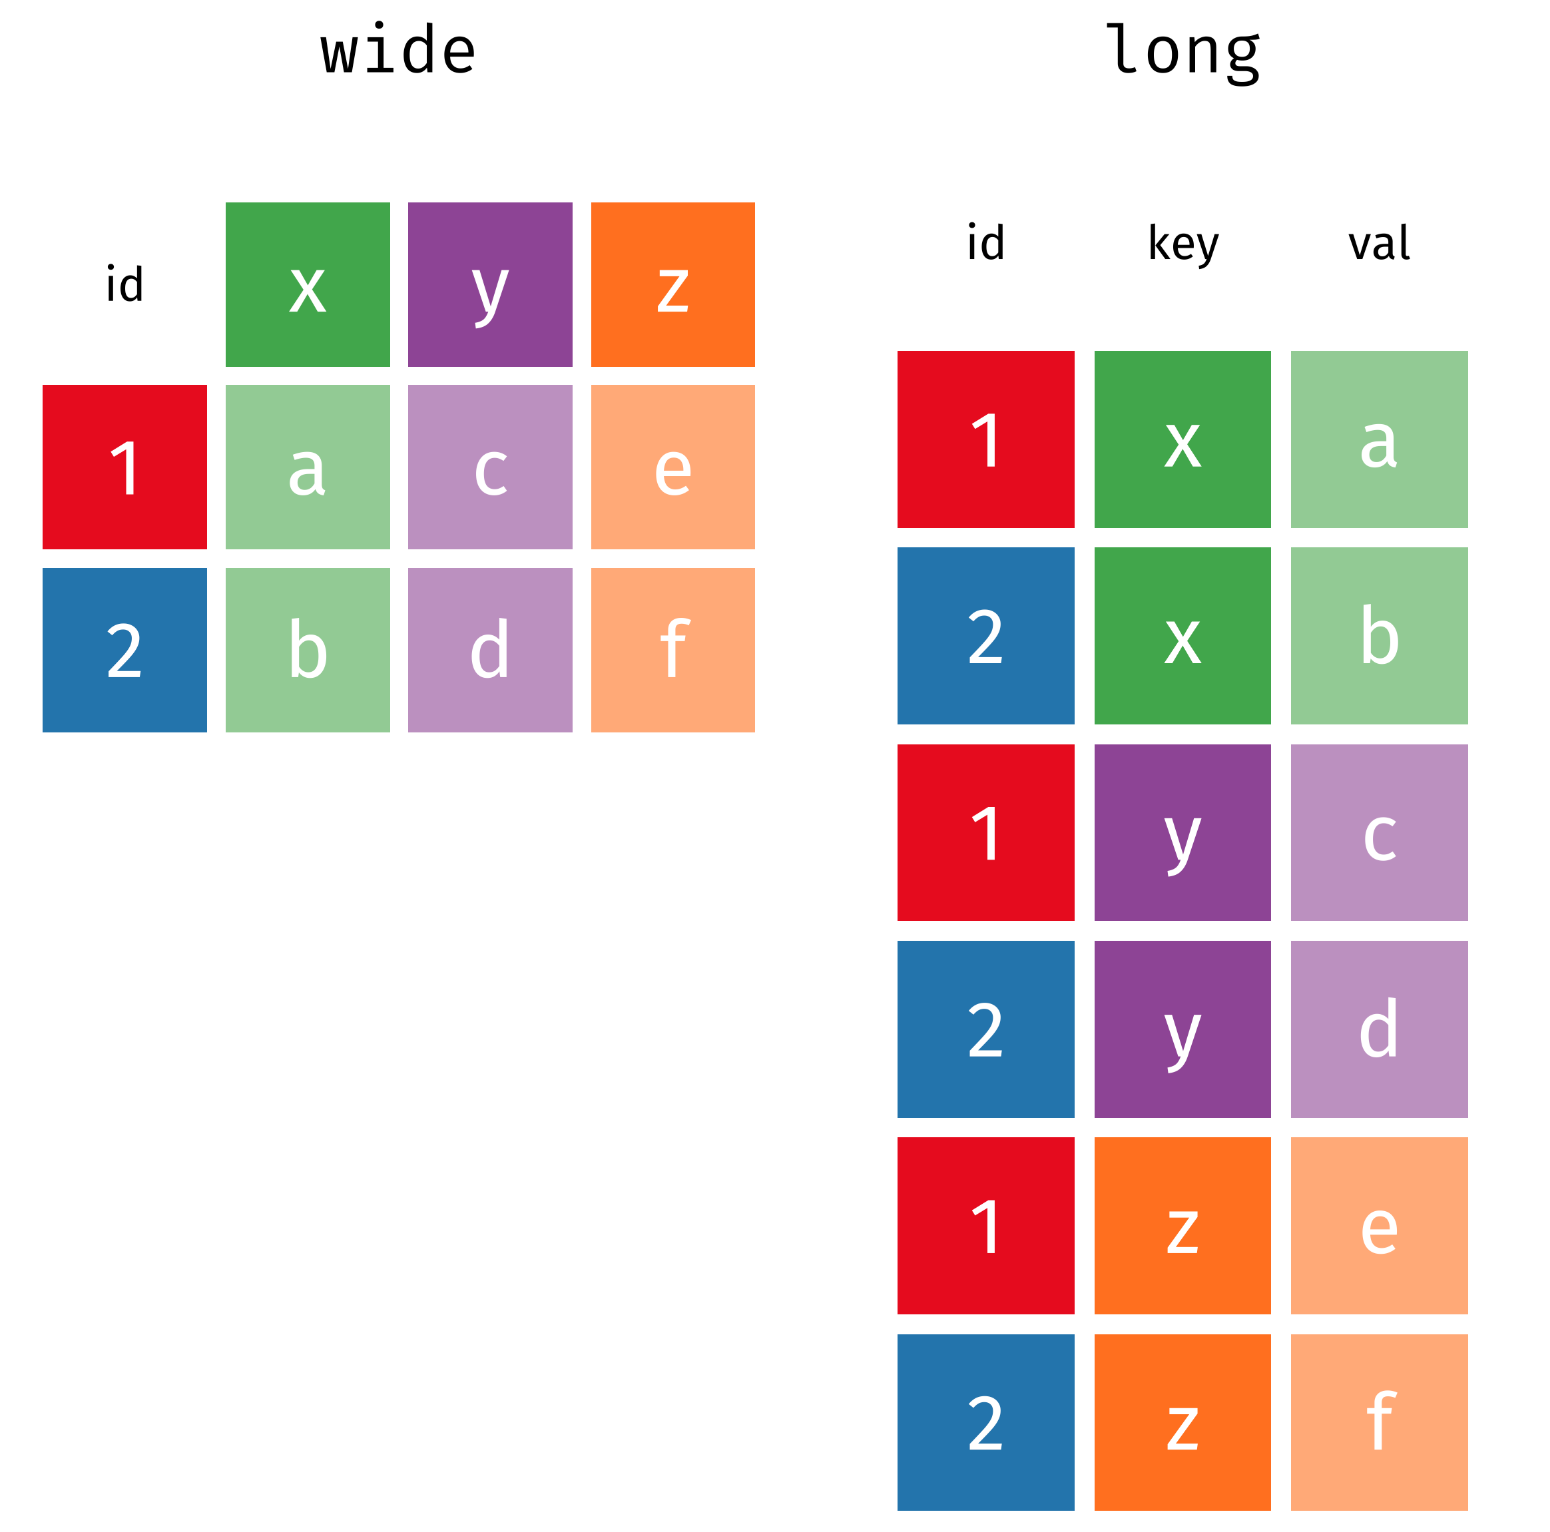
\includegraphics[width=0.5\textwidth,height=\textheight]{img/wide-long.png}

}

\caption{\label{fig-long-wide-anim}Links: Eine Tabelle mit Format
``wide'' - nicht ``tidy''. Rechts: Das ``Langformat'' (``long'') ist
``tidy''.}

\end{figure}%

{Quelle: Garrick Aden-Buie, 2018, CC0-1.0 license,
\url{https://www.garrickadenbuie.com/project/tidyexplain/}}

\begin{example}[]\protect\hypertarget{exm-widelong}{}\label{exm-widelong}

Im Folgenden sind eine Nicht-Tidy-Tabelle (Tabelle~\ref{tbl-untidy1})
und eine Tidy-Tablle (Tabelle~\ref{tbl-tidy1}) dargestellt.

\begin{figure}

\begin{minipage}{0.50\linewidth}

\subsubsection{Breitformat}\label{breitformat}

\begin{longtable}[]{@{}lrrr@{}}

\caption{\label{tbl-untidy1}Beispiel für eine NICHT-Tidy-Tabelle
(Breitformat)}

\tabularnewline

\toprule\noalign{}
Produkt & Umsatz\_2021 & Umsatz\_2022 & Umsatz\_2023 \\
\midrule\noalign{}
\endhead
\bottomrule\noalign{}
\endlastfoot
Hammer & 10 & 11 & 12 \\
Nägel & 15 & 10 & 5 \\

\end{longtable}

\end{minipage}%
%
\begin{minipage}{0.50\linewidth}

\subsubsection{Langformat (tidy)}\label{langformat-tidy}

\begin{longtable}[]{@{}llr@{}}

\caption{\label{tbl-tidy1}Beispiel für eine Tidy-Tabelle (Langformat)}

\tabularnewline

\toprule\noalign{}
Produkt & Jahr & Umsatz \\
\midrule\noalign{}
\endhead
\bottomrule\noalign{}
\endlastfoot
Hammer & 2021 & 10 \\
Hammer & 2022 & 11 \\
Hammer & 2023 & 12 \\
Nägel & 2021 & 15 \\
Nägel & 2022 & 10 \\
Nägel & 2023 & 5 \\

\end{longtable}

\end{minipage}%

\end{figure}%

\end{example}

\begin{exercise}[]\protect\hypertarget{exr-widelong}{}\label{exr-widelong}

Suchen Sie ein Beispiel für eine Konfiguration einer Tabelle im Long-
vs.~Wide-Format. \(\square\)

\end{exercise}

\begin{quote}
🧑‍🎓 Wozu braucht man das Tidy-Format?
\end{quote}

\begin{quote}
👩‍🏫 In vielen Software-Programmen der Datenanalyse weißt man z.B. der X-
oder Y-Variable eine Spalte einer Tabelle zu. Möchte man etwa die
Veränderung des Umsatzes im Verlauf der Jahre visualisieren oder
analysieren, so braucht es die Spalten `Jahr' und `Umsatz', also ein
Tidy-Format.
\end{quote}

\begin{figure}

\centering{

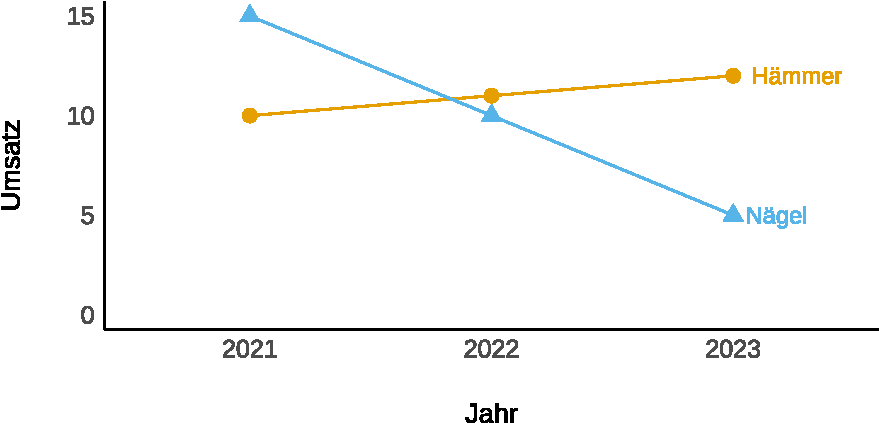
\includegraphics{010-rahmen_files/figure-pdf/fig-tidy-1.pdf}

}

\caption{\label{fig-tidy}Beispiel für eine Visualisierung auf Basis
einer Tidy-Tabelle, vgl. Tabelle~\ref{tbl-tidy1}}

\end{figure}%

\subsection{Je mehr, desto besser (?)}\label{je-mehr-desto-besser}

Was Daten betrifft, könnte man behaupten: ``Viel hilft viel'' oder ``Je
mehr, desto besser''. Natürlich unter sonst gleichen
Umständen\footnote{Ceteris paribus, auf Latein, hört sich gleich viel
  schlauer an}. Viel Datenmüll ist natürlich nicht besser als ein paar
knappe, wasserdichte Fakten!

\begin{example}[]\protect\hypertarget{exm-samplesize}{}\label{exm-samplesize}

Um Ihre eigene Lehraktivität zu organisieren, wollen Sie sich ein Bild
machen, wie viel Ihre Nebensitzer im Hörsaal so lernen. Sie blicken nach
links und fragen ``wie viel lernst du so?''. Sie blicken nach recht und
wiederholen die Frage gerichtet an den rechtsnebensitzenden
Kommilitonen. Dann addieren Sie die zwei Zahlen (unter der Annahme, dass
Sie zwei Zahlen bekommen haben), und teilen durch zwei, um den
Mittelwert zu erhalten.

Ein kritischer Geist könnte anmerken, dass Sie besser die Untersuchung
nicht gemacht hätten (auch wenn Sie, vielleicht ohne zu wollen, eine
statistische Untersuchung angestellt haben). Denn bei so wenig befragten
Personen ist die Ungenauigkeit Ihrer Schätzung der typischen Lernzeit
bei Studentis einfach zu hoch.\(\square\)

\end{example}

Abbildung~\ref{fig-sample-estimate} veranschaulicht, dass man einen
Mittelwert genauer schätzen kann, wenn man auf eine größere Stichprobe
zurückgreift. Das Teilbild links zeigt den Mittelwert einer Stichprobe
mit \(n=20\) Beobachtungen. Das Teilbild rechts zeigt den Mittelwert
einer Stichprobe mit \(n=200\) Beobachtungen (jeweils aus der gleichen
Grundgesamtheit). Wie man sieht, ist im linken Teilbild die Streuung
(Variation) höher als im rechten Teilbild:

\begin{verbatim}
## $x
## [1] "Nummer der Stichprobe"
## 
## $y
## [1] "Wert"
## 
## attr(,"class")
## [1] "labels"
\end{verbatim}

\begin{figure}

\centering{

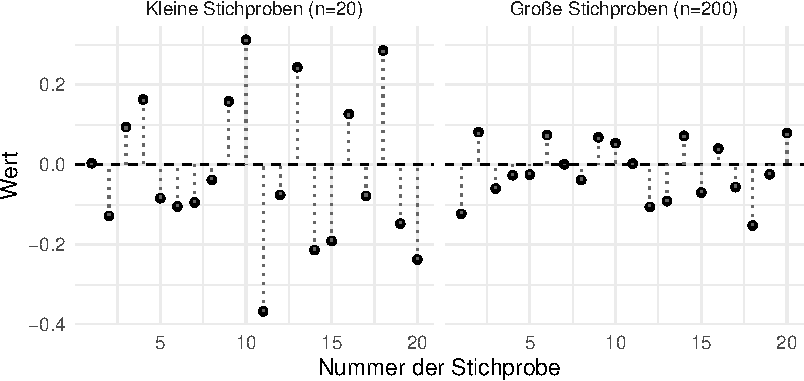
\includegraphics{010-rahmen_files/figure-pdf/fig-sample-estimate-1.pdf}

}

\caption{\label{fig-sample-estimate}Schätzgenauigkeit als Funktion der
Stichprobengröße}

\end{figure}%

Bildquelle: Karsten Lübke

\begin{tcolorbox}[enhanced jigsaw, colback=white, opacityback=0, arc=.35mm, titlerule=0mm, breakable, toptitle=1mm, colframe=quarto-callout-important-color-frame, title=\textcolor{quarto-callout-important-color}{\faExclamation}\hspace{0.5em}{Wichtig}, rightrule=.15mm, colbacktitle=quarto-callout-important-color!10!white, coltitle=black, leftrule=.75mm, bottomrule=.15mm, bottomtitle=1mm, opacitybacktitle=0.6, toprule=.15mm, left=2mm]

Mehr Daten = genauere Ergebnisse (unter sonst gleichen Umständen)
\(\square\)

\end{tcolorbox}

\begin{exercise}[Live-Experiment zum Effekt der
Stichprobengröße]\protect\hypertarget{exr-kleine-grosse-stipro}{}\label{exr-kleine-grosse-stipro}

In diesem Live-Experiment untersuchen wir den Effekt der
\emph{Stichprobengröße} auf die Streuung des Mittelwerts in der
\emph{Stichprobe.} Streuen die Ergebnisse mehr in kleinen Stichproben
als in großen? Probieren wir es aus!

In diesem Experiment werfen Sie (in kleinen Gruppen) eine Münze (auf
faire Art und Weise) und notieren das Ergebnis (Kopf oder Zahl). Uns
interessiert dabei die Frage, ob die Ergebnisse bei kleinen Stichproben
(n=5 Münzwürfe) anders streuen als in großen Stichproben (n=20
Münzwürfe).

Sie brauchen nur experimentierfreudige Partner (Kleingruppen mit 2-4
Personen), eine faire Münze und dann kann's los gehen!
\href{https://docs.google.com/forms/d/e/1FAIpQLSeAwqNyZtyQwttq5JrQdQ2AO7w5vzcVDXjiejKnyFNxiWtEag/viewform?usp=sf_link}{Klicken
Sie hier, um mit dem Experiment zu starten}

Die Daten aller Versuche können Sie
\href{https://docs.google.com/spreadsheets/d/11mKFFpr-Y1CMPpq4dGA-JA_Z9jRkPbXolo54Y0G_2gE/edit?usp=sharing}{hier}
einsehen. \(\square\)

\end{exercise}

\begin{example}[Dorfschulen machen die schlauesten
Schüler!]\protect\hypertarget{exm-schule-samplesize}{}\label{exm-schule-samplesize}

In einer Pressemitteilung sei zu lesen, dass die besten Schüler in den
Dorfschulen zu finden seien\footnote{Das ist eine fiktive Geschichte}.
Mit etwas Recherche finden Sie heraus, dass diese Aussage für
belastbaren Daten beruht: Tatsächlich sind die Notendurchschnitte auf
den kleinen Dorfschulen deutlich besser als in den großen Schulen in der
Stadt. Also stimmt die Behauptung der Pressemitteilung? Die gute
Landluft lässt das Hirn wachsen? Sie recherchieren noch etwas weiter in
den Daten. Dann fällt Ihnen auf: Die \emph{schlechtesten} Schüler kommen
auch aus den Dorfschulen! Eine statistische Erklärung bietet sich an: In
den Dorfschulen gibt es nur wenig Kinder und kleine Klassen -- die
Stichproben sind also klein. Bei kleinen Stichproben gibt es viel
Variation um den Mittelwert herum, s.
Abbildung~\ref{fig-sample-estimate}, und zwar nach oben (guter
Notenschnitt) und nach unten (schlechter Notenschnitt). \(\square\)

\end{example}

\section{Arten von Variablen}\label{sec-arten-variablen}

\subsection{Nach Position in der
Forschungsfrage}\label{nach-position-in-der-forschungsfrage}

Angenommen, Ihre Forschungsfrage lautet:

\begin{quote}
Hat Lernen einen Einfluss auf den Prüfungserfolg?
\end{quote}

In dem Fall gilt:

\begin{itemize}
\tightlist
\item
  \emph{Lernen} ist die Inputvariable/X-Variable/Ursache/unabhängig
  Variable (UV)
\item
  \emph{Prüfungserfolg} ist die
  Outputvariable/Y-Variable/Wirkung/abhängige Variable (AV)
\end{itemize}

Abbildung~\ref{fig-ueberblick-fragen} stellt diese beiden ``Positionen''
einer Variable dar. Die erste Position ist vor dem Pfeil. Die zweite
Position ist nach dem Pfeil.

\begin{figure}

\centering{

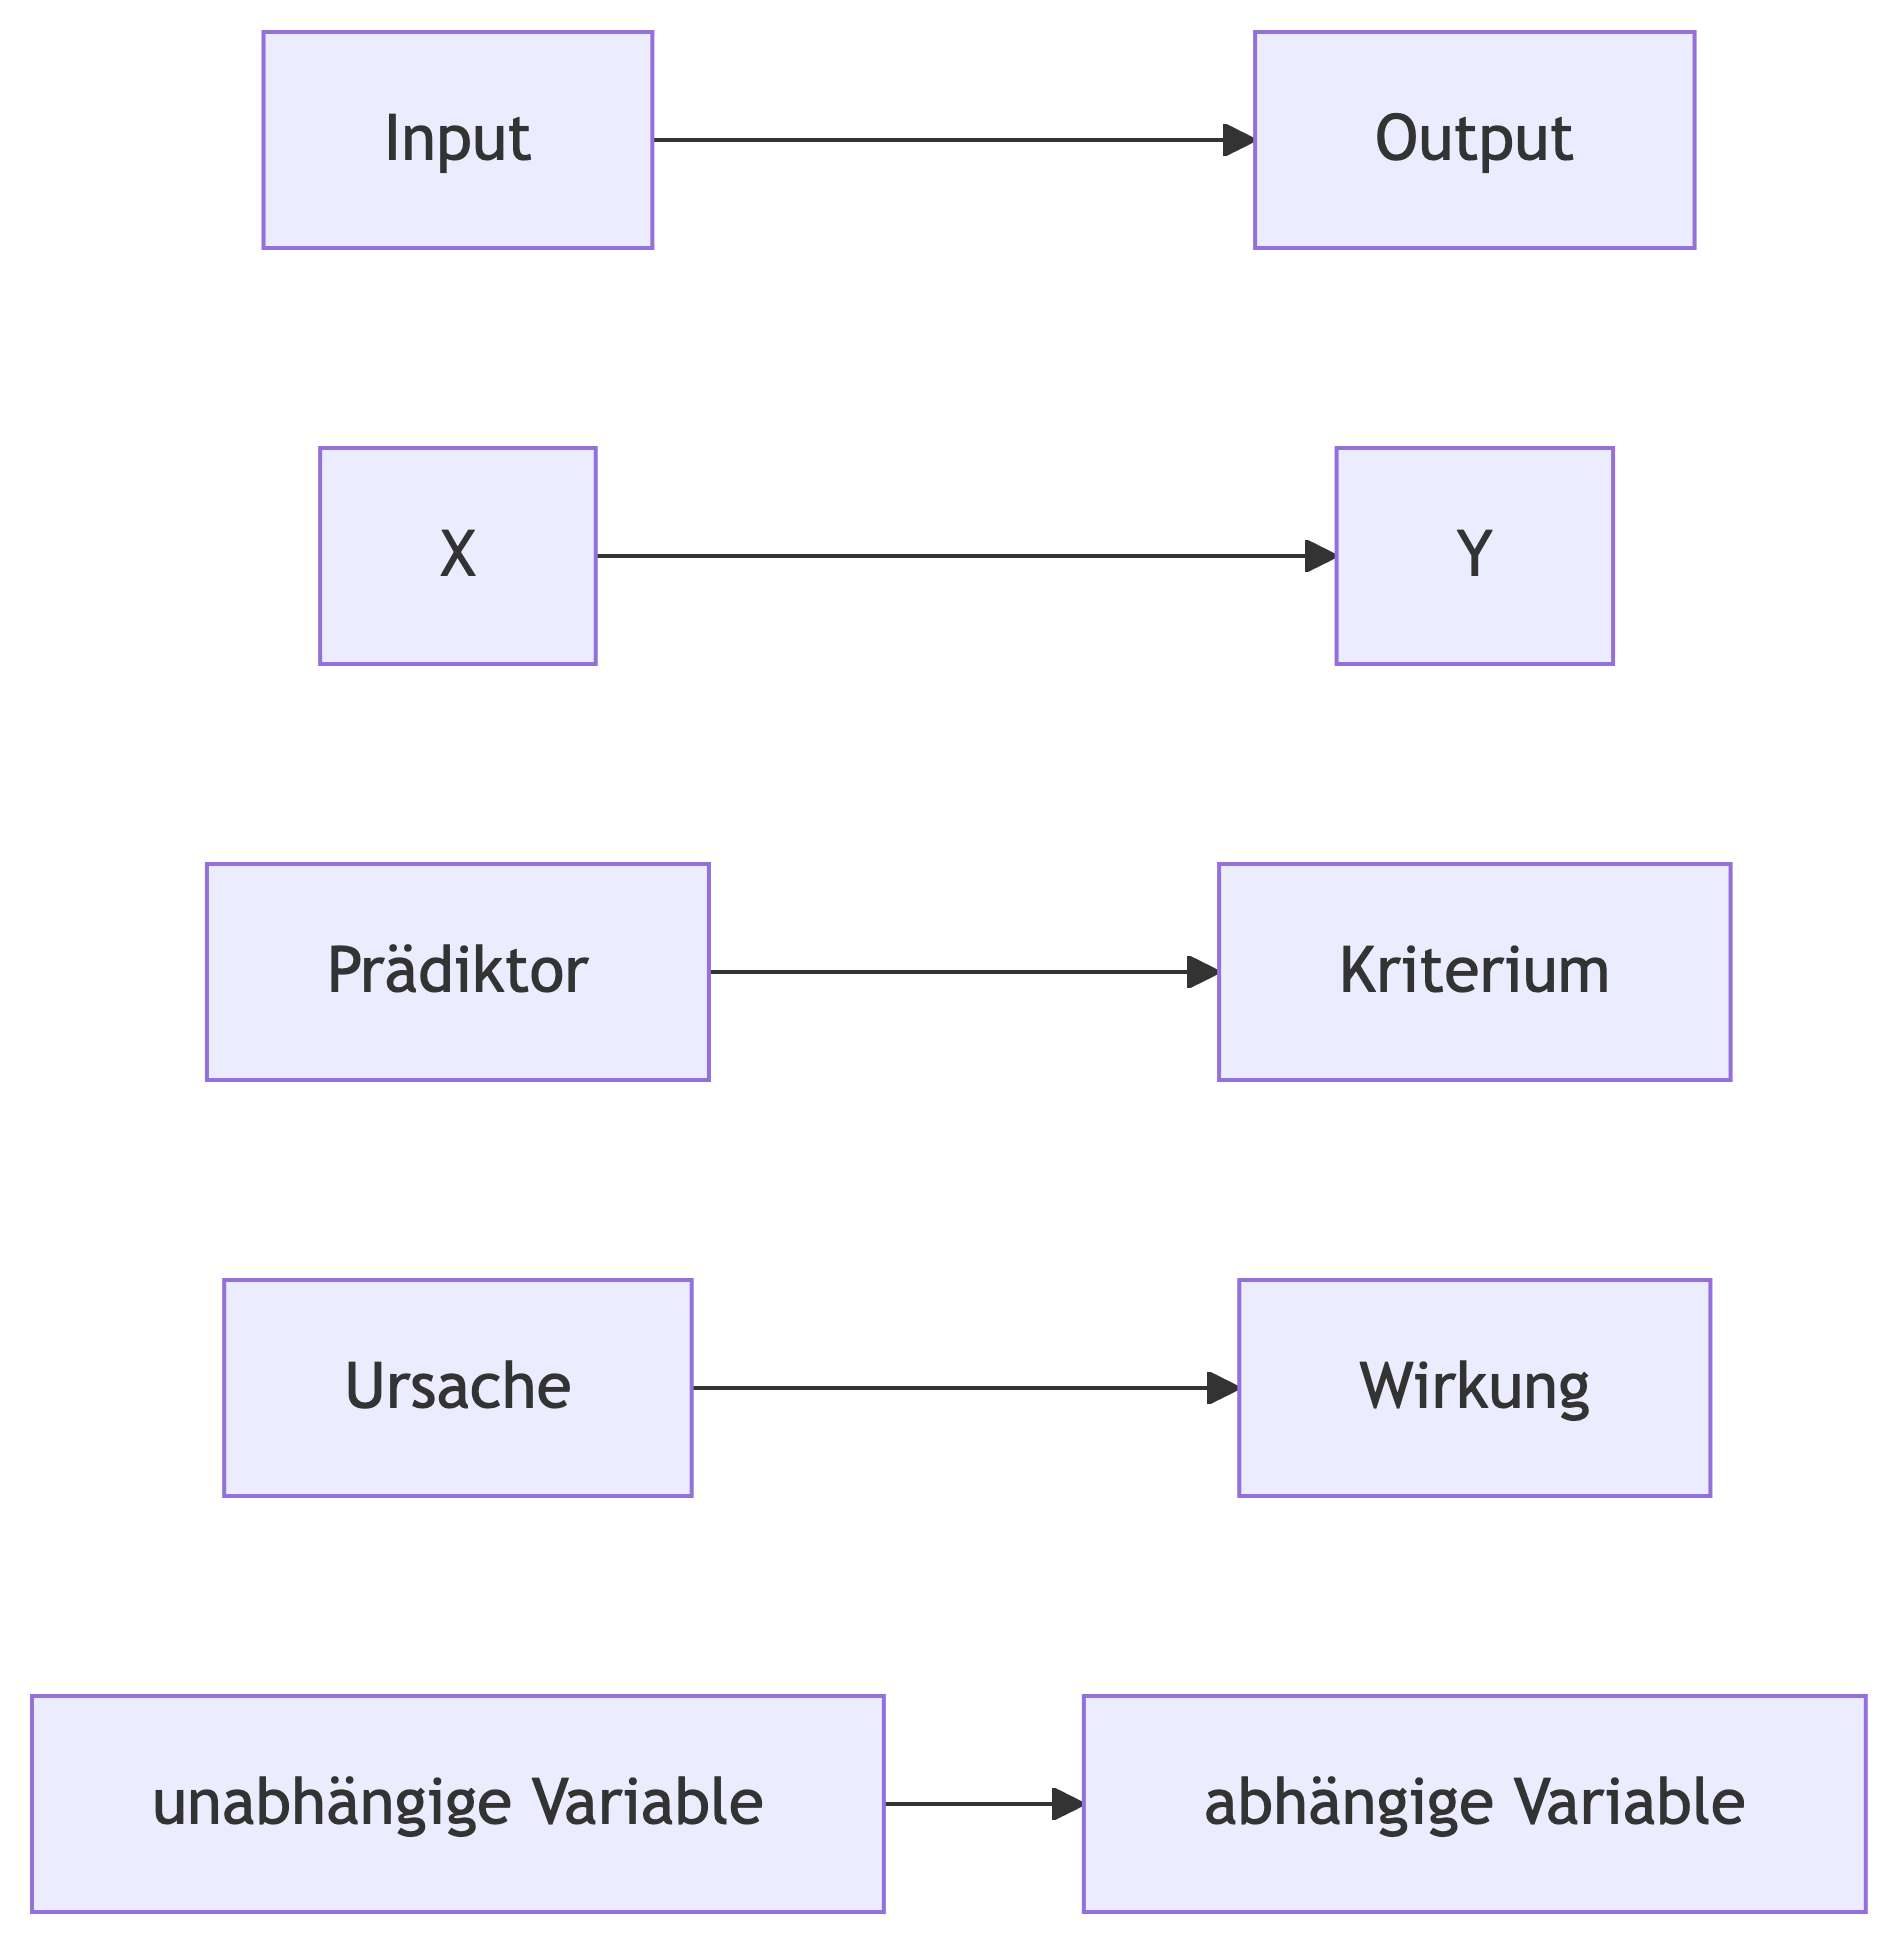
\includegraphics[width=4in,height=3.99in]{010-rahmen_files/figure-latex/mermaid-figure-3.png}

}

\caption{\label{fig-ueberblick-fragen}Synonyme Bezeichnungen für Input-
und Output-Variablen einer Forschungsfrage}

\end{figure}%

\begin{exercise}[]\protect\hypertarget{exr-uvav}{}\label{exr-uvav}

Überlegen Sie sich eine Forschungsfrage, die eine UV und eine AV
enthält. Sagen Sie einer/em Kommilitonen diese Forschungsfrage und
fragen Sie, was die UV und die AV ist. Bei richtiger Antwort belohnen
Sie großzügig. \(\square\)

\end{exercise}

\subsection{Nach dem Skalenniveau}\label{nach-dem-skalenniveau}

\begin{definition}[]\protect\hypertarget{def-skalenniveau}{}\label{def-skalenniveau}

Der Begriff \emph{Skalenniveau} wird verwendet, um die Art und Menge der
Information, die in Variablen enthalten ist, zu benennen. Diese
Klassifikation basiert auf den Eigenschaften der Daten und den
mathematischen Operationen, die sinnvoll auf diese Daten angewendet
werden können. \(\square\)

\end{definition}

Abbildung~\ref{fig-skalenniveau} gibt einen Überblick über typisch
verwendete Skalenniveaus.

\begin{figure}

\centering{

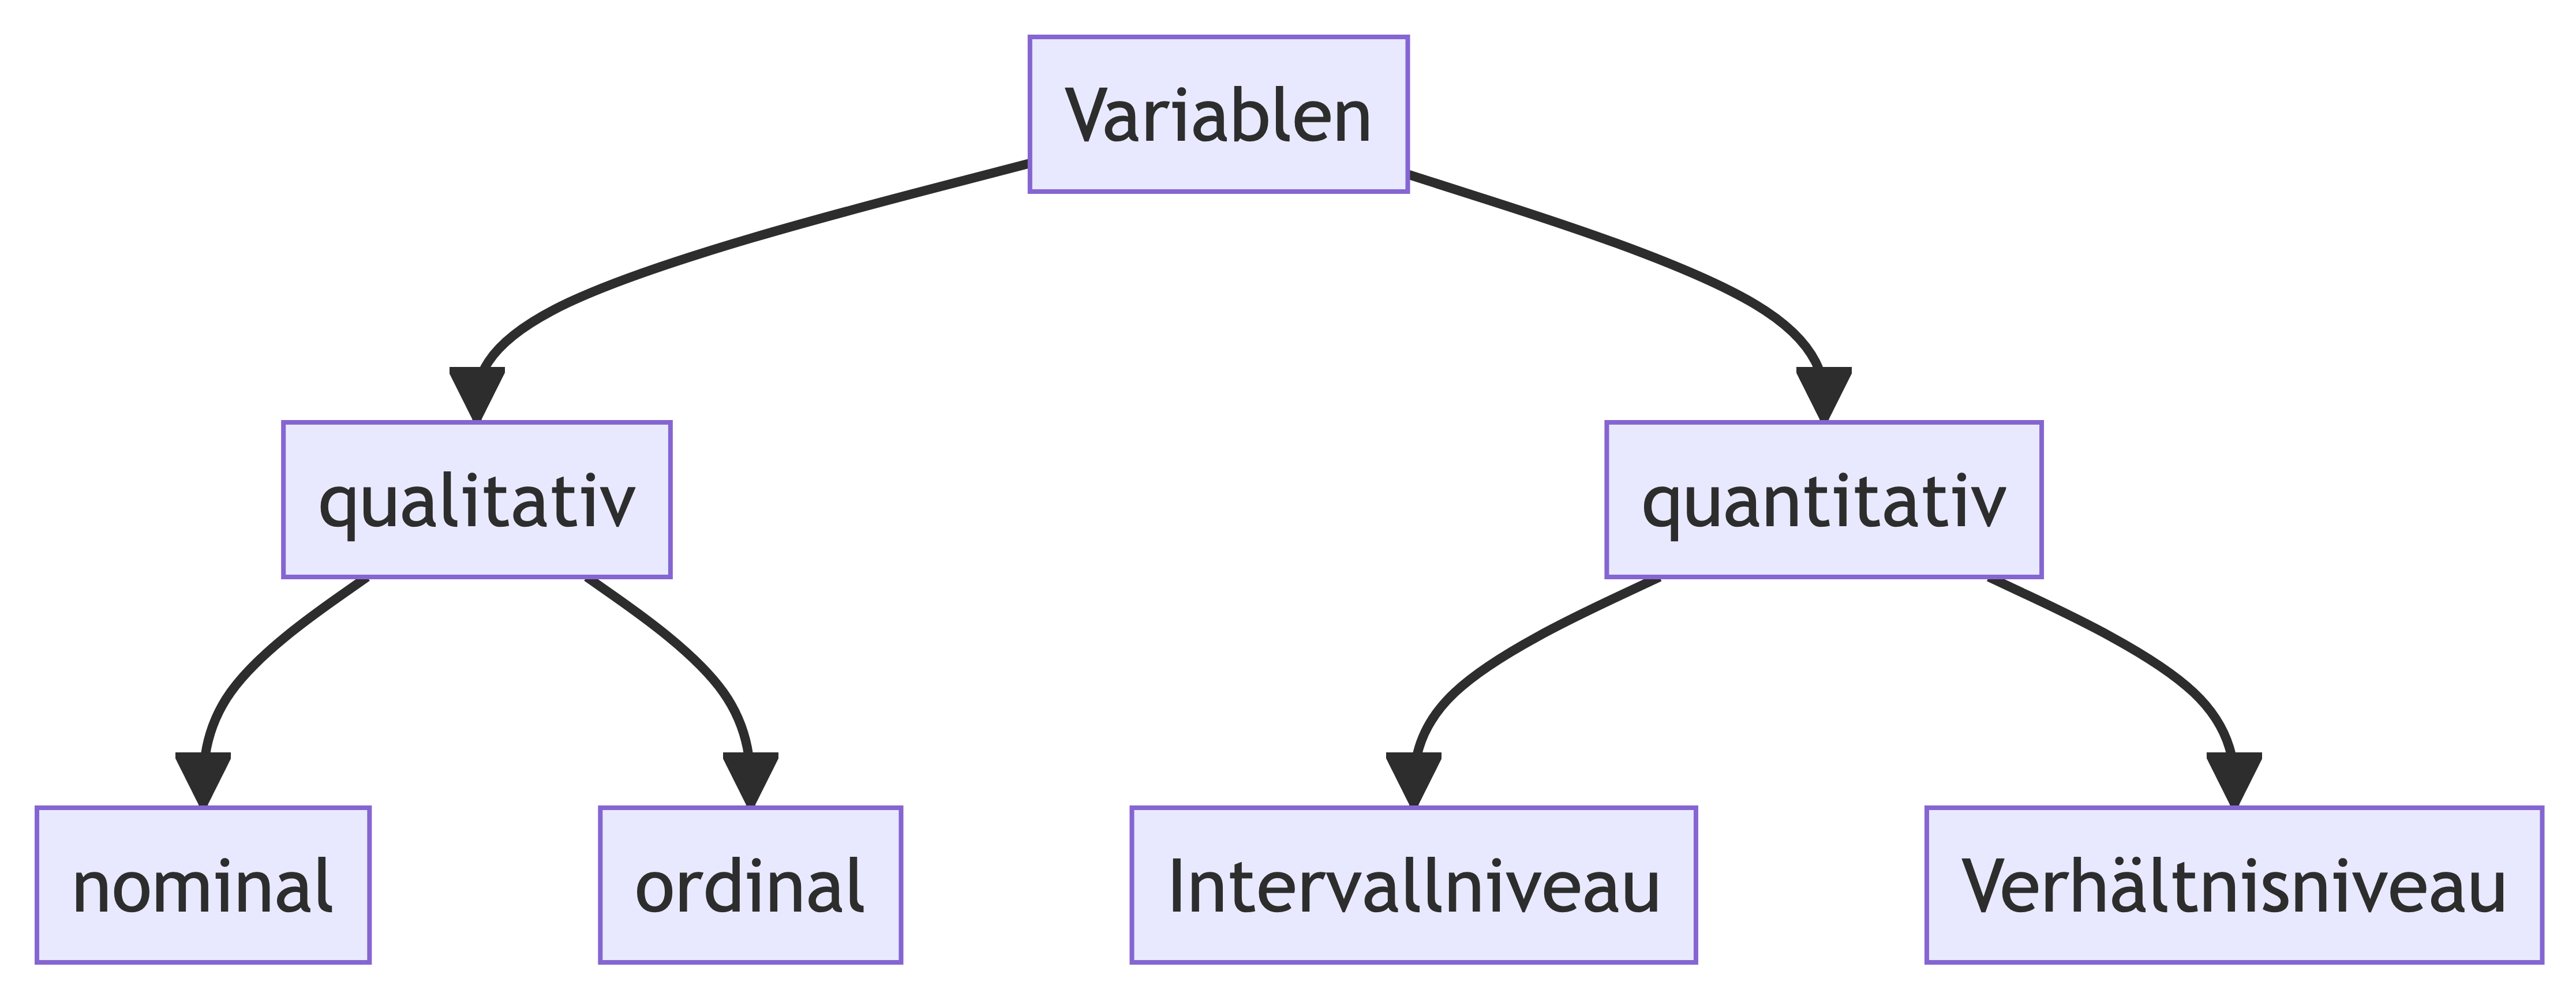
\includegraphics[width=5.82in,height=2.26in]{010-rahmen_files/figure-latex/mermaid-figure-2.png}

}

\caption{\label{fig-skalenniveau}Skalenniveaus}

\end{figure}%

\subsection{Beispiele für
Skalenniveaus}\label{beispiele-fuxfcr-skalenniveaus}

Beispiele zu den Skalenniveaus sind in Tabelle~\ref{tbl-skalen-bsps}
aufgeführt. \(\square\)

\begin{longtable}[]{@{}ll@{}}

\caption{\label{tbl-skalen-bsps}Beispiele für Skalenniveaus}

\tabularnewline

\toprule\noalign{}
Variable & Skalenniveau \\
\midrule\noalign{}
\endhead
\bottomrule\noalign{}
\endlastfoot
Haarfarbe & Nominalskala \\
Augenfarbe & Nominalskala \\
Geschlecht & Nominalskala \\
Automarke & Nominalskala \\
Partei & Nominalskala \\
Lieblingsessen & Ordinalskala \\
Medaillen beim 100-Meter-Lauf & Ordinalskala \\
Uniranking & Ordinalskala \\
IQ & Intervallskala \\
Extraversion & Intervallskala \\
Temperatur in Celcius & Intervallskala \\
Temperatur in Fahrenheit & Intervallskala \\
Temperatur in Kelvin & Verhältnisskala \\
Körpergröße & Verhältnisskala \\
Geschwindigkeit & Verhältnisskala \\
Länge & Verhältnisskala \\

\end{longtable}

Je nach dem, über welches Skalenniveau eine Variable verfügt, sind
verschiedenen Rechenoperationen erlaubt, s. {tbl-skalenniveaus-pdf}.

\begin{longtable}[]{@{}
  >{\raggedright\arraybackslash}p{(\columnwidth - 10\tabcolsep) * \real{0.2237}}
  >{\raggedright\arraybackslash}p{(\columnwidth - 10\tabcolsep) * \real{0.1579}}
  >{\raggedright\arraybackslash}p{(\columnwidth - 10\tabcolsep) * \real{0.1447}}
  >{\raggedright\arraybackslash}p{(\columnwidth - 10\tabcolsep) * \real{0.1579}}
  >{\raggedright\arraybackslash}p{(\columnwidth - 10\tabcolsep) * \real{0.1184}}
  >{\raggedright\arraybackslash}p{(\columnwidth - 10\tabcolsep) * \real{0.1974}}@{}}

\caption{\label{tbl-skalenniveaus-pdf}Erlaubte Rechenoperationen nach
Skalenniveau}

\tabularnewline

\toprule\noalign{}
\begin{minipage}[b]{\linewidth}\raggedright
Skalenniveau
\end{minipage} & \begin{minipage}[b]{\linewidth}\raggedright
Quantitativ
\end{minipage} & \begin{minipage}[b]{\linewidth}\raggedright
Gleichheit
\end{minipage} & \begin{minipage}[b]{\linewidth}\raggedright
Reihenfolge
\end{minipage} & \begin{minipage}[b]{\linewidth}\raggedright
Addition
\end{minipage} & \begin{minipage}[b]{\linewidth}\raggedright
Multiplikation
\end{minipage} \\
\midrule\noalign{}
\endhead
\bottomrule\noalign{}
\endlastfoot
Nominalniveau & nein & ja & nein & nein & nein \\
Ordinalniveau & nein & ja & ja & nein & nein \\
Intervallniveau & ja & ja & ja & ja & nein \\
Verhältnisniveau & ja & ja & ja & ja & ja \\

\end{longtable}

Was soll das bedeuten, ``Rechenoperationen''?

Schauen wir uns für jedes Skalenniveau ein ``Rechenbeispiel'' an.

\emph{Nominalskala}: Die Variable \emph{Geschlecht} ist nominalskaliert.
Das bedeutet, dass ihre Ausprägungen \emph{Frau} und \emph{Mann} z.B.
nicht (sinnvoll) addiert oder sonstwie ``verrechnet'' werden können. Man
könnte, z.B. um das Eintippen zu erleichtern, Frauen mit \texttt{1}
kodieren und Männer mit \texttt{2}. Damit darf man aber nicht rechnen!
Nicht addieren, multiplizieren \ldots{} Es macht keinen Sinn zu sagen:
``Ich habe eine Frau und einen Mann in meiner Tabelle, das ist im
Schnitt ein diverses Geschlecht, weil der Mittelwert von 1 und 2 ist
1,5!''

Die \emph{einzige} ``Rechenoperation'', die man auf der Nominalskala
machen darf, ist die Prüfung auf \emph{Gleichheit}: Mann kann
feststellen, ob ein Objekt gleich zu einem anderen ist oder
unterschiedlich. Also ob zwei Personen das gleiche Geschlecht haben oder
von unterschiedlichem Geschlecht sind. Anders ausgedrückt:

\begin{itemize}
\tightlist
\item
  FRAU \(\ne\) MANN
\item
  FRAU \(=\) FRAU
\item
  MANN \(=\) MANN
\end{itemize}

\emph{Ordinalskala}: Diese Skala entspricht einer Rangordnung. Eine
Rangordnung ist etwa die geordnete Abfolge Ihres
Leibgerichte\footnote{1. Pizza, 2. Spagetthi, 3. Schnitzel}. Etwas
``formaler'' ausgedrückt:

\begin{itemize}
\tightlist
\item
  \(\text{Pizza} \succ \text{Spagetthi} \succ \text{Schnitzel}\)
\end{itemize}

Das komische Zeichen \(\succ\) soll heißen: ``Ist auf meiner Liste von
Leibgerichten weiter oben, mag ich lieber''. Man kann aber \emph{nicht}
sagen, ``Ich mag aber Pizza um 42\% mehr als die Spagetthi und die
wieder um 73\% mehr als ein Schnitzel!''. Zumindest kann man das nicht
ohne weitere Informationen und Annahmen. Es gibt also Dinge auf der
Welt, die man leicht in eine Rangordnung bringen kann, aber die man nur
schwer in der Größe der Unterschiede bemessen kann. Das ist die
Ordinalskala.

\begin{tcolorbox}[enhanced jigsaw, colback=white, opacityback=0, arc=.35mm, titlerule=0mm, breakable, toptitle=1mm, colframe=quarto-callout-important-color-frame, title=\textcolor{quarto-callout-important-color}{\faExclamation}\hspace{0.5em}{Wichtig}, rightrule=.15mm, colbacktitle=quarto-callout-important-color!10!white, coltitle=black, leftrule=.75mm, bottomrule=.15mm, bottomtitle=1mm, opacitybacktitle=0.6, toprule=.15mm, left=2mm]

Die Ordinalskale erlaubt, Objekte zu ordnen (hinsichtlich eines
Merkmals). Die Abstände zwischen den Objekten können nicht quantifiziert
werden. \(\square\)

\end{tcolorbox}

\emph{Intervallskala}: Das ist vielleicht eine Überraschung für Sie:
Wenn es heute 10°C hat und morgen 5°C -- dann ist es heute \emph{nicht}
doppelt so warm wie morgen. Ja, 10 ist das Doppelte von 5. Aber
\emph{10° Celcius} ist \emph{nicht} doppelt so warm wie 20° Celcius.
Wenn Sie das verwundert: Das ist normal, so geht es vielen Leuten, wenn
sie das zum ersten Mal hören. Der Grund, dass es nicht erlaubt ist,
Verhältnisse (wie doppelt/halb so viel etc.) auf der Celcius-Skala zu
bilden, ist, dass der Nullpunkt der Skala, 0° C, kein echter,
physikalischer Nullpunkt ist. Bei 0° C liegt eben nicht Null
Wärmeenergie vor. Stattdessen wurde eine Wärmenergiemenge gewählt, die
für uns Menschen ganz praktisch, da augenfällig ist: der Gefrierpunkt
von Wasser. Was bei der Intervallskala erlaubt ist, ist das Addieren
(und Subtrahieren): heute 10°C, morgen 5°C, das ist ein Unterschied von
5°C. Oder: Im Schnitt waren es 7,5°C, das ist genau in der Mitte von 5
und 10°C. Abbildung~\ref{fig-intervall} versinnbildlicht die
Intervallskala.

\begin{figure}

\centering{

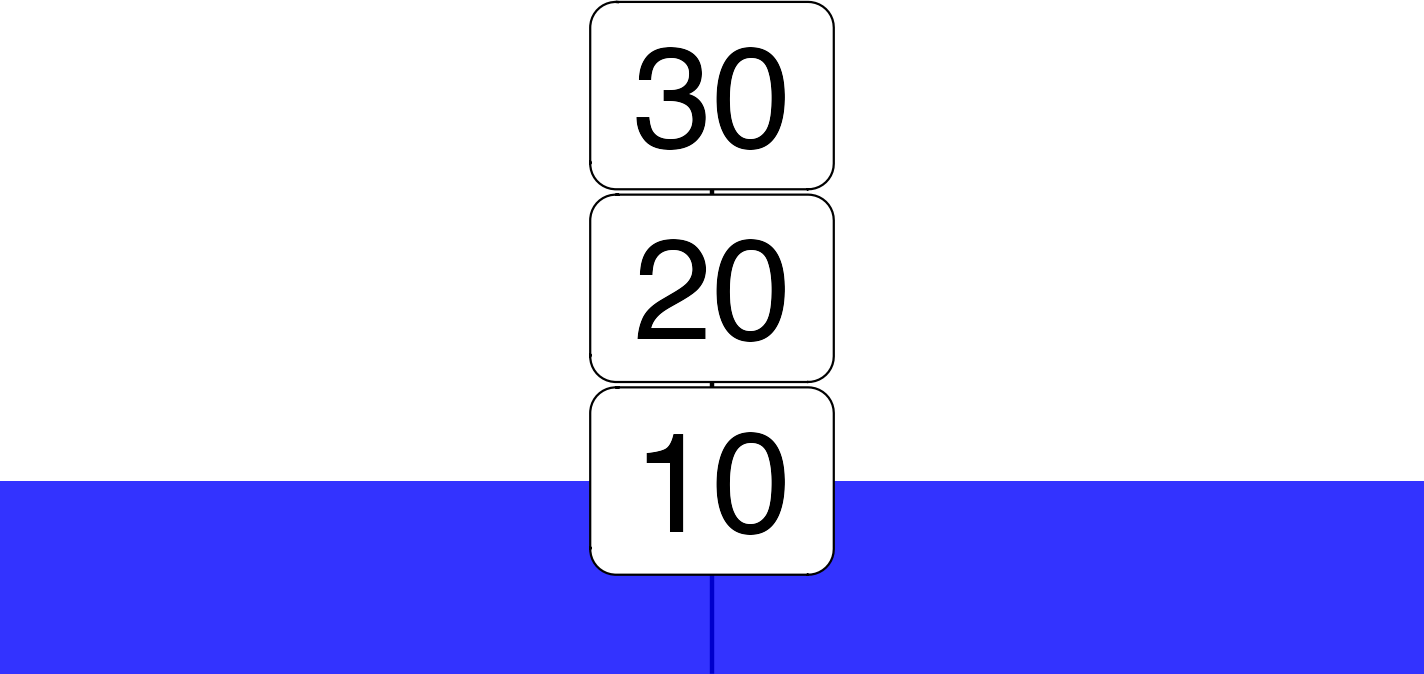
\includegraphics[width=1\textwidth,height=\textheight]{010-rahmen_files/figure-pdf/fig-intervall-1.png}

}

\caption{\label{fig-intervall}Ein Metermaß steckt im Wasser. Auf dem
Metermaß können wir die aufgedruckten Zahlen ablesen. Aber wir wissen
nicht, ob der Metermaß auf dem Boden steht. Wir wissen demnach nicht, ob
der vom Metermaß angegebene Nullpunkt der wahre Nullpunkt (Meeresboden)
ist.}

\end{figure}%

\emph{Verhältnisskala}: Eine Verhältnisskala ist das, was man sich
gemeinhin unter einer metrische Variable vorstellt: Man kann ``normal''
rechnen, alle Rechenoperationen sind erlaubt. Zuzüglich zu denen, die
auch in anderen, ``niedrigeren'' Skalenniveaus erlaubt sind, ist das das
Bilden von Verhältnissen - Multiplizieren, s.
Abbildung~\ref{fig-verhaeltnis}.

\begin{figure}

\centering{

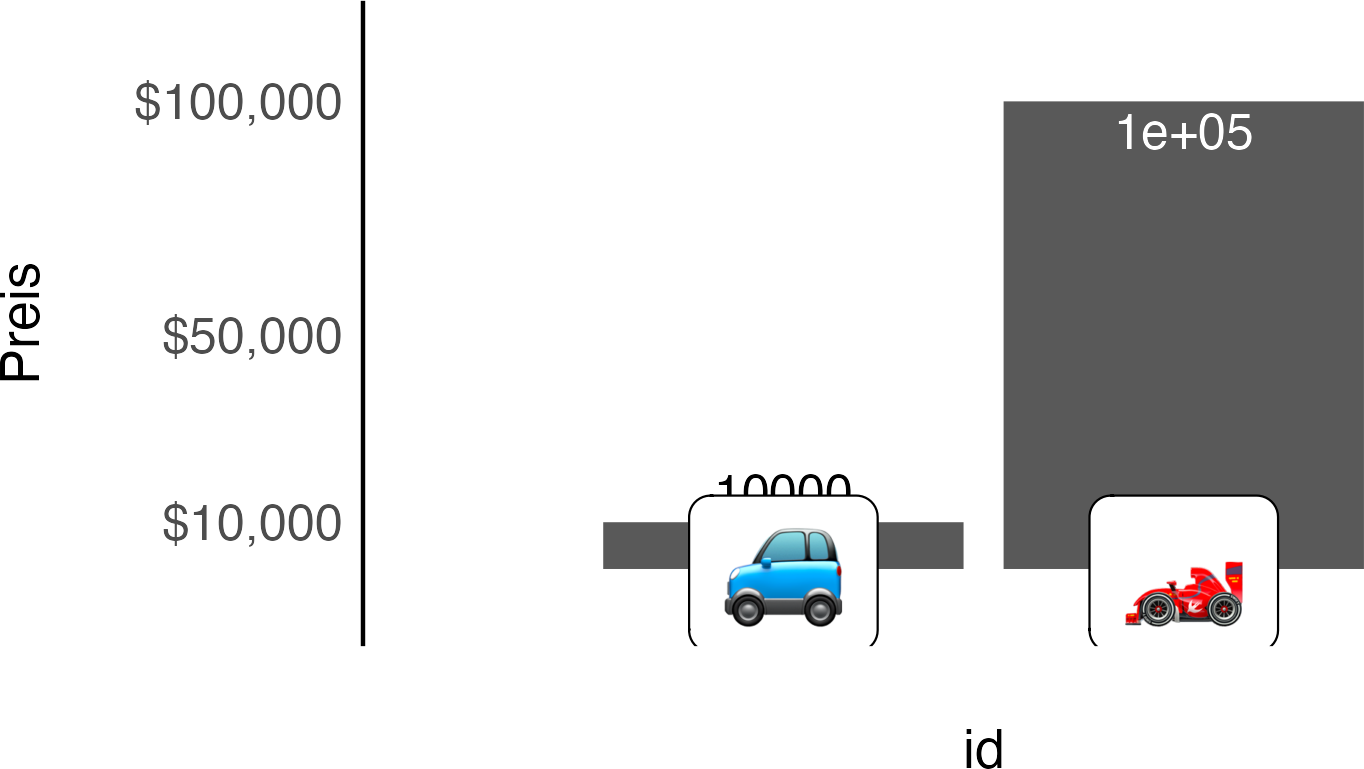
\includegraphics{010-rahmen_files/figure-pdf/fig-verhaeltnis-1.png}

}

\caption{\label{fig-verhaeltnis}Puh! Der rote Flitzer ist 10 Mal so
teuer wie die blaue Möhre. Kohlen zusammenkratzen.}

\end{figure}%

In \href{https://www.youtube.com/watch?v=_mN3kFe56ng}{diesem Video} gibt
es noch ausführlichere Erklärung zum Thema Skalenniveaus.

Außerdem können quantitative Variablen untergliedert werden in:

\begin{itemize}
\tightlist
\item
  \emph{stetige} Variablen, das sind Variablen, bei denen man zwischen
  zwei Ausprägungen immer noch eine weitere quetschen kann. So gibt es
  eine Wert für die Köpergröße zwischen 1.60\,m und 1.61\,m. Und einen
  Wert zwischen 1.601\,m und 1.602\,m, etc.
\item
  diskrete Variablen, das sind metrische Variablen, die nur bestimmte
  Ausprägungen haben, häufig sind das die natürlichen Zahlen:
  \(1,2,...\). Ein Beispiel wäre die Anzahl der Kinder in einer Familie.
\end{itemize}

\begin{tcolorbox}[enhanced jigsaw, colback=white, opacityback=0, arc=.35mm, titlerule=0mm, breakable, toptitle=1mm, colframe=quarto-callout-tip-color-frame, title=\textcolor{quarto-callout-tip-color}{\faLightbulb}\hspace{0.5em}{Tipp}, rightrule=.15mm, colbacktitle=quarto-callout-tip-color!10!white, coltitle=black, leftrule=.75mm, bottomrule=.15mm, bottomtitle=1mm, opacitybacktitle=0.6, toprule=.15mm, left=2mm]

Fragen nach Skalenniveaus gehören zu den Lieblingsprüfungsfragen in
diesem Themenbereich. Sie sind gut beraten, sich gerade mit dieser Frage
intensiver zu beschäftigen. Auch in thematisch angrenzenden Fächern wird
immer wieder die Frage nach dem Skalennvieau aufgeworfen. Das zeigt
natürlich auch die hohe Relevanz des Themas.

\end{tcolorbox}

\begin{exercise}[]\protect\hypertarget{exr-skalenniveaus}{}\label{exr-skalenniveaus}

Überlegen Sie sich für einige Variablen die Skalenniveaus und befragen
Sie dann eine:n Kommilitonen dazu. \(\square\)

\end{exercise}

\section{Modelle}\label{modelle}

Woran denken Sie beim Wort ``Modell''? Vielleicht an Spielzeugautos, s.
Abbildung~\ref{fig-matchbox}.

\begin{figure}

\centering{

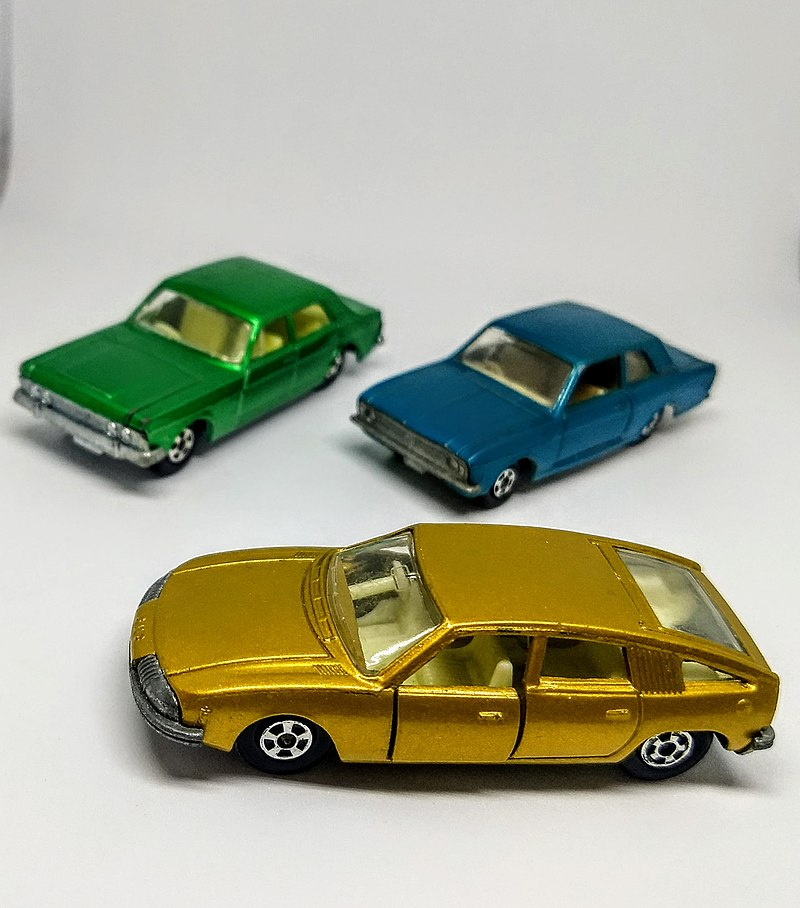
\includegraphics[width=0.25\textwidth,height=\textheight]{img/matchbox.jpg}

}

\caption{\label{fig-matchbox}Matchbox-Autos sind Modelle für Autos}

\end{figure}%

\begin{definition}[Modelle]\protect\hypertarget{def-modelle}{}\label{def-modelle}

Modelle sind ein vereinfachtes Abbild der Realität, eine
\emph{Repräsentation} (Kaplan, 2009).\(\square\)

\end{definition}

\begin{example}[Beispiele für
Modelle]\protect\hypertarget{exm-Modelle}{}\label{exm-Modelle}

Puppen sind Modelle für Babies, Landkarten für Landstriche und
\href{https://de.wikipedia.org/wiki/Bohrsches_Atommodell}{das Atommodell
von Nils Bohr} ist ein Modell für Atome.\(\square\)

\end{example}

Auch in der Statistik nutzen wir Modelle. Helfen Sie Prof.~Weiss-Ois: Er
blickt nicht durch. Gerne würde er wissen, wie viele Stunden seine
Studentis auf die Prüfung lernen. Aber mit so vielen Zahlen kann er
nicht umgehen \ldots{} Geben Sie ihm ein Modell: Sagen Sie ihm, wie lang
die Studis typischerweise lernen (sagen Sie ihm ein einfach den
Mittelwert der Lernzeiten).

\begin{figure}

\begin{minipage}{0.50\linewidth}

\section{Vorher}\label{vorher-1}

12, 8, 10, 11, 10, 9, 13, 9, 14, 9, 12, 14, 7, 9, 9, 11, 9, 4, 5, 12, 9,
6, 9, 12, 13, 9, 9, 6, 10, 8


\includegraphics[width=0.25\textwidth,height=\textheight]{img/teacher.png}

\subcaption{\label{firstcol}Oh jeh, so viele Zahlen! Ich check nix! Wie
viel lernen denn jetzt meine Studis?!}
\end{minipage}%
%
\begin{minipage}{0.50\linewidth}

\section{Nachher}\label{nachher-1}

\textbf{9.6}


\includegraphics[width=0.25\textwidth,height=\textheight]{img/teacher.png}

\subcaption{\label{secondcol}Yeah, jetzt weiß ich, wie viel die Studis
so typischerweise lernen. Viel zu wenig natürlich!}
\end{minipage}%

\end{figure}%

\href{https://www.flaticon.com/free-icons/professor}{Icon unter Flaticon
licence, Autor: iconixar}

Der Nutzen von Modellen ist, dass sie komplexe Sachverhalte vereinfachen
und damit oft überhaupt erst dem Verständnis oder einer Untersuchung
zugänglich machen: Modelle ermöglichen Verständnis. In der Datenanalyse
bzw. Statistik\footnote{die beiden Begriffe werden hier weitgehend
  synonym gebraucht} fassen Sie oft viele Daten prägnant zusammen, z.B.
zu einer einzelnen Kennzahl. Das Verrückte an Modellen ist, dass man
Informationen wegwirft, um eine (andere, hoffentlich nützlichere)
Information zu bekommen (Stigler, 2016). Weniger ist mehr?!

\section{Praxisbezug}\label{praxisbezug}

Wir leben im Datenzeitalter; Daten durchdringen alle Bereiche des
beruflichen, gesellschaftlichen und privaten Lebens. Die Datenanalyse
hat sich in den letzten Jahren massiv verändert, s.
Abbildung~\ref{fig-fo-früher-heute}.

\begin{figure}

\centering{

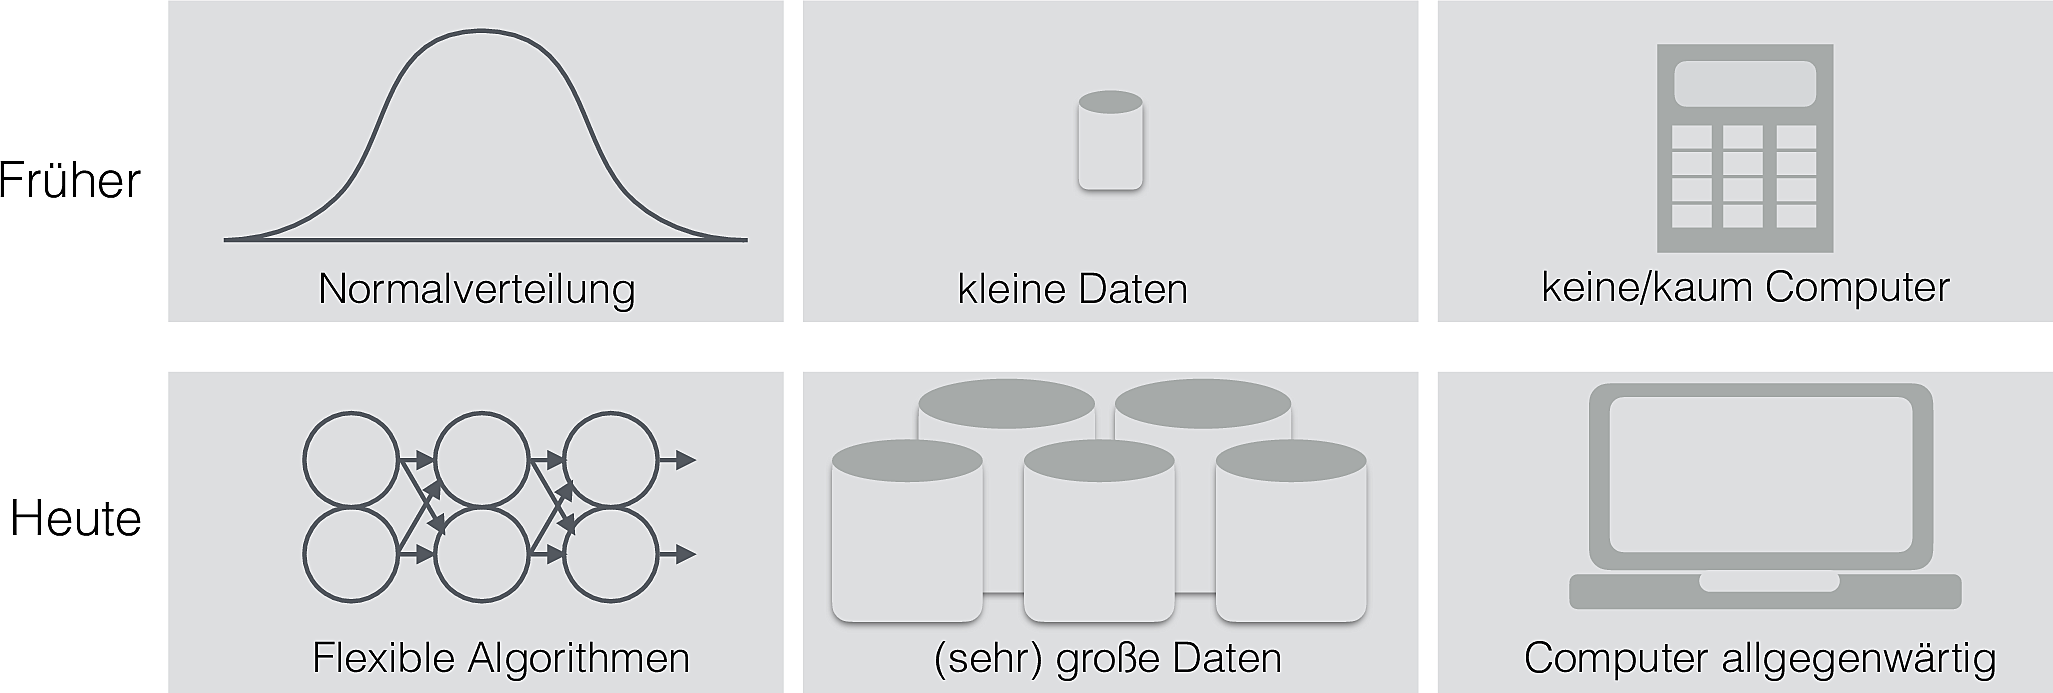
\includegraphics{img/Forschung_frueher_heute-crop.png}

}

\caption{\label{fig-fo-früher-heute}Forschung früher und heute}

\end{figure}%

Diese Entwicklung ist durchaus auch kritisch zu betrachten. Mit der
wachsenden Bedeutung von Daten wächst in gleichem Maße die Bedeutung von
Datenanalyse. Denn Daten ohne Sinn sind nutzlos. Aus diesem Grund kann
man sagen, dass Datenanalyse (und damit auch Statistik als eine
spezielle Art von Datenanalyse) zu stark nachgefragten Jobs gehören.

Laut \href{https://web.arbeitsagentur.de/entgeltatlas/beruf/129987}{dem
Entgeltatlas der Bundesagentur für Arbeit} liegt ein typisches Gehalt
von Data Scientisten bei knapp 6000 € pro Monat (in der Altersgruppe von
25 bis 54)\footnote{Abrufdatum: 1.2.23;
  \url{https://web.arbeitsagentur.de/entgeltatlas/beruf/129987}}. Laut
dem
\href{https://gehaltsreporter.de/gehaelter-von-a-bis-z/it/data-scientist/}{Gehaltsreporter}
liegt das Einstiegsgehalt dieser Berufsgruppe bei knapp 50.000€ pro
Jahr.\footnote{\url{https://gehaltsreporter.de/gehaelter-von-a-bis-z/it/data-scientist/}}

\section{Wie man mit Statistik
lügt}\label{wie-man-mit-statistik-luxfcgt}

Das \emph{File-Drawer-Problem}: Sie haben ein tolles Experiment
durchgeführt, viel Arbeit, viel Stress, endlich geschafft, puh. Von den
20 Variablen (als AV, s. Kapitel~\ref{sec-arten-variablen}), die Sie
untersucht haben, zeigt nur 1 einen interessanten Effekt, leider. 1 von
20, das hört sich nicht so toll an. Wäre es da nicht ``elegant'', die 19
Variablen ohne schönen Effekt einfach in der Schublade liegen zu lassen
bis zum Sankt-Nimmerleins-Tag? Dann könnten Sie stattdessen als Ergebnis
nur die eine Variable mit schönen Ergebnis präsentieren, ganz ohne
widersprechende Befunde.

Dieser Versuchung nicht zu erliegen, kann schwer sein. Es ist aber
gefährlich, missliebige Ergebnisse zu verschweigen: Die anderen Menschen
bekommen dann ein falsches Bild der Ergebnislage; man spricht von
\href{https://de.wikipedia.org/wiki/Publikationsbias}{Publikationsbias}.
Wer Ergebnisse verschweig, verzerrt die insgesamte Befundlage
(Rothstein, 2014).\footnote{\url{https://de.wikipedia.org/wiki/Publikationsbias}}

\section{Fazit}\label{fazit}

Die Aufgabe von Statistik ist es, durch Zusammenfassen von Daten Modelle
zu bilden, die es uns einfacher machen, schwierige Sachverhalte zu
verstehen. Zentral ist dabei, die Analyse von Variabilität der Daten.
Daten kommen in verschiedenen Varianten vor, typischerweise in
Tabellenform, möglichst im Tidy-Format.

\section{Aufgaben}\label{aufgaben}

Die Webseite \href{https://datenwerk.netlify.app}{datenwerk.netlify.app}
stellt eine Reihe von einschlägigen Übungsaufgaben bereit. Sie können
die Suchfunktion der Webseite nutzen, um die Aufgaben mit den folgenden
Namen zu suchen:

\begin{enumerate}
\def\labelenumi{\arabic{enumi}.}
\tightlist
\item
  \href{https://datenwerk.netlify.app/posts/variation01/variation01.html}{variation01}
\item
  \href{https://datenwerk.netlify.app/posts/def-statistik01/def-statistik01}{Def-Statistik01}
\item
  \href{https://datenwerk.netlify.app/posts/tidy1/tidy1.html}{tidy1}
\item
  \href{https://datenwerk.netlify.app/posts/skalenniveau1a/skalenniveau1a}{Skalenniveau1a}
\item
  \href{https://datenwerk.netlify.app/posts/ziele-statistik/ziele-statistik}{Ziele-Statistik}
\item
  \href{https://datenwerk.netlify.app/posts/variation02/variation02.html}{variation02}
\item
  \href{https://datenwerk.netlify.app/posts/skalenniveau1b/skalenniveau1b}{Skalenniveau1b}
\item
  \href{https://datenwerk.netlify.app/posts/tidydata1/tidydata1.html}{tidydata1}
\end{enumerate}

\section{Vertiefung}\label{vertiefung}

\subsection{Excel für Könner}\label{excel-fuxfcr-kuxf6nner}

In vielen Organisationen werden Exceltabellen für bestimmte Zwecke der
Datenverarbeitung verwendet. Excel\footnote{und ähnliche Programme} hat
bestimmte Stärken und Vorteile, aber auch gewisse Nachteile und
Schwäche; das liegt z.T. daran, dass Excel für bestimmte Aufgaben besser
und für andere weniger gut geeignet ist. Wenn man mit Excel arbeitet,
wiederholen sich erfahrungsgemäß immer wieder die gleichen Fehler bzw.
suboptimalen Vorgehensweise zum Aufbau einer Exceltabelle.

\href{https://www.tandfonline.com/doi/full/10.1080/00031305.2017.1375989}{Dieser
Artikel} von Broman \& Woo (2018) zeigt anhand einiger praktischer
Tipps, wie man Exceltabellen so aufbaut, dass Fehler minimiert werden.

\begin{exercise}[Fassen Sie den Artikel von Broman \& Woo (2018)
zusammen]\protect\hypertarget{exr-xls-paper}{}\label{exr-xls-paper}

Die Lehrkraft teilt Sie dazu in Gruppen ein und weist jeder Gruppe einen
Abschnitt des Artikels zu. Fassen Sie das \emph{Wesentliche} (und nur
das Wesentliche) an einem geeigneten Ort zusammen (z.B. auf einem
Miro-Board). \(\square\)

\end{exercise}

\subsection{Sind wir süchtig nach dem
Handy?}\label{sind-wir-suxfcchtig-nach-dem-handy}

Sind Sie süchtig nach Ihrem Handy? Lassen Sie uns eine kleine Studie
dazu live im Hörsaal durchführen. Füllen Sie
\href{https://forms.gle/PP8yb6Ubqq3JU78F9}{diese Umfrage} zum Thema
Smartphonse-Sucht aus (anonym und kein Muss). Wir werden die Daten
später zusammen aus. \(\square\)

\subsection{Datenprofi plaudert aus dem
Nähkästchen}\label{datenprofi-plaudert-aus-dem-nuxe4hkuxe4stchen}

Inspiration von einer Praktikerin der Datenanalyse: Caitlin Hudon verrät
\href{https://www.youtube.com/watch?v=O5lP6XcopdQ&list=PL9HYL-VRX0oQchs7dqFICoxMgnvFO10tC&index=15&t=1s}{in
diesem Video}, welche Fehler Sie sie in in den acht Jahren ihrer
Berufserfahrung gemacht hat und was sie daraus gelernt hat.

\url{https://www.youtube.com/watch?v=O5lP6XcopdQ&list=PL9HYL-VRX0oQchs7dqFICoxMgnvFO10tC&index=15&t=1s}

\section{Literaturhinweise}\label{literaturhinweise}

Einen Einblick in die Fundamente statistischer Analyse bietet Stigler
(2016). Çetinkaya-Rundel \& Hardin (2021), stellen grundlegende Konzepte
der Analyse von Daten im Kapitel 1, ``Hello data'', vor. Downey (2023)
illustriert statistische Überraschungsmoment auf unterhaltsame, und vor
allem: sofataugliche Art.

\section{Literatur}\label{literatur-1}

\chapter{Daten einlesen}\label{daten-einlesen}

\section{Lernsteuerung}\label{lernsteuerung-1}

\subsection{Standort im Lernpfad}\label{standort-im-lernpfad-1}

Abb. Abbildung~\ref{fig-ueberblick} den Standort dieses Kapitels im
Lernpfad und gibt damit einen Überblick über das Thema dieses Kapitels
im Kontext aller Kapitel.

\subsection{Lernziele}\label{lernziele-2}

\begin{itemize}
\tightlist
\item
  Sie können R und RStudio starten.
\item
  Sie können R-Pakete installieren und starten.
\item
  Sie können Variablen in R zuweisen und auslesen.
\item
  Sie können Daten in R importieren.
\item
  Sie können den Begriff \emph{Reproduzierbarkeit} definieren.
\end{itemize}

\subsection{Überblick}\label{uxfcberblick-1}

Abbildung~\ref{fig-ueberblick} zeigt Ihnen, wo auf unserer Reise durch
die Datenanalyse sich dieses Kapitels verorten lässt.

Abbildung~\ref{fig-roller} zeigt den typischen Lernverlauf in
Zusammenhang mit Datenanalyse (und R) an: Es gibt Höhen und Tiefen. Die
wechseln sich ab. Das ist ganz normal!

\begin{figure}

\centering{

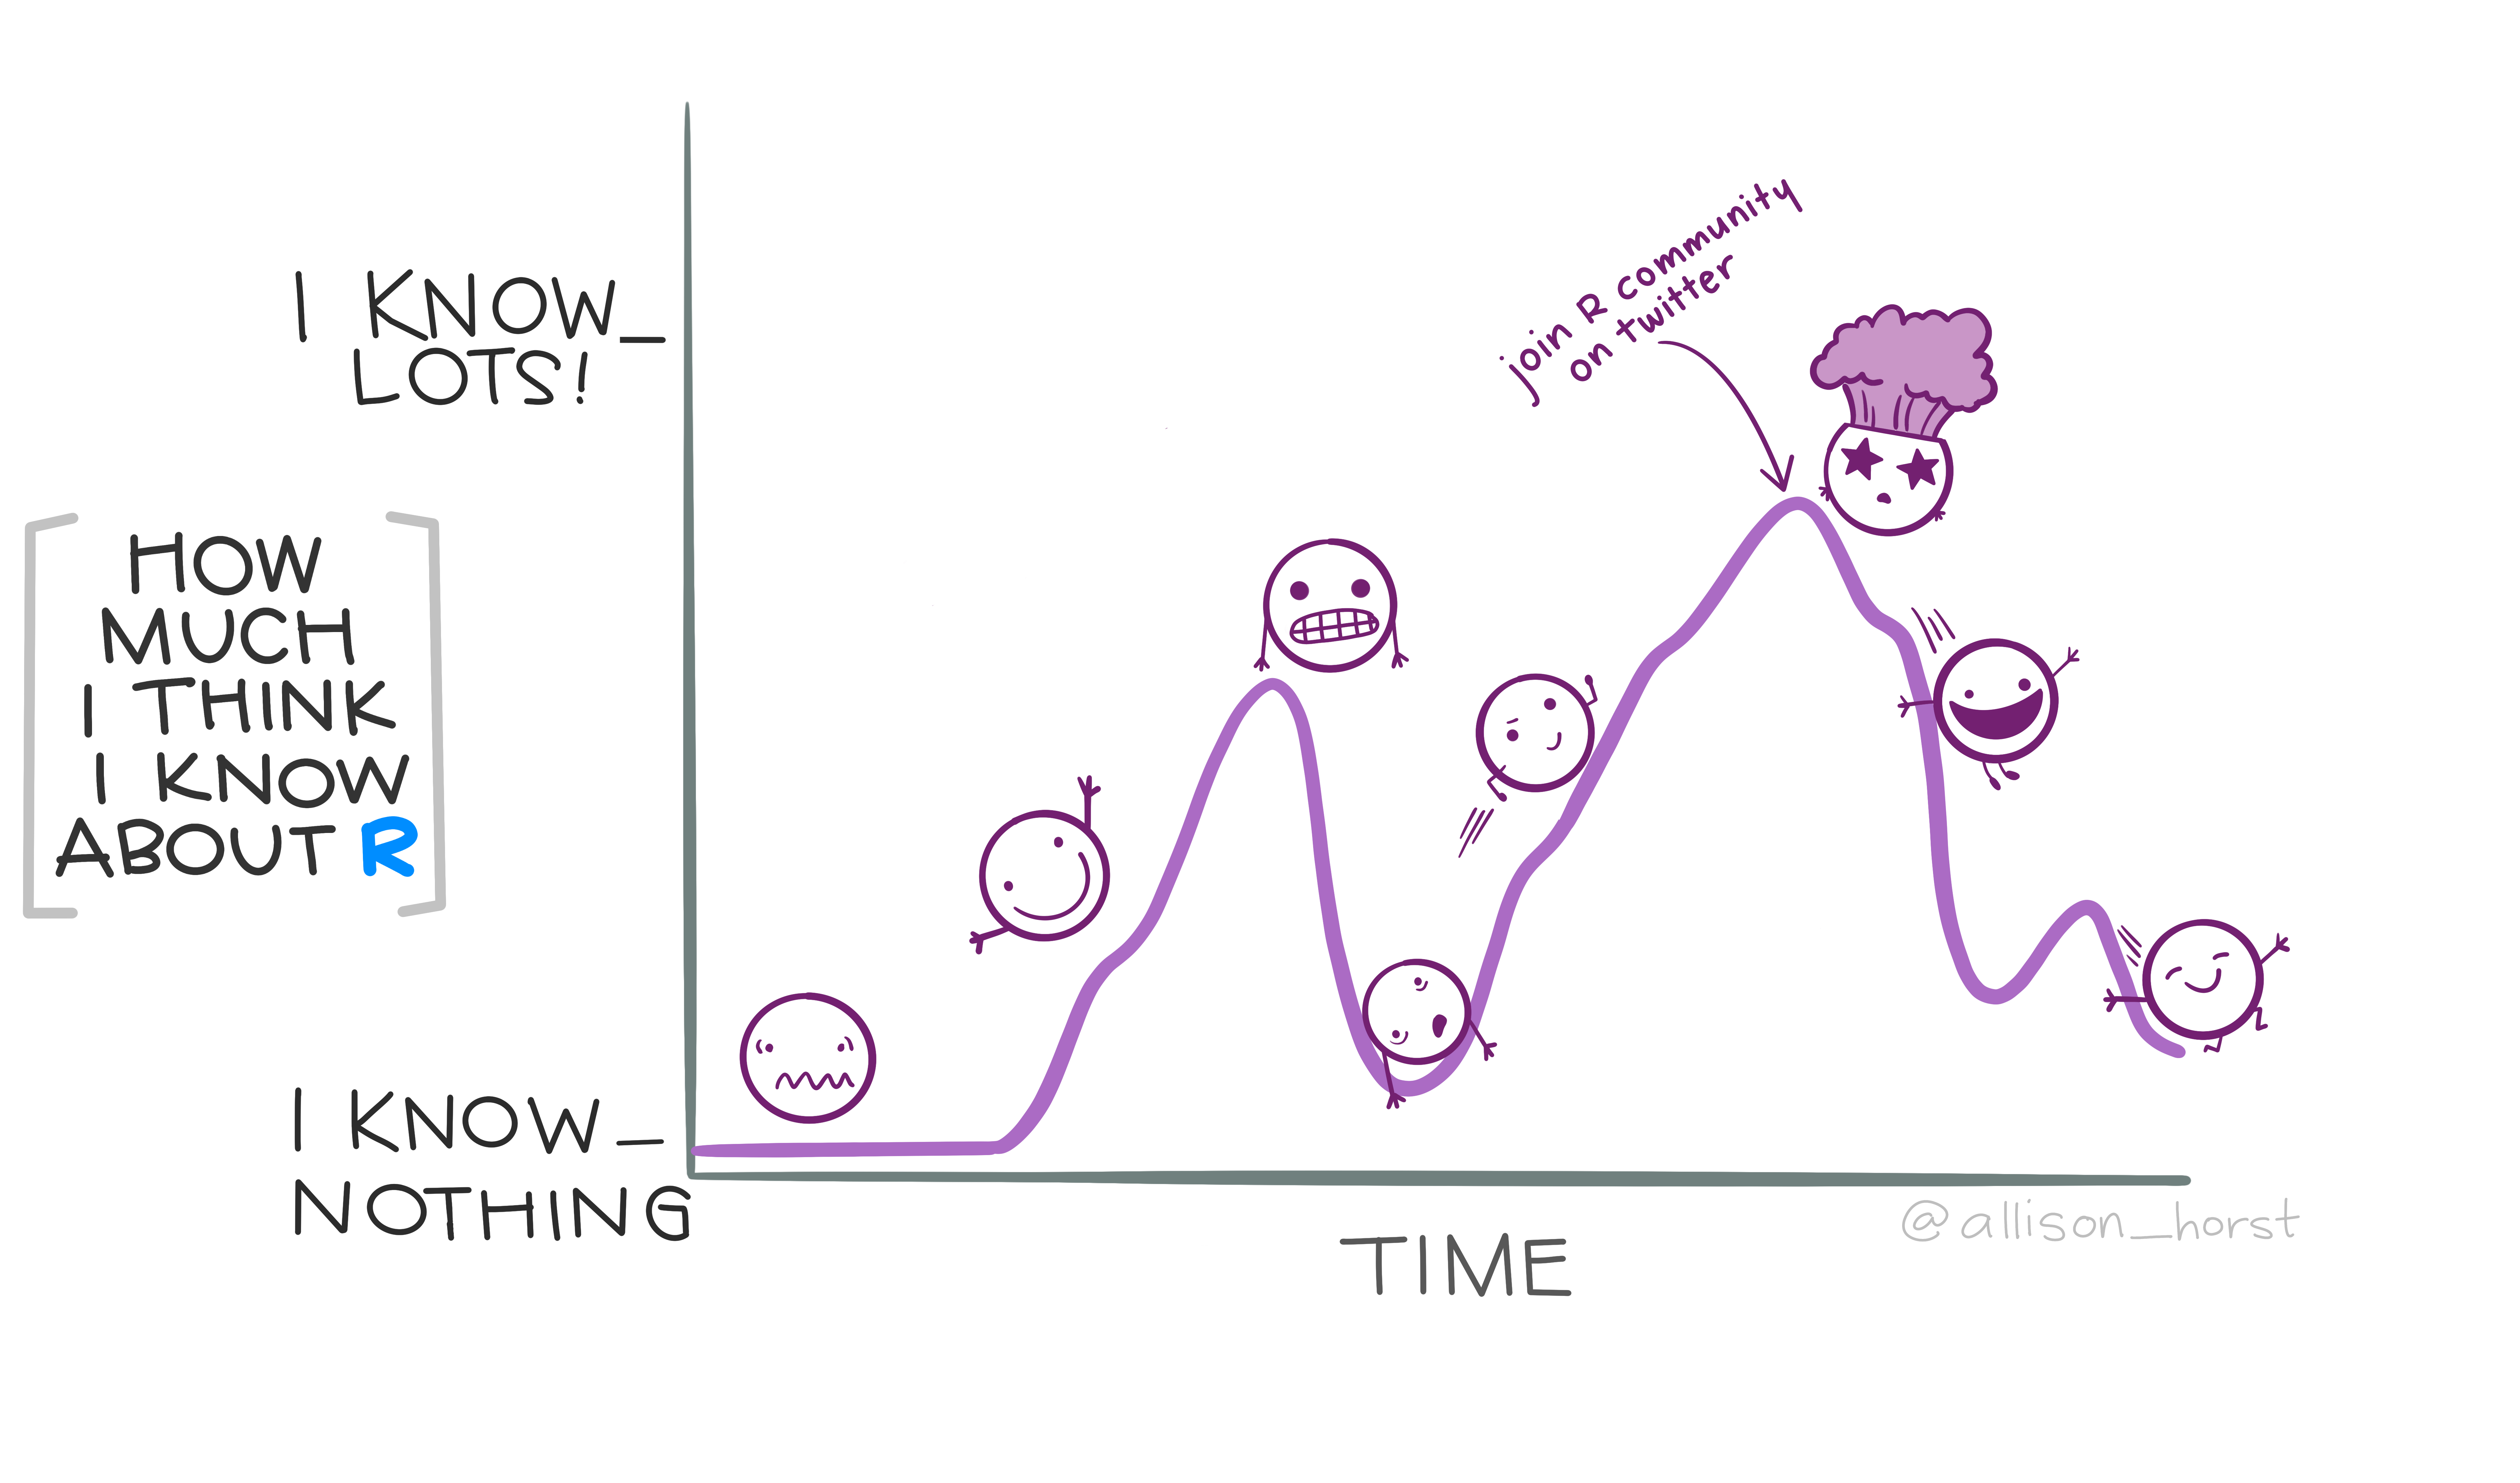
\includegraphics[width=0.8\textwidth,height=\textheight]{img/r_rollercoaster.png}

}

\caption{\label{fig-roller}Life is a roller-coaster. You just have to
ride it. Image credit: Allison Horst;
\url{https://github.com/allisonhorst/stats-illustrations}, CC-BY}

\end{figure}%

\subsection{Ab diesem Kapitel benötigen Sie
R}\label{ab-diesem-kapitel-benuxf6tigen-sie-r}

Bitte stellen Sie sicher, dass Sie R rechtzeitig einsatzbereit haben.
Weiter unten in diesem Kapitel finden Sie Installationshinweise
(Kapitel~\ref{sec-install-r}). Falls Sie dieses Kapitel zum ersten Mal
bzw. sich noch nicht mir R auskennen, werden Sie vielleicht einigen
Inhalten begegnen, die Sie noch nicht gleich verstehen. Keine Sorge, das
ist normal. Mit etwas Übung wird Ihnen bald alles schnell von der Hand
ghen.

\subsection{Begleitvideos}\label{begleitvideos}

Schauen Sie sich malden YouTube-Kanal
\texttt{@sebastiansauerstatistics}\footnote{\url{https://www.youtube.com/@sebastiansauerstatistics}}
an und dort die Playlist ``R''\footnote{\url{https://www.youtube.com/playlist?list=PLRR4REmBgpIEaIyeNBgNGPgmhQJ_T1y8_}}.
Dort finden Sie einige Videos zum Thema R.

\section{Errrstkontakt}\label{errrstkontakt}

\subsection{Warum R?}\label{warum-r}

Gründe, die für den Einsatz von R sprechen:

\begin{enumerate}
\def\labelenumi{\arabic{enumi}.}
\item
  🆓 R ist kostenlos, andere Softwarepakete für Datenanalyse sind teuer.
  💸
\item
  📖 R und R-Befehle sind quelloffen, d.h. man kann sich die
  zugrundeliegenden Computerbefehle anschauen. Jede/r kann prüfen, ob R
  vernünftig arbeitet. Jede/r kann beitragen.
\item
  🆕 R hat die neuesten Methoden.
\item
  🫂 R hat eine große Community.
\item
  🪡 R ist maßgeschneidert für Datenanalyse.
\end{enumerate}

Allerdings gibt es auch abweichende Meinungen, s.
Abbildung~\ref{fig-bill-excel}.

\begin{figure}

\centering{


\includegraphics[width=0.5\textwidth,height=\textheight]{img/bill-gates-excel.jpg}

}

\caption{\label{fig-bill-excel}Manche finden Excel cooler als R, nicht
wahr, Bill Gates?}

\end{figure}%

\subsection{R und Reproduzierbarkeit}\label{r-und-reproduzierbarkeit}

\begin{definition}[Reproduzierbarkeit]\protect\hypertarget{def-repro}{}\label{def-repro}

Ein (wissenschaftlicher) Befunde ist reproduzierbar, wenn andere
Analystis mit dem gleichen experimentellen Setup zum gleichen Ergebnis
(wie in der ursprünglichen Analyse) kommen (Plesser, 2018). \(\square\)

\end{definition}

Definition~\ref{def-repro} ist, etwas überspitzt, in
Abbildung~\ref{fig-repro} wiedergegeben.

\begin{figure}

\centering{


\includegraphics[width=0.5\textwidth,height=\textheight]{img/repro-star-struck.png}

}

\caption{\label{fig-repro}Daten + Syntax + genaue Beschreibung der
Messungen = reproduzierbar}

\end{figure}%

\begin{example}[Aus der Forschung: Reproduzierbarkeit in der
Psychologie]\protect\hypertarget{exm-repro}{}\label{exm-repro}

~

\begin{quote}
🧑‍🎓 Wie ist es um unsere Wissenschaft, Psychologie, bestellt? Haben die
Befunde Hand und Fuß?
\end{quote}

Obels et al. (2020) haben die Reproduzierbarkeit in psychologischen
Studien untersucht. Sie berichten folgendes Ergebnis

\begin{quote}
We examined data and code sharing for Registered Reports published in
the psychological literature from 2014 to 2018 and attempted to
independently computationally reproduce the main results in each
article. Of the 62 articles that met our inclusion criteria, 41 had data
available, and 37 had analysis scripts available. Both data and code for
36 of the articles were shared. We could run the scripts for 31
analyses, and we reproduced the main results for 21 articles.
\(\square\)
\end{quote}

\end{example}

\subsection{R \& RStudio}\label{r-rstudio}

Wenn wir sagen, ``wir arbeiten mit R'', dann heißt das in unserem Fall
``wir arbeiten mit R und mit RStudio''.


\includegraphics[width=0.2\textwidth,height=\textheight]{img/R-logo.png}

💖


\includegraphics[width=0.4\textwidth,height=\textheight]{img/rlogo.png}

Ismay \& Kim (2020) zeigen eine schöne Analogie, was der Unterschied von
\emph{R} und \emph{RStudio} ist, s.
Abbildung~\ref{fig-r-rstudio}.\footnote{Streng genommen ist RStudio für
  die Datenanalyse irrelevant, aber RStudio ist praktisch, Sie werden es
  nicht missen wollen.}

\begin{figure}

\centering{

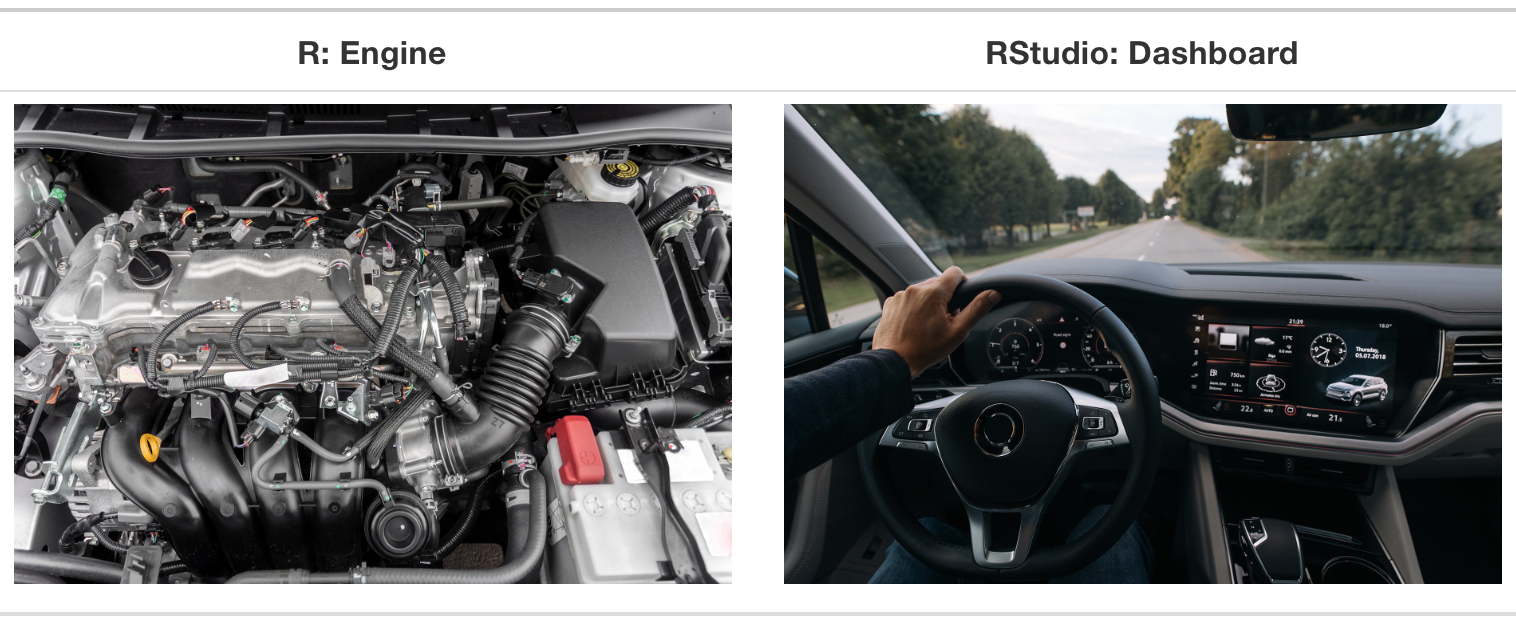
\includegraphics[width=5.05in,height=\textheight]{img/r_vs_rstudio_1.png}

}

\caption{\label{fig-r-rstudio}R vs.~RStudio: R macht die Arbeit, RStudio
ist für Komfort und Übersicht}

\end{figure}%

Kurz gesagt: Das eigentlich Arbeiten besorgt R. Für den Komfort und die
Schönheit ist RStudio zuständig. Auch eine Art von Arbeitsteilung!

\begin{tcolorbox}[enhanced jigsaw, colback=white, opacityback=0, arc=.35mm, titlerule=0mm, breakable, toptitle=1mm, colframe=quarto-callout-note-color-frame, title=\textcolor{quarto-callout-note-color}{\faInfo}\hspace{0.5em}{Hinweis}, rightrule=.15mm, colbacktitle=quarto-callout-note-color!10!white, coltitle=black, leftrule=.75mm, bottomrule=.15mm, bottomtitle=1mm, opacitybacktitle=0.6, toprule=.15mm, left=2mm]

\begin{itemize}
\tightlist
\item
  R: 🏋️‍♀️
\item
  RStudio: 💅 \(\square\)
\end{itemize}

\end{tcolorbox}

Hier sehen Sie einen Screenshot von der Oberfläche von RStudio, s.
Abbildung~\ref{fig-rstudio}.

\begin{figure}

\centering{

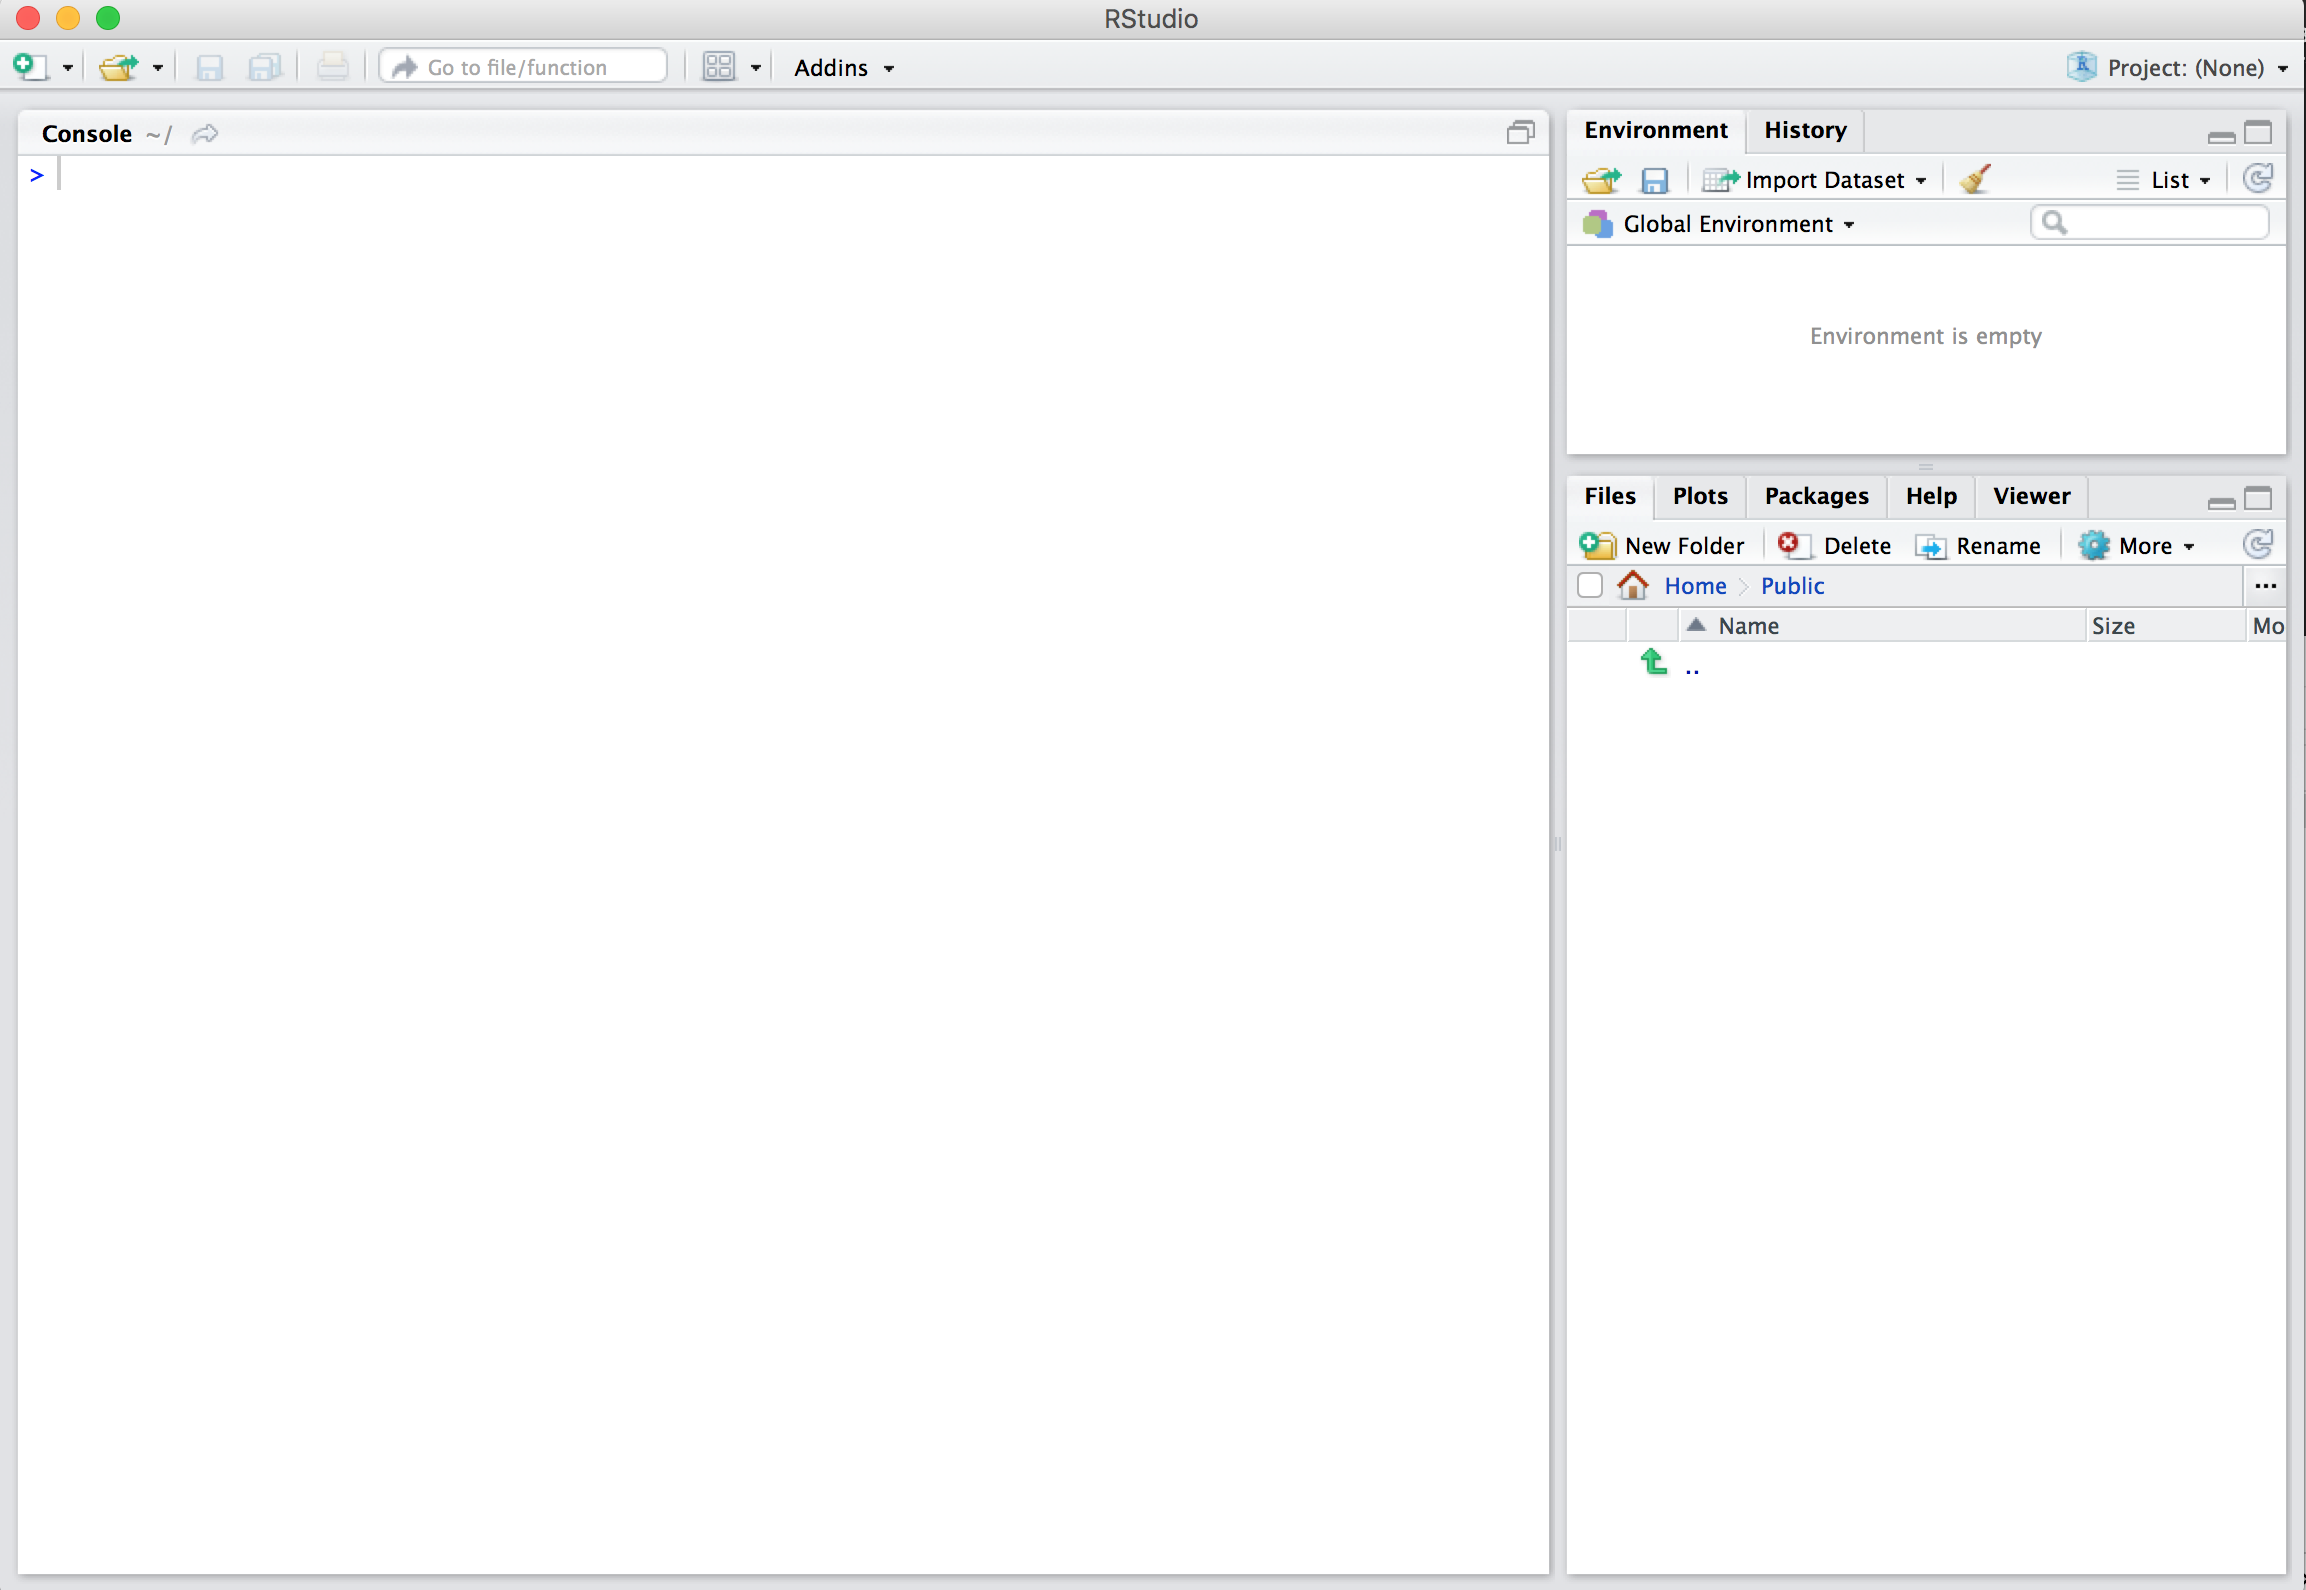
\includegraphics{img/rstudio.png}

}

\caption{\label{fig-rstudio}So sieht RStudio aus}

\end{figure}%

\section{Installation von R und RStudio}\label{sec-install-r}

\subsection{Installation von R}\label{installation-von-r}

R ist ein Softwarepaket für statistische Berechnungen\footnote{Mehr
  Infos finden sich hier:
  \url{https://de.wikipedia.org/wiki/R_\%28Programmiersprache\%29}}.
Laden Sie es für Ihr Betriebssytem herunter:

\begin{itemize}
\tightlist
\item
  \href{https://cloud.r-project.org/bin/windows/base/}{Windows}
\item
  \href{https://cloud.r-project.org/bin/macosx/}{MacOS}
\item
  \href{https://cloud.r-project.org/bin/linux/}{Linux}
\end{itemize}

Mehr Infos zu R finden Sie unter
\url{https://cloud.r-project.org/}.\footnote{Wenn Sie gefragt werden,
  dass Sie einen ``Mirror'' auswählen sollen, heißt das, Sie sollen
  einen Computer (Server) wählen, von dem Sie R herunterladen. Der
  sollte möglichst nicht zu weit weg stehen, dann spart es vielleicht
  etwas Zeit und Bandbreite.}

Wenn Sie die Installationsdatei heruntergeladen haben, öffnen Sie diese
Datei (Doppelklick) und Sie werden durch die Installation
geführt.\footnote{Sie benötigen Admin-Rechte auf Ihrem Computer.}

\subsection{Installation von RStudio}\label{installation-von-rstudio}

RStudio ist eine \emph{graphische Benutzeroberfläche} (graphical user
interface, GUI) für R, plus ein paar Goodies\footnote{in Form einer
  \emph{intergrierten Entwicklungsumgebung} (integrated development
  environment, IDE:
  \url{https://en.wikipedia.org/wiki/Integrated_development_environment}))}.

Laden Sie zunächst die \emph{Desktop-Version} von RStudio herunter für
Ihr Betriebssystem (Windows, MacOS, Linux) vom Anbieter (Posit)
herunter. \footnote{\url{https://posit.co/download/rstudio-desktop/}}.

Wenn Sie die Installationsdatei heruntergeladen haben, öffnen Sie diese
Datei (Doppelklick) und Sie werden durch die Installation
geführt.\footnote{Sie benötigen Admin-Rechte auf Ihrem Computer.}

\subsection{RStudio Cloud}\label{rstudio-cloud}

\subsubsection{RStudio Cloud als Alternative zu
RStudio}\label{rstudio-cloud-als-alternative-zu-rstudio}

RStudio Cloud\footnote{\url{https://rstudio.cloud/}; neuerdings auch
  ``Posit Cloud'' genannt} ist ein Webdienst von Posit/RStudio (zum Teil
kostenlos), also \emph{RStudio online}: Man kann damit online mit R
arbeiten. Die Oberfläche ist praktisch identisch zur Desktop-Version, s.
Abbildung~\ref{fig-rstudio-cloud}. Sie können es als Alternative zur
Installation von RStudio auf Ihrem Computer verwenden. Ein Vorteil von
RStudio Cloud ist, dass man als Nutzer \emph{nichts installieren} muss
und dass es \emph{auch auf Tablets} läuft (im Gegensatz zur
Desktop-Version von RStudio). Ein Nachteil ist, dass es etwas langsamer
ist und nur für ein gewisses Zeitvolumen kostenlos. Sie müssen sich ein
Konto anlegen, um den Dienst nutzen zu können.

\begin{figure}

\centering{

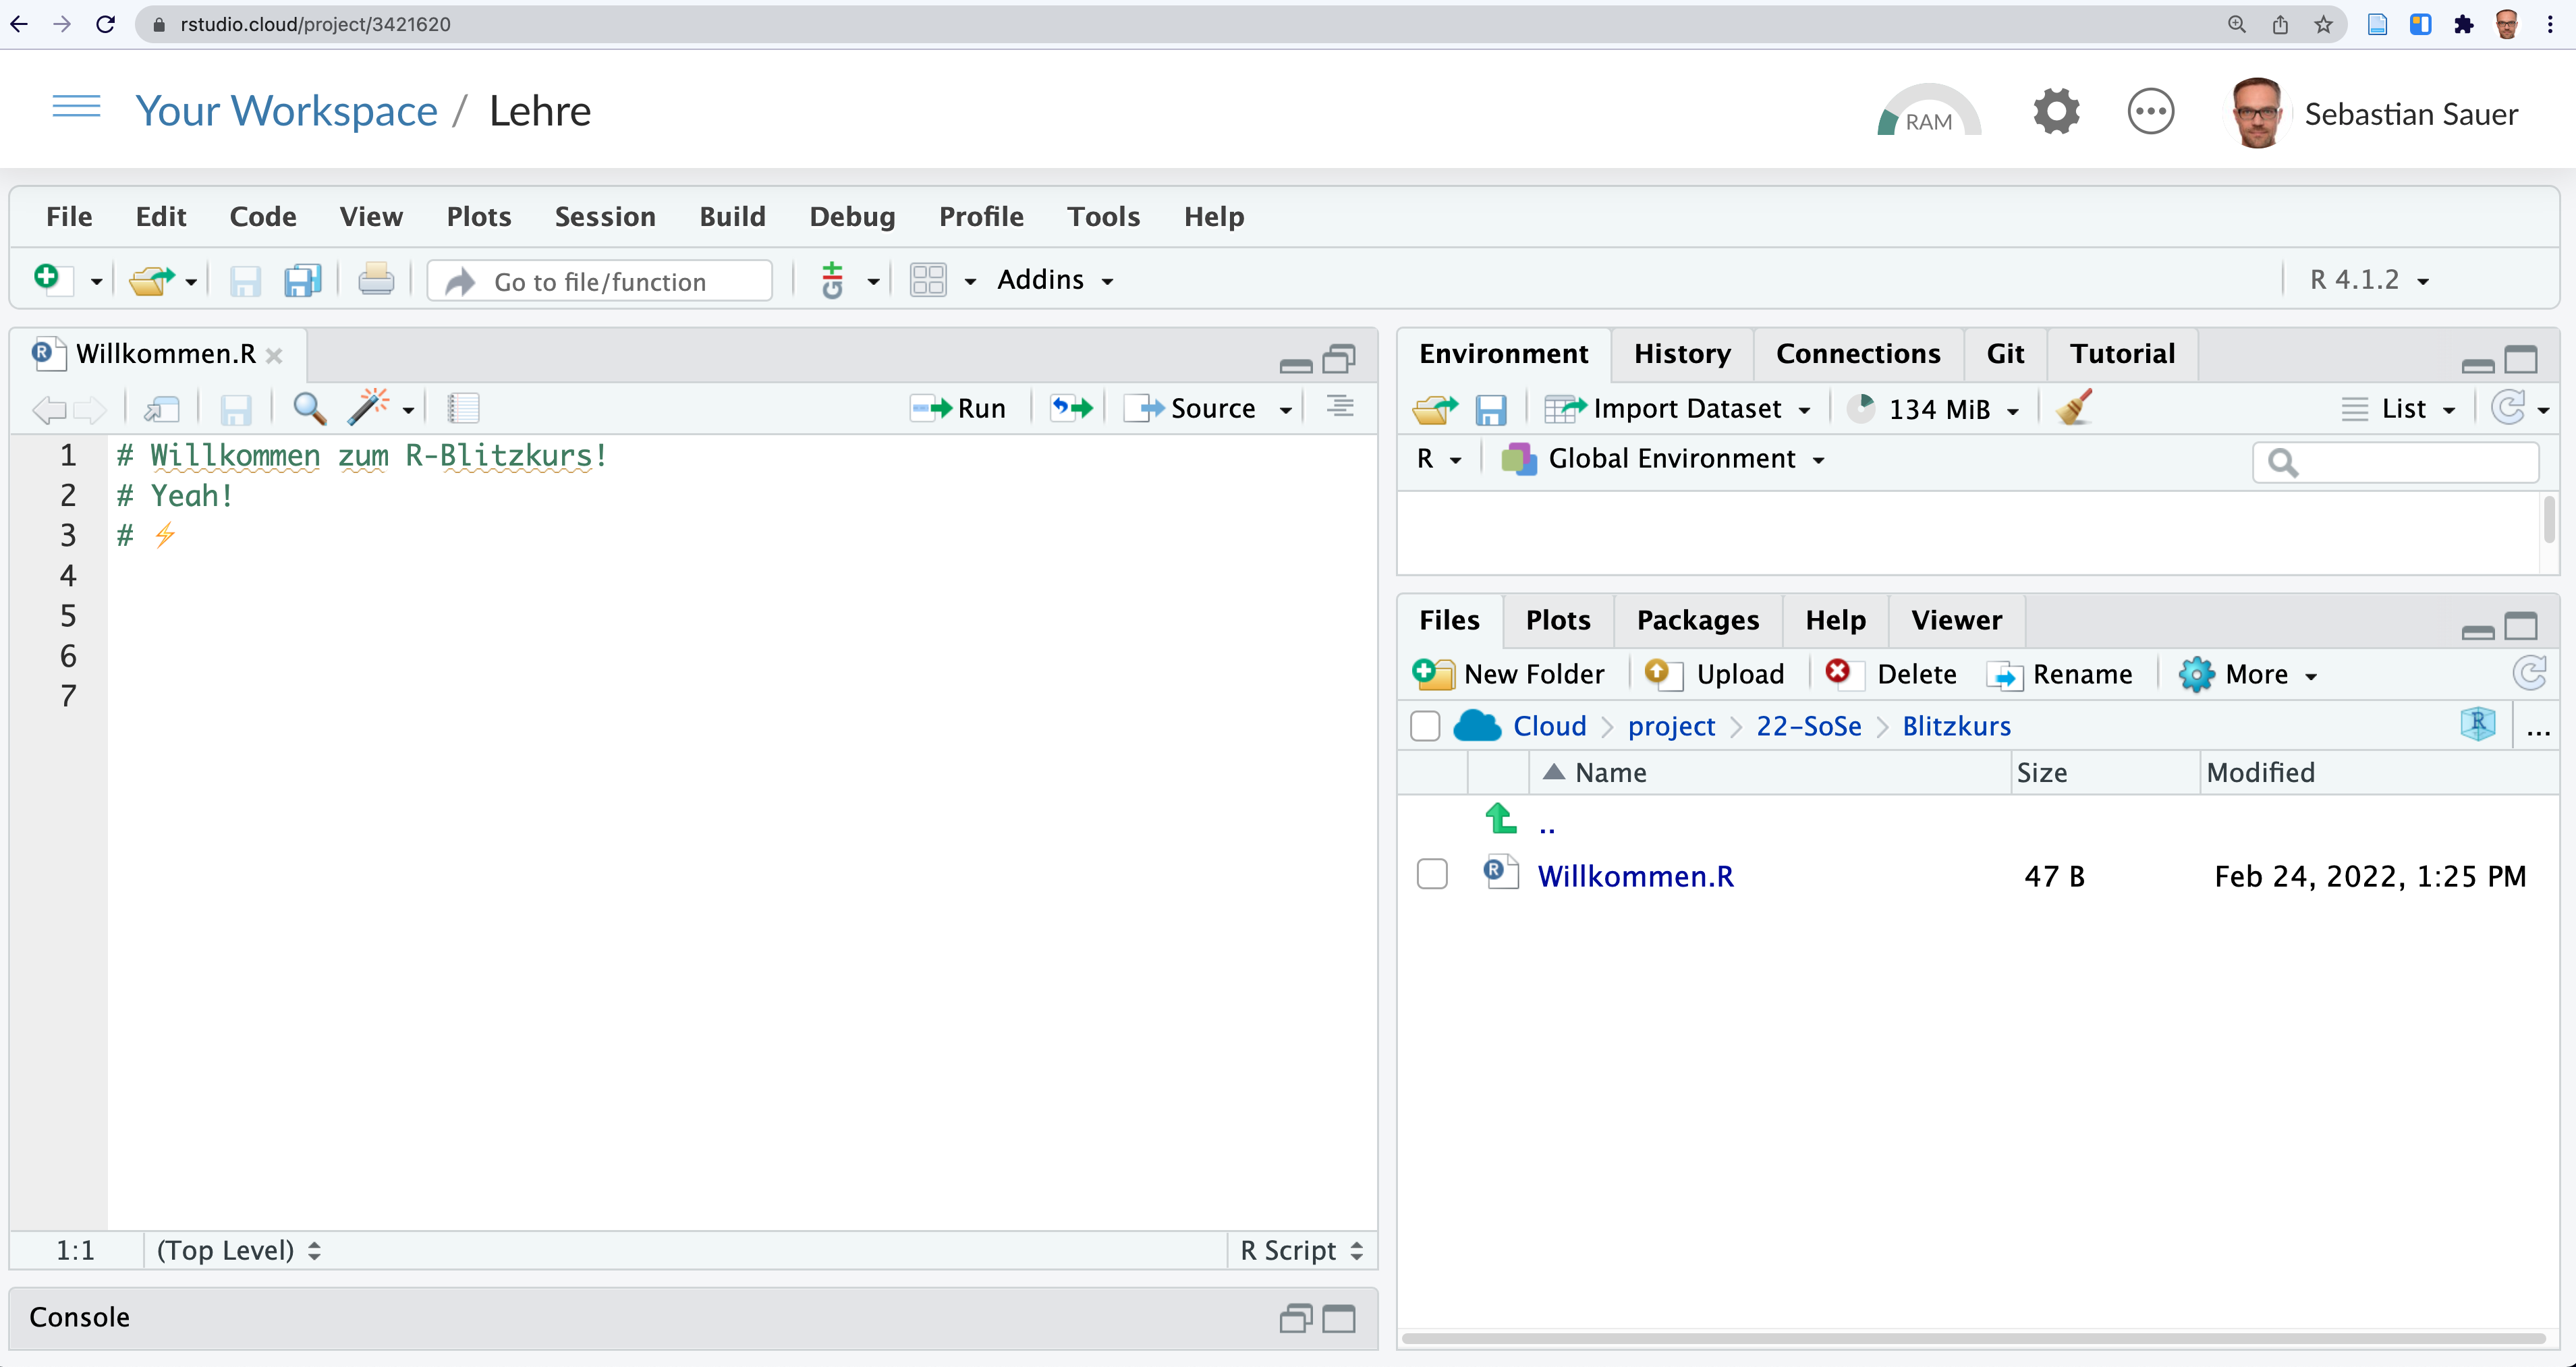
\includegraphics{img/rstudio-cloud.png}

}

\caption{\label{fig-rstudio-cloud}So sieht RStudio Cloud aus. Genau wie
RStudio Desktop}

\end{figure}%

\subsubsection{Vertiefung}\label{vertiefung-1}

Wenn Ihr Dozent Ihnen einen Projektordner bzw. einen Link dazu
bereitstellt, ist das komfortabel, da der Dozent dann schon Pakete
installieren, Daten bereitstellen und andere Nettigkeit vorbereiten kann
für Sie. Allerdings müssen Sie den Projektordner in Ihrem Konto
abspeichern, wenn Sie etwas speichern möchten, da Sie vermutlich keine
Schreibrechte im Projektordner Ihres Dozenten haben. Klicken Sie dazu
auf ``Save a permanent copy'', s. Abbildung~\ref{fig-perm-copy}.

\begin{figure}

\centering{


\includegraphics{img/rstudio-save-a-permanent-copy.png}

}

\caption{\label{fig-perm-copy}Einen Projektordner im eigenen Konto
abspeichern, um Schreibrechte zu haben}

\end{figure}%

Sie können auch von der Cloud exportieren, also Ihre Syntaxdatei
herunterladen. Klicken Sie dazu im Reiter ``Files'' auf
\texttt{More\ \textgreater{}\ Export\ ...}.

\section{RStudio starten, nicht R}\label{rstudio-starten-nicht-r}

Wir verwenden beide Programme (R und RStudio). Aber wir \emph{öffnen
nur} RStudio. RStudio findet selbständig R und öffnet dieses
``heimlich''. Öffnen Sie nicht noch extra R (sonst wäre R zweifach
geöffnet).

Anstelle von \emph{RStudio Desktop} (auf Ihrem Computer/Desktop) können
Sie auch die \emph{RStudio Cloud} (die Online-Version ) starten.

\section{R-Pakete}\label{r-pakete}

\subsection{Was sind R-Pakete?}\label{was-sind-r-pakete}

Typisch für R ist sein modularer Aufbau: Man kann eine große Zahl an
Erweiterungen (``Pakete'', engl. \emph{packages}) installieren, alle
kostenlos. In R Paketen ``wohnen'' R-Befehle, also Dinge, die R kann,
``Skills'' sozusagen. Außerdem können in R-Paketen auch Daten
bereitgestellt werden. Damit man die Inhalte eines R-Pakets nutzen kann,
muss man es zuerst installieren und dann starten.

Man kann sich daher ein R-Paket vorstellen wie ein Buch: Wenn R es
gelesen hat, dann kennt es die Inhalte. Diese Inhalte könnten
irgendwelche Formeln, also Berechnungen sein. Es könnte aber die
``Bauanleitung'' für ein schönes Diagramm sein.

Ist ein spezielles R-Paket auf Ihrem Computer installiert, so können Sie
diese Funktionalität nutzen.

Die Zahl an diesen ``Paketen'' ist groß; zur Verdeutlichung s.
Abbildung~\ref{fig-pakete}.

\begin{figure}

\centering{

\captionsetup{labelsep=none}

\subsection{Viele Pakete}

\centering{

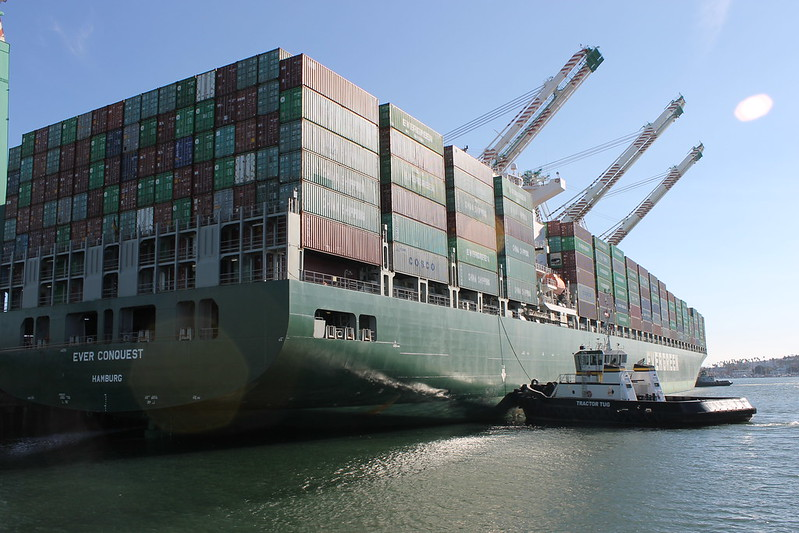
\includegraphics[width=0.5\textwidth,height=\textheight]{img/11102039694_d42ca1ff1c_c.jpg}

}

\subcaption{\label{fig-ship}Containershiff mit vielen Paketen, Corey
Seeman, CC-BY-NC 20, Flickr.com}

\subsection{Es kommen viele dazu}

\centering{

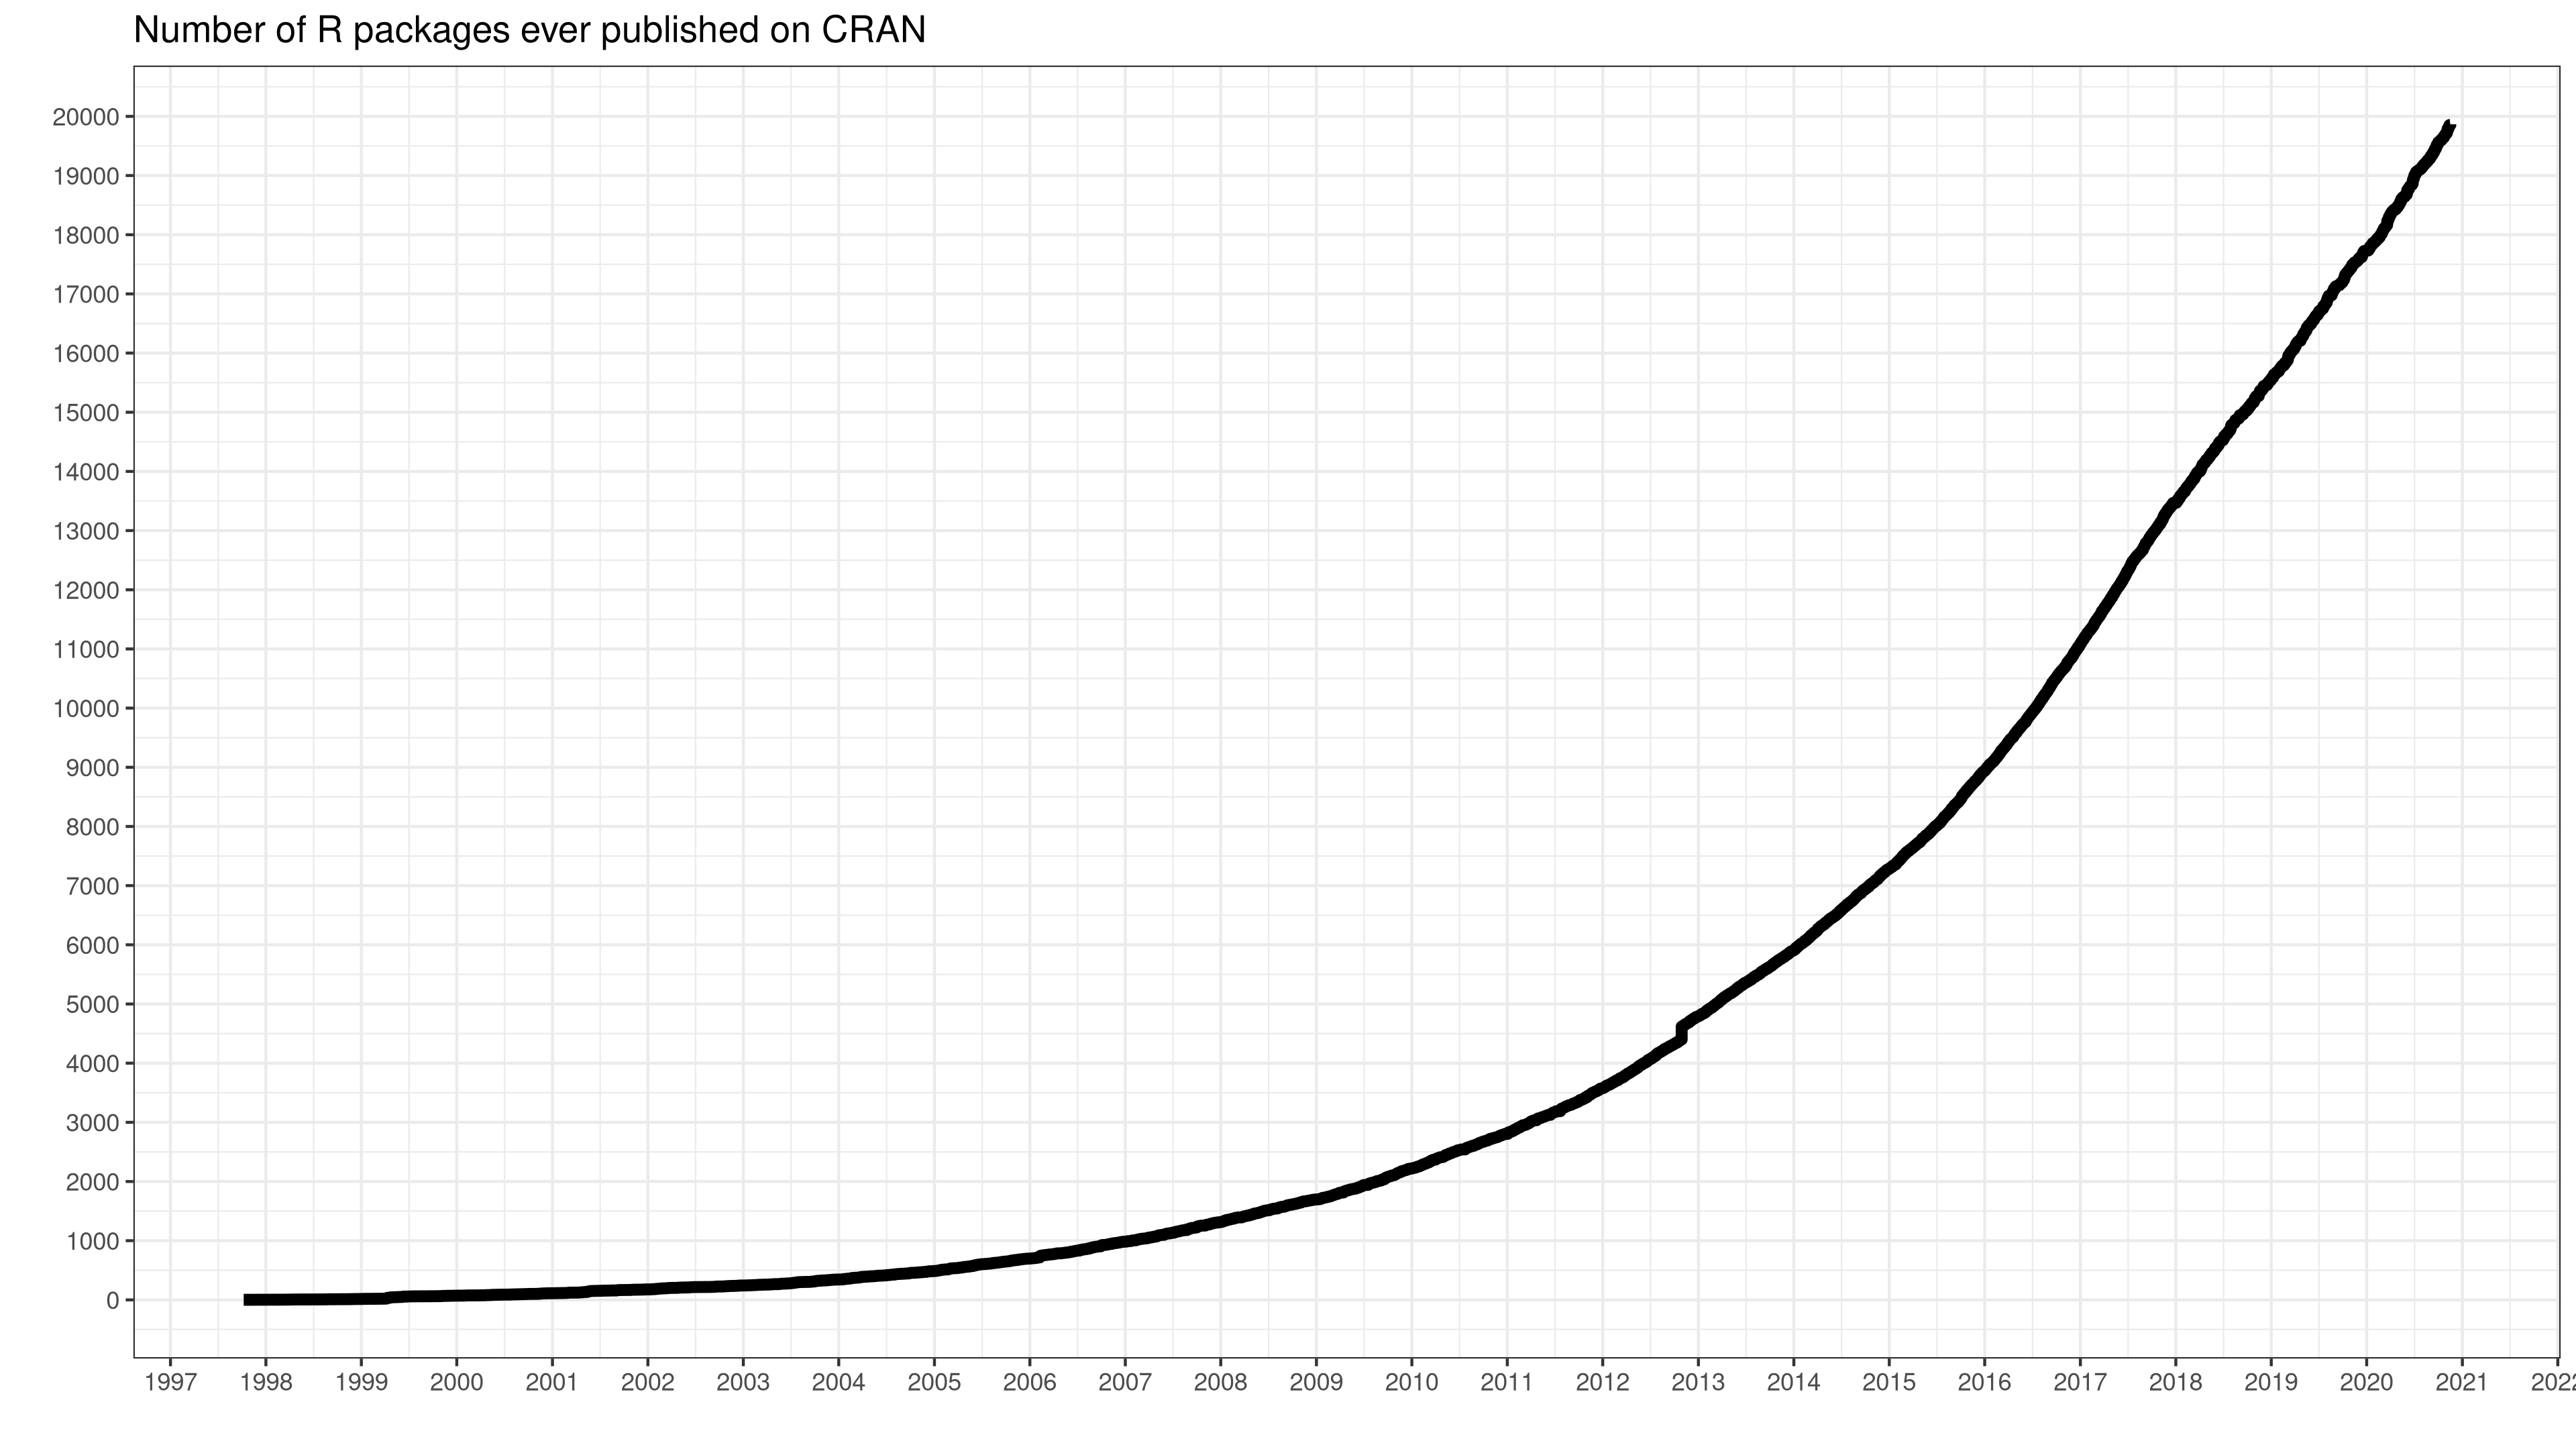
\includegraphics{img/number-of-submitted-packages-to-CRAN.png}

}

\subcaption{\label{fig-cran}Die Anzahl der R-Pakete ist exponenziell
gewachsen}

Es gibt viele R-Pakete.

}

\caption{\label{fig-pakete}}

\end{figure}%

\emph{Erweiterungen} kennt man von vielen Programmen, sie werden auch
\emph{Add-Ons}, \emph{Plug-Ins} oder sonstwie genannt. Man siehe zur
Verdeutlichung Erweiterungen beim Broswer Chrome,
Abbildung~\ref{fig-chrome}.

\begin{figure}

\centering{

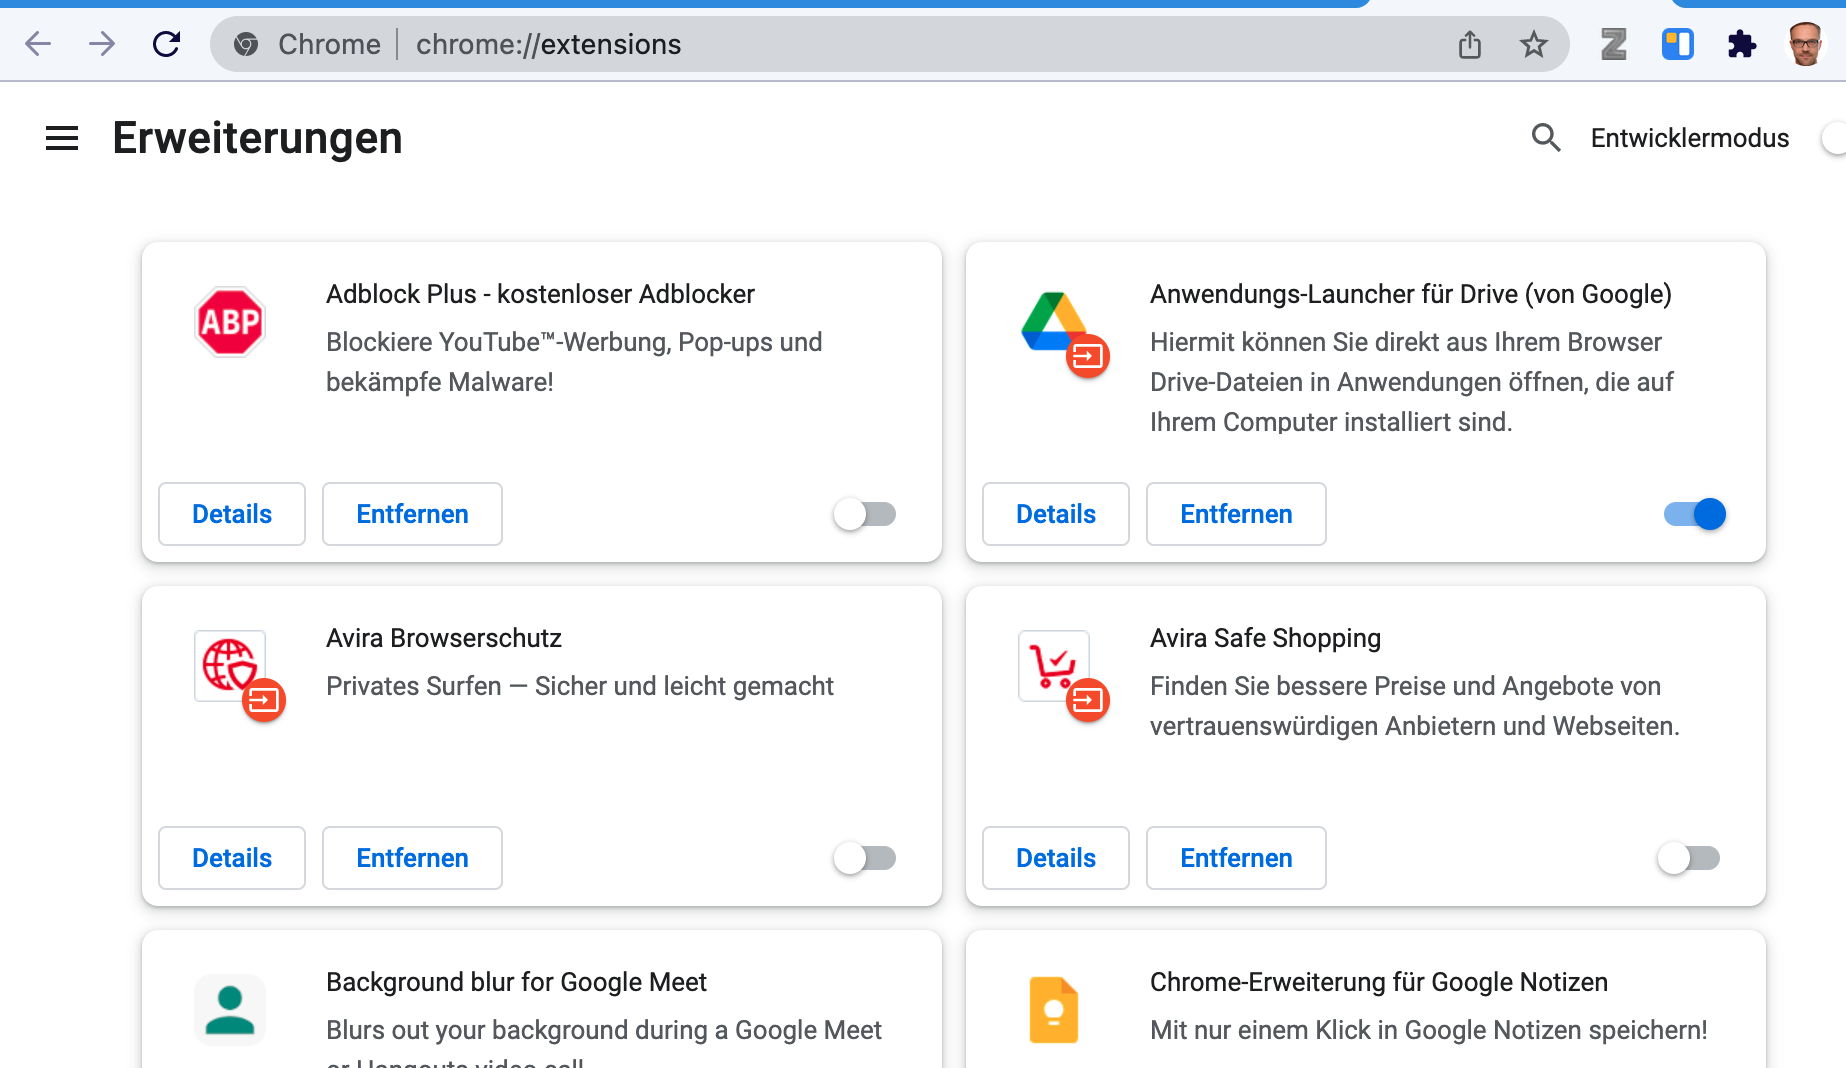
\includegraphics[width=0.5\textwidth,height=\textheight]{img/chrome-extensions.png}

}

\caption{\label{fig-chrome}Erweiterungen beim Browser Chrome}

\end{figure}%

Die Anzahl der R-Pakete ist groß; allein auf dem ``offiziellen
Web-Store'' (nennt sich ``CRAN'') von R gibt es ca. 20,000 Pakete (vgl.
Abbildung~\ref{fig-cran});
\href{https://gist.github.com/daroczig/3cf06d6db4be2bbe3368}{Stand:
2022; Quelle}). Und es kommen immer mehr dazu.

\subsection{Pakete installieren}\label{install-r-pckgs}

Wie jede Software muss man Pakete (Erweiterungen für R) erst einmal
installieren, bevor man sie verwenden kann. Ja, einmal installieren
reicht.

Das geht komfortabel, wenn man beim Reiter \emph{Packages} auf
\emph{Install} klickt (s. Abbildung~\ref{fig-pckgs}) und dann den Namen
des zu installierenden Pakets eingibt.

\begin{figure}

\begin{minipage}{0.50\linewidth}

\centering{

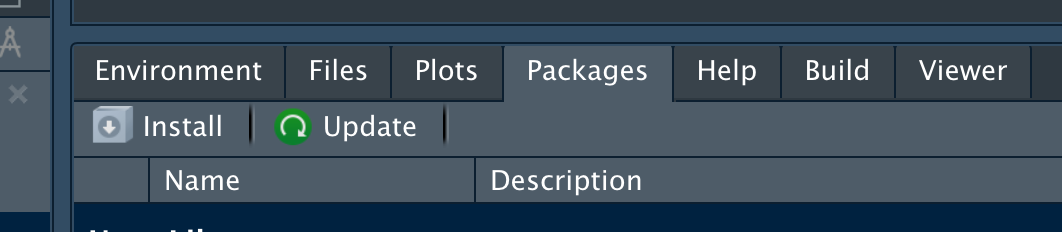
\includegraphics{img/install-packages.png}

}

\subcaption{\label{fig-install-packages}Klicken Sie auf ``Install'' im
Reiter ``Packages'', um R-Pakete zu installieren}

\end{minipage}%
%
\begin{minipage}{0.50\linewidth}

\end{minipage}%
\newline
\begin{minipage}{0.50\linewidth}

\centering{

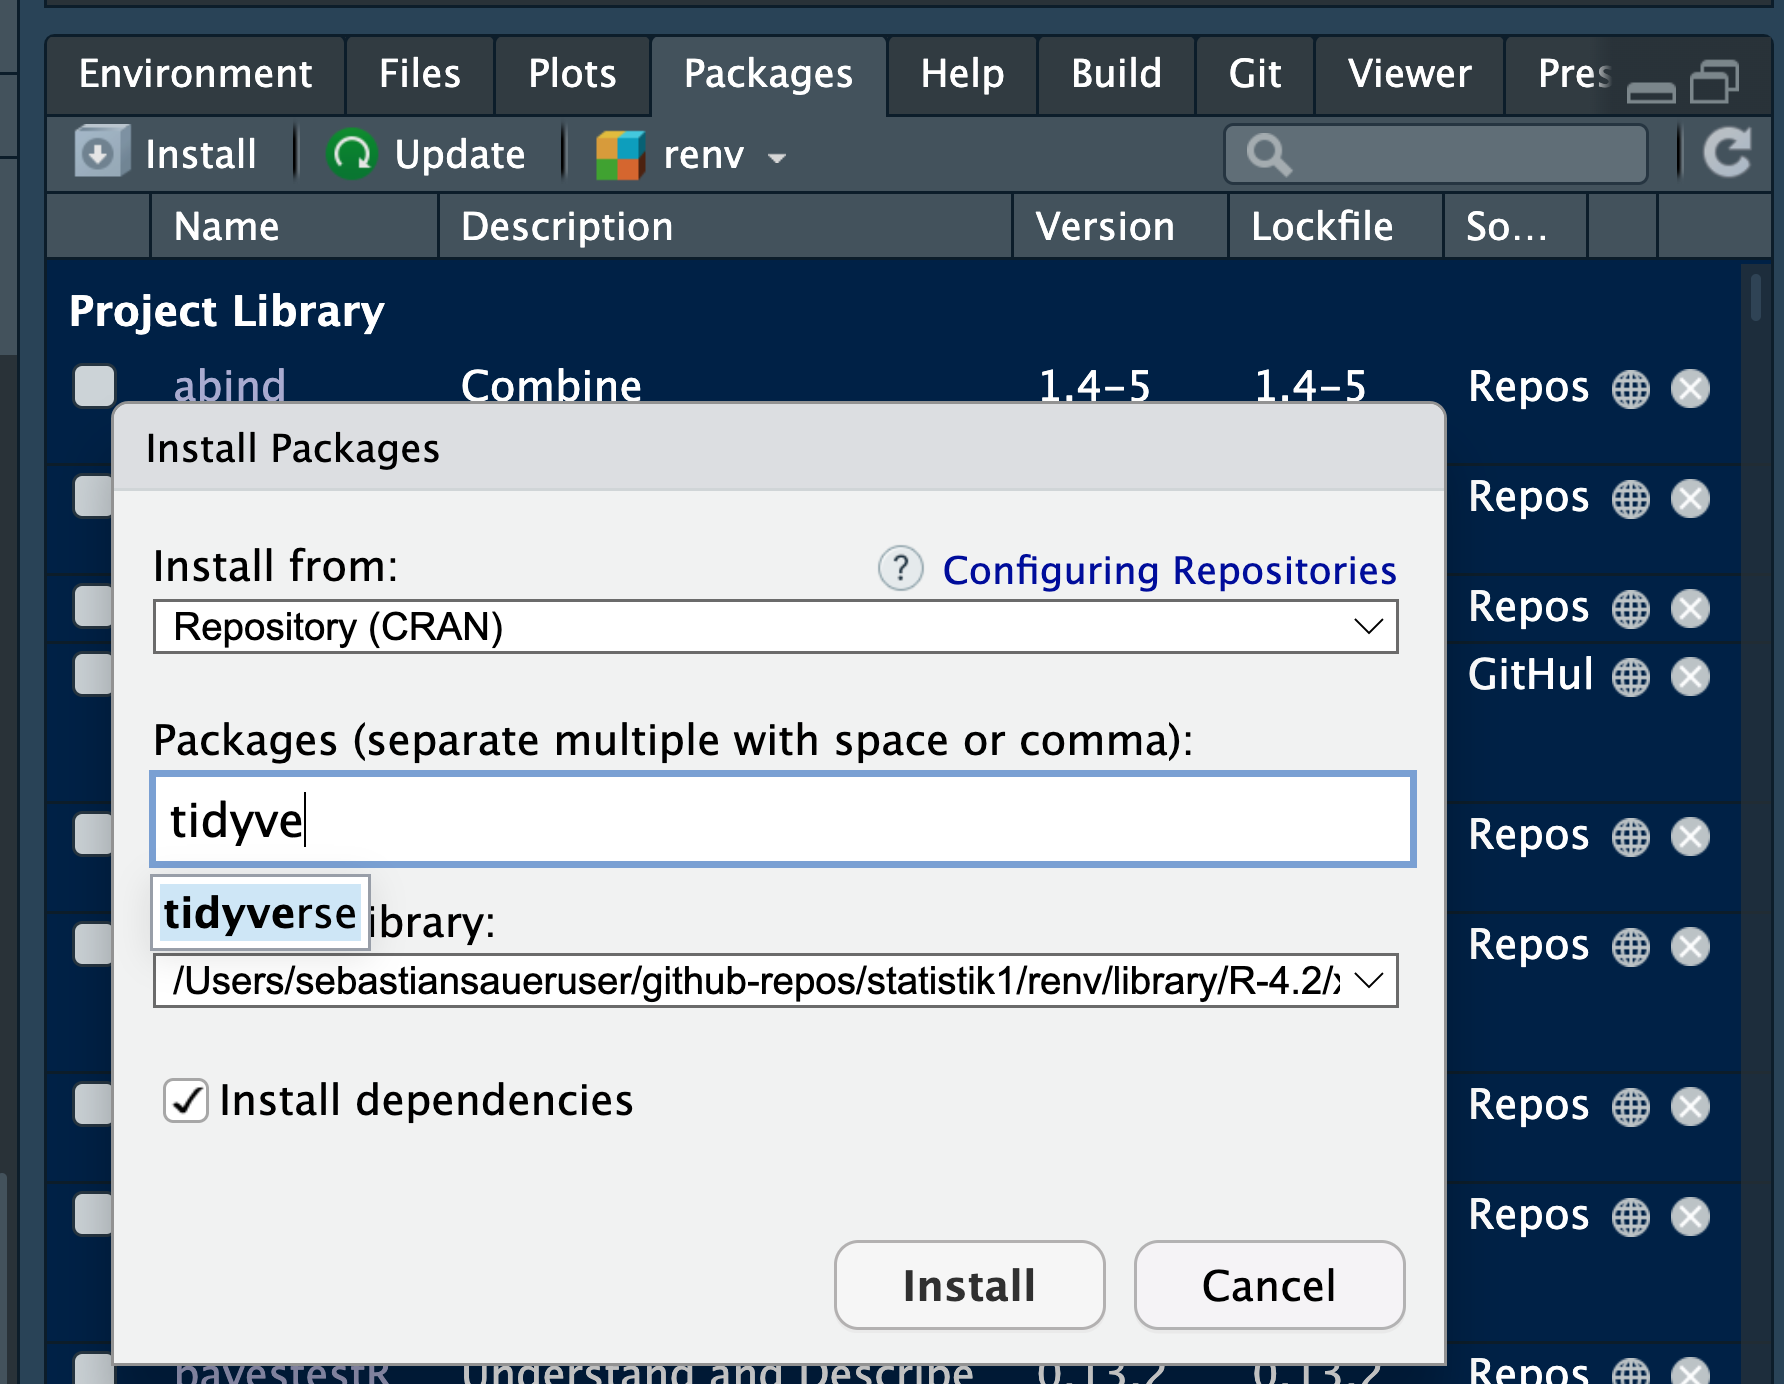
\includegraphics{img/install-packages3.png}

}

\subcaption{\label{fig-so-installieren}So kann man R-Pakete installieren
in RStudio}

\end{minipage}%

\caption{\label{fig-pckgs}So installiert man Pakete in R.}

\end{figure}%

Dann öffnet sich ein Menü, wo man die Namen der gewünschten R-Pakete
eingeben kann (s. Abbildung Abbildung~\ref{fig-install-packages2}).

\begin{figure}

\centering{

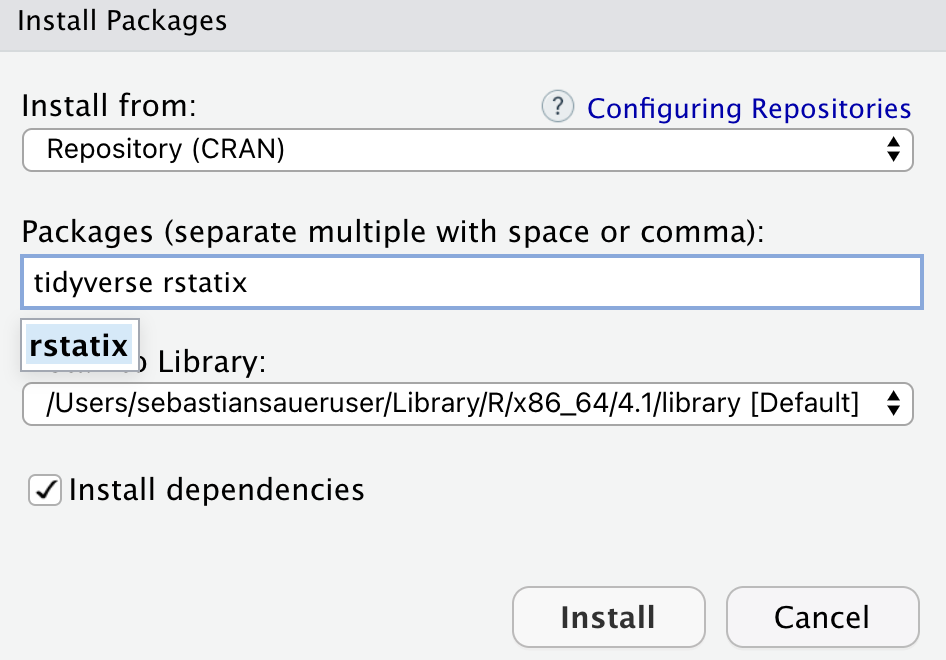
\includegraphics[width=0.25\textwidth,height=\textheight]{img/install-packages2.png}

}

\caption{\label{fig-install-packages2}Hier den oder die Namen der
gewünschten R-Pakete eingeben}

\end{figure}%

\begin{quote}
🧑‍🎓Welche R-Pakete sind denn schon installiert?
\end{quote}

Im Reiter \emph{Packages} können Sie nachschauen, welche Pakete auf
Ihrem Computer schon installiert sind. Diese Pakete brauchen Sie
logischerweise dann \emph{nicht} noch mal installieren, s.
Abbildung~\ref{fig-paket-installiert}.

\begin{figure}

\centering{

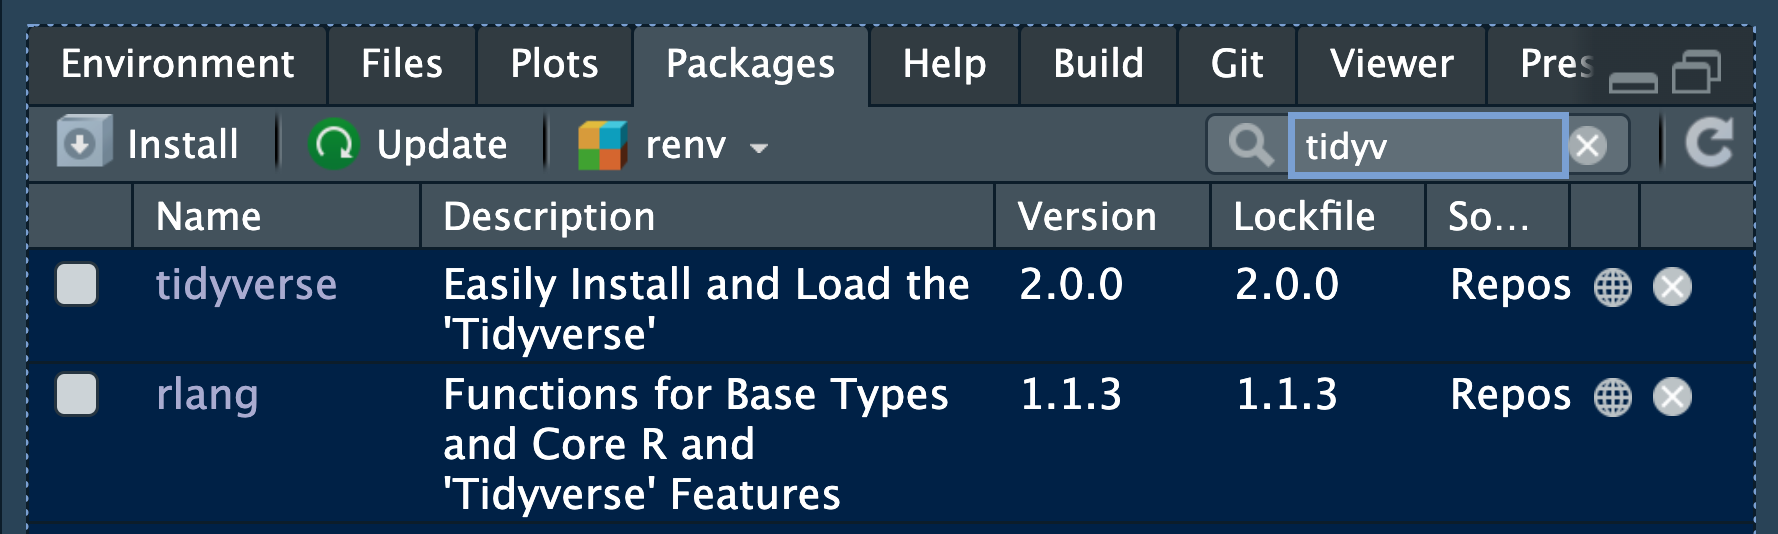
\includegraphics{img/paket-installiert.png}

}

\caption{\label{fig-paket-installiert}So sehen Sie, ob ein R-Paket auf
Ihrem System installiert ist}

\end{figure}%

\begin{quote}
🧑‍🎓Ja, aber welche R-Pakete ``soll'' ich denn installieren, welche brauch
ich denn?
\end{quote}

Im Moment sollten Sie die folgenden Pakete installiert haben:

\begin{itemize}
\tightlist
\item
  \texttt{tidyverse}
\item
  \texttt{easystats}
\end{itemize}

Wenn Sie die noch nicht installiert haben sollten, dann können Sie das
jetzt ja nachholen.\footnote{Übrigens sind \texttt{tidyverse} und
  \texttt{easystats} Pakete, die nur dafür da sind, mehrere Pakete zu
  installieren. So gehören z.B. zu \texttt{tidyverse} die Pakete
  \texttt{ggplot} (Daten verbildlichen) und \texttt{dplyr} (Datenjudo).
  Damit wir nicht alle Pakete einzeln installieren und starten müssen,
  bietet uns das Paket \texttt{tidyverse} den Komfort, alle die Pakete
  dieser ``Sammlung'' auf einmal zu starten. Praktisch.}

\begin{tcolorbox}[enhanced jigsaw, colback=white, opacityback=0, arc=.35mm, titlerule=0mm, breakable, toptitle=1mm, colframe=quarto-callout-caution-color-frame, title=\textcolor{quarto-callout-caution-color}{\faFire}\hspace{0.5em}{Vorsicht}, rightrule=.15mm, colbacktitle=quarto-callout-caution-color!10!white, coltitle=black, leftrule=.75mm, bottomrule=.15mm, bottomtitle=1mm, opacitybacktitle=0.6, toprule=.15mm, left=2mm]

Bevor Sie ein R-Paket (oder überhaupt irgendwelche Software)
installieren/updaten, sollten Sie das R-Paket schließen/beenden. Sonst
schrauben Sie an einem elektrischen Gerät herum, das noch unter Strom
steht (nicht gut). Die einfachste Art, alle Pakete zu beenden ist,
\texttt{Session\ \textgreater{}\ Restart\ R} zu klicken (in
RStudio).\(\square\)

\end{tcolorbox}

\subsection{Pakete starten}\label{pakete-starten}

Wenn Sie ein Softwareprogramm - nichts anderes sind R-Pakete -
installiert haben, müssen Sie es noch \emph{starten}.

Merke: Ein bestimmtes R-Paket muss man nur \emph{einmalig installieren}.
Aber man muss es \emph{jedes Mal neu starten}, wenn man R (bzw. RStudio)
startet.

Sie erkennen leicht, ob ein Paket gestartet ist, wenn Sie ein Häkchen
vor dem Namen des Pakets in der Paketliste (Reiter \emph{Packages})
sehen, s. Abbildung Abbildung~\ref{fig-install-packages}.\footnote{Dieses
  Video
  \url{https://www.youtube.com/watch?v=Yej9xzKQ3yI&list=PLRR4REmBgpIEaIyeNBgNGPgmhQJ_T1y8_&index=26}
  verdeutlicht den Unterschied zwischen \emph{Installation} und
  \emph{Starten} eines R-Pakets.}

\section{Mit R arbeiten}\label{mit-r-arbeiten}

\subsection{Projekte in R}\label{projekte-in-r}

Ein \emph{Projekt} in RStudio (s. Abbildung~\ref{fig-projects}) ist
letztlich ein Ordner, der als ``Basis'' für eine Reihe von Dateien
verwendet wird. Sagen wir, das Projekt heißt \texttt{cool\_stuff}.
RStudio legt uns diesen Ordner an einem von uns gewählten Platz auf
unserem Computer an. Das ist ganz praktisch, weil man dann sagen kann
``Hey R, nimmt die Datei `daten.csv'\,'', ohne einen Pfad anzugeben.
Vorausgesetzt, die Datei liegt auch im Projektordner
(\texttt{cool\_stuff}).

Projekte kann anlegen mit Klick auf das Icon, das einen Quader mit dem
Buchstaben R darin anzeigt (s. Abbildung~\ref{fig-rstudio-projekte}).
RStudio-Projekte machen Ihr Leben leichter (s.
Abbildung~\ref{fig-projects}).

\begin{figure}

\begin{minipage}{0.50\linewidth}

\centering{

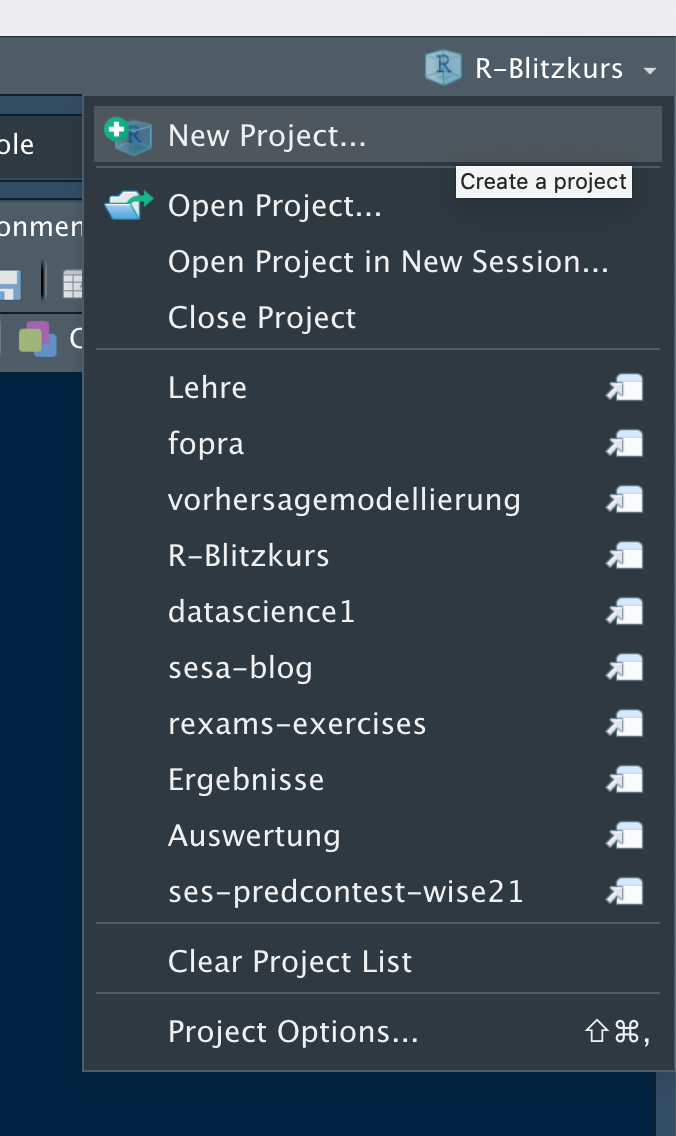
\includegraphics[width=0.5\textwidth,height=\textheight]{img/rstudio-projekte.png}

}

\subcaption{\label{fig-rstudio-projekte}RStudio-Projekte, Beispiele}

\end{minipage}%
%
\begin{minipage}{0.50\linewidth}

\centering{

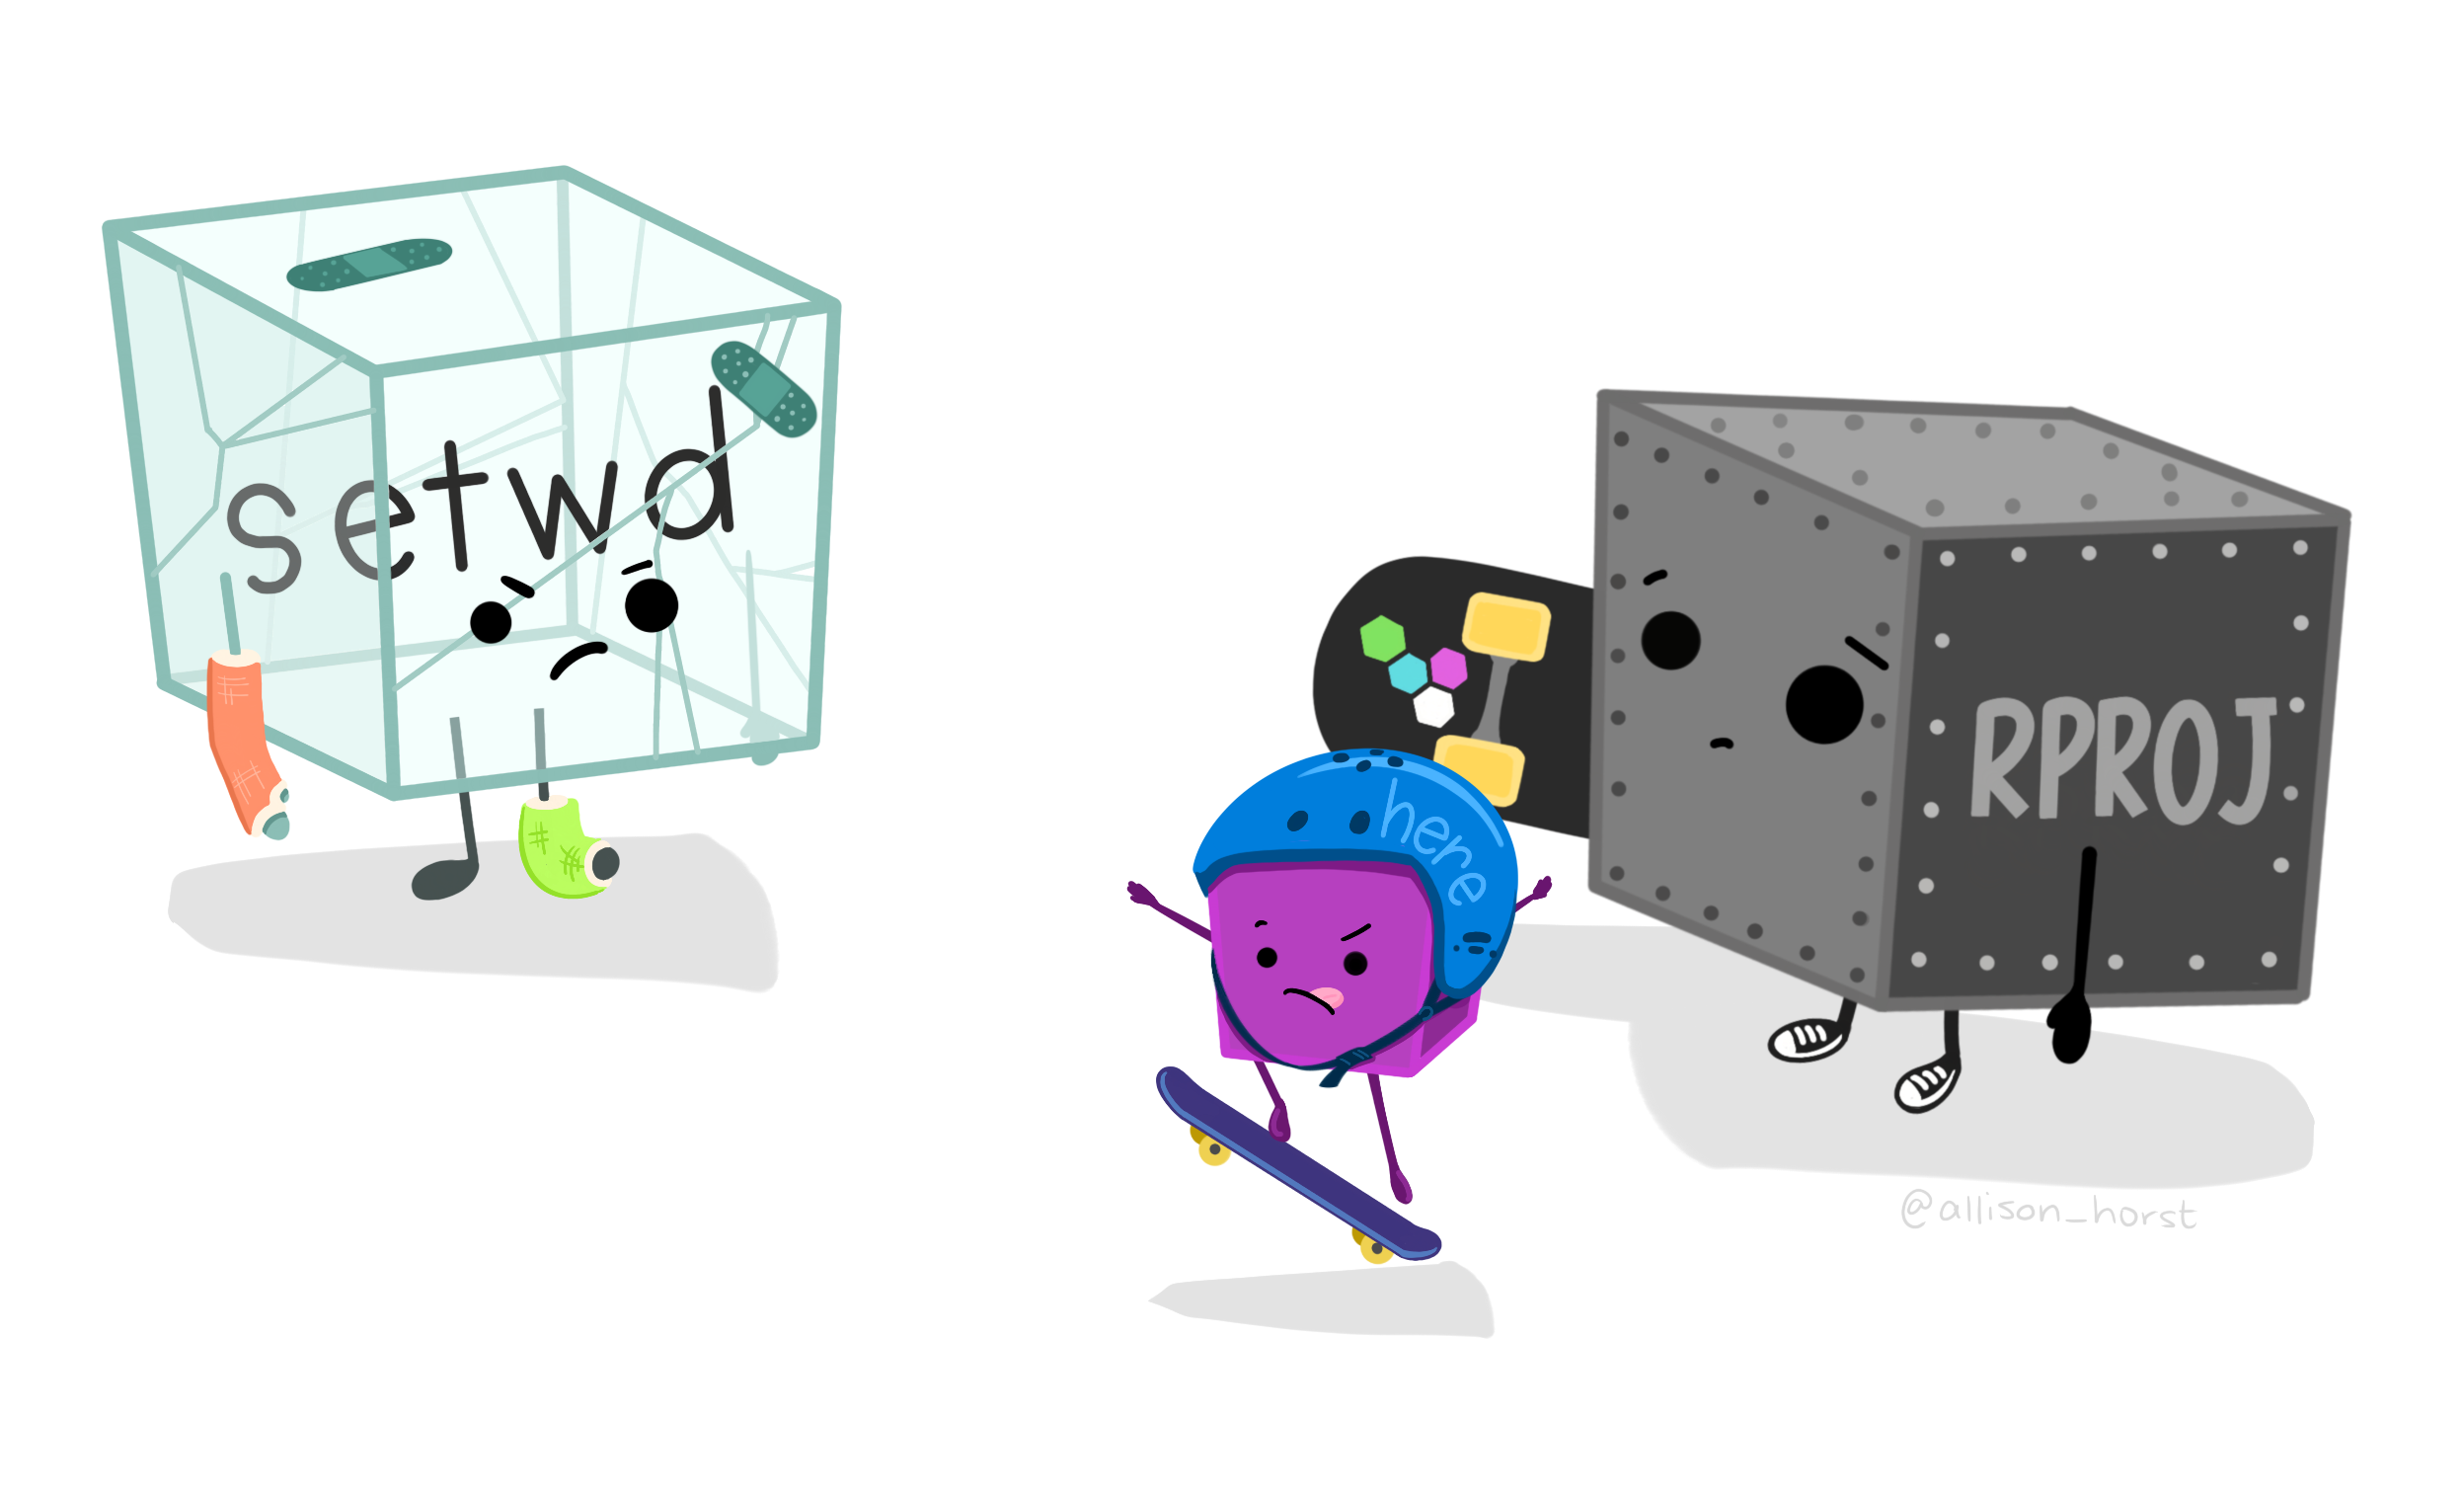
\includegraphics{img/cracked_setwd.png}

}

\subcaption{\label{fig-setwd}RStudio-Projekte sind viel sicherer als das
Arbeitsverzeichnis von Hand zu wählen oder mit Pfaden herumzubasteln.
Image credit: Allision Horst}

\end{minipage}%

\caption{\label{fig-projects}Nutzen Sie RStudio-Projekte, das macht Ihr
Leben leichter.}

\end{figure}%

\subsection{Skriptdateien}\label{skriptdateien}

Die R-Befehle (``Syntax'') schreiben Sie am besten in eine speziell
dafür vorgesehene Textdatei in RStudio. Eine Sammlung von
(R-)Computer-Befehlen nennt man auch ein \emph{Skript}, daher spricht
man auch von einer \emph{Skriptdatei}.

\subsubsection{So öffnen Sie eine neue
Skriptdatei}\label{so-uxf6ffnen-sie-eine-neue-skriptdatei}

Um eine neue R-Skriptdatei zu öffnen, klicken Sie auf das Icon, das ein
weißes Blatt mit einem grünen Pluszeichen zeigt, s.
Abbildung~\ref{fig-script-new}.

\begin{figure}

\begin{minipage}{0.50\linewidth}

\centering{

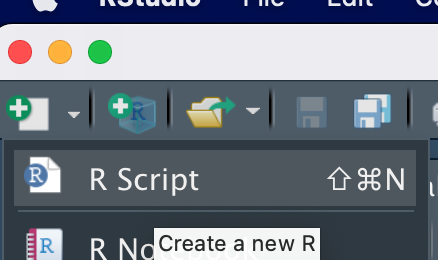
\includegraphics[width=0.5\textwidth,height=\textheight]{img/script-new.png}

}

\subcaption{\label{fig-script-new1}So erstellen Sie eine neue
Skriptdatei}

\end{minipage}%
%
\begin{minipage}{0.50\linewidth}

\end{minipage}%
\newline
\begin{minipage}{0.50\linewidth}

\end{minipage}%

\caption{\label{fig-script-new}Es gibt verschiedene Wege, um eine neue
R-Skript-Datei in RStudio zu öffnen.}

\end{figure}%

\subsubsection{So speichern Sie Ihre
Skripdatei}\label{so-speichern-sie-ihre-skripdatei}

Vergessen Sie nicht zu \emph{speichern}, wenn Sie ein tolles Skript
geschrieben haben. Dafür gibt es mehrere Möglichkeiten:

\begin{enumerate}
\def\labelenumi{\arabic{enumi}.}
\tightlist
\item
  Strg+S
\item
  Menü: File \textgreater{} Save
\item
  Klick auf das Icon mit der Diskette, s.
  Abbildung~\ref{fig-script-new}.
\end{enumerate}

\subsubsection{So öffnen Sie eine
Skriptdatei}\label{so-uxf6ffnen-sie-eine-skriptdatei}

Eine Skriptdatei können Sie in typischer Manier \emph{öffnen}:

\begin{enumerate}
\def\labelenumi{\arabic{enumi}.}
\tightlist
\item
  Strg+O
\item
  Klick auf das Icon mit der Akte und dem grünen Pfeil (vgl.
  Abbildung~\ref{fig-script-new})
\item
  Menü: \texttt{File\ \textgreater{}\ Open\ File...}
\end{enumerate}

\subsection{Quarto-Dokumente}\label{quarto-dokumente}

\href{https://quarto.org/}{Quarto} ist ein Programm zum Erstellen von
Texten, in das man R-Syntax einfügen kann. Die Ausgaben der R-Befehle
werden dann direkt im Dokument eingebunden.
Abbildung~\ref{fig-exm-quarto} zeit ein Beispiel für ein
Quarto-Dokument.

\begin{tcolorbox}[enhanced jigsaw, colback=white, opacityback=0, arc=.35mm, titlerule=0mm, breakable, toptitle=1mm, colframe=quarto-callout-note-color-frame, title=\textcolor{quarto-callout-note-color}{\faInfo}\hspace{0.5em}{Hinweis}, rightrule=.15mm, colbacktitle=quarto-callout-note-color!10!white, coltitle=black, leftrule=.75mm, bottomrule=.15mm, bottomtitle=1mm, opacitybacktitle=0.6, toprule=.15mm, left=2mm]

Quarto ist eine komfortable und leistungsfähige Methode, um Dokumente
mit R-Syntax zu schreiben. Sie sind aber nicht verpflichtet, Quarto zu
nutzen. Stattdessen können Sie Ihre Syntax auch in Skriptdateien
schreiben. \(\square\)

\end{tcolorbox}

\begin{figure}

\centering{

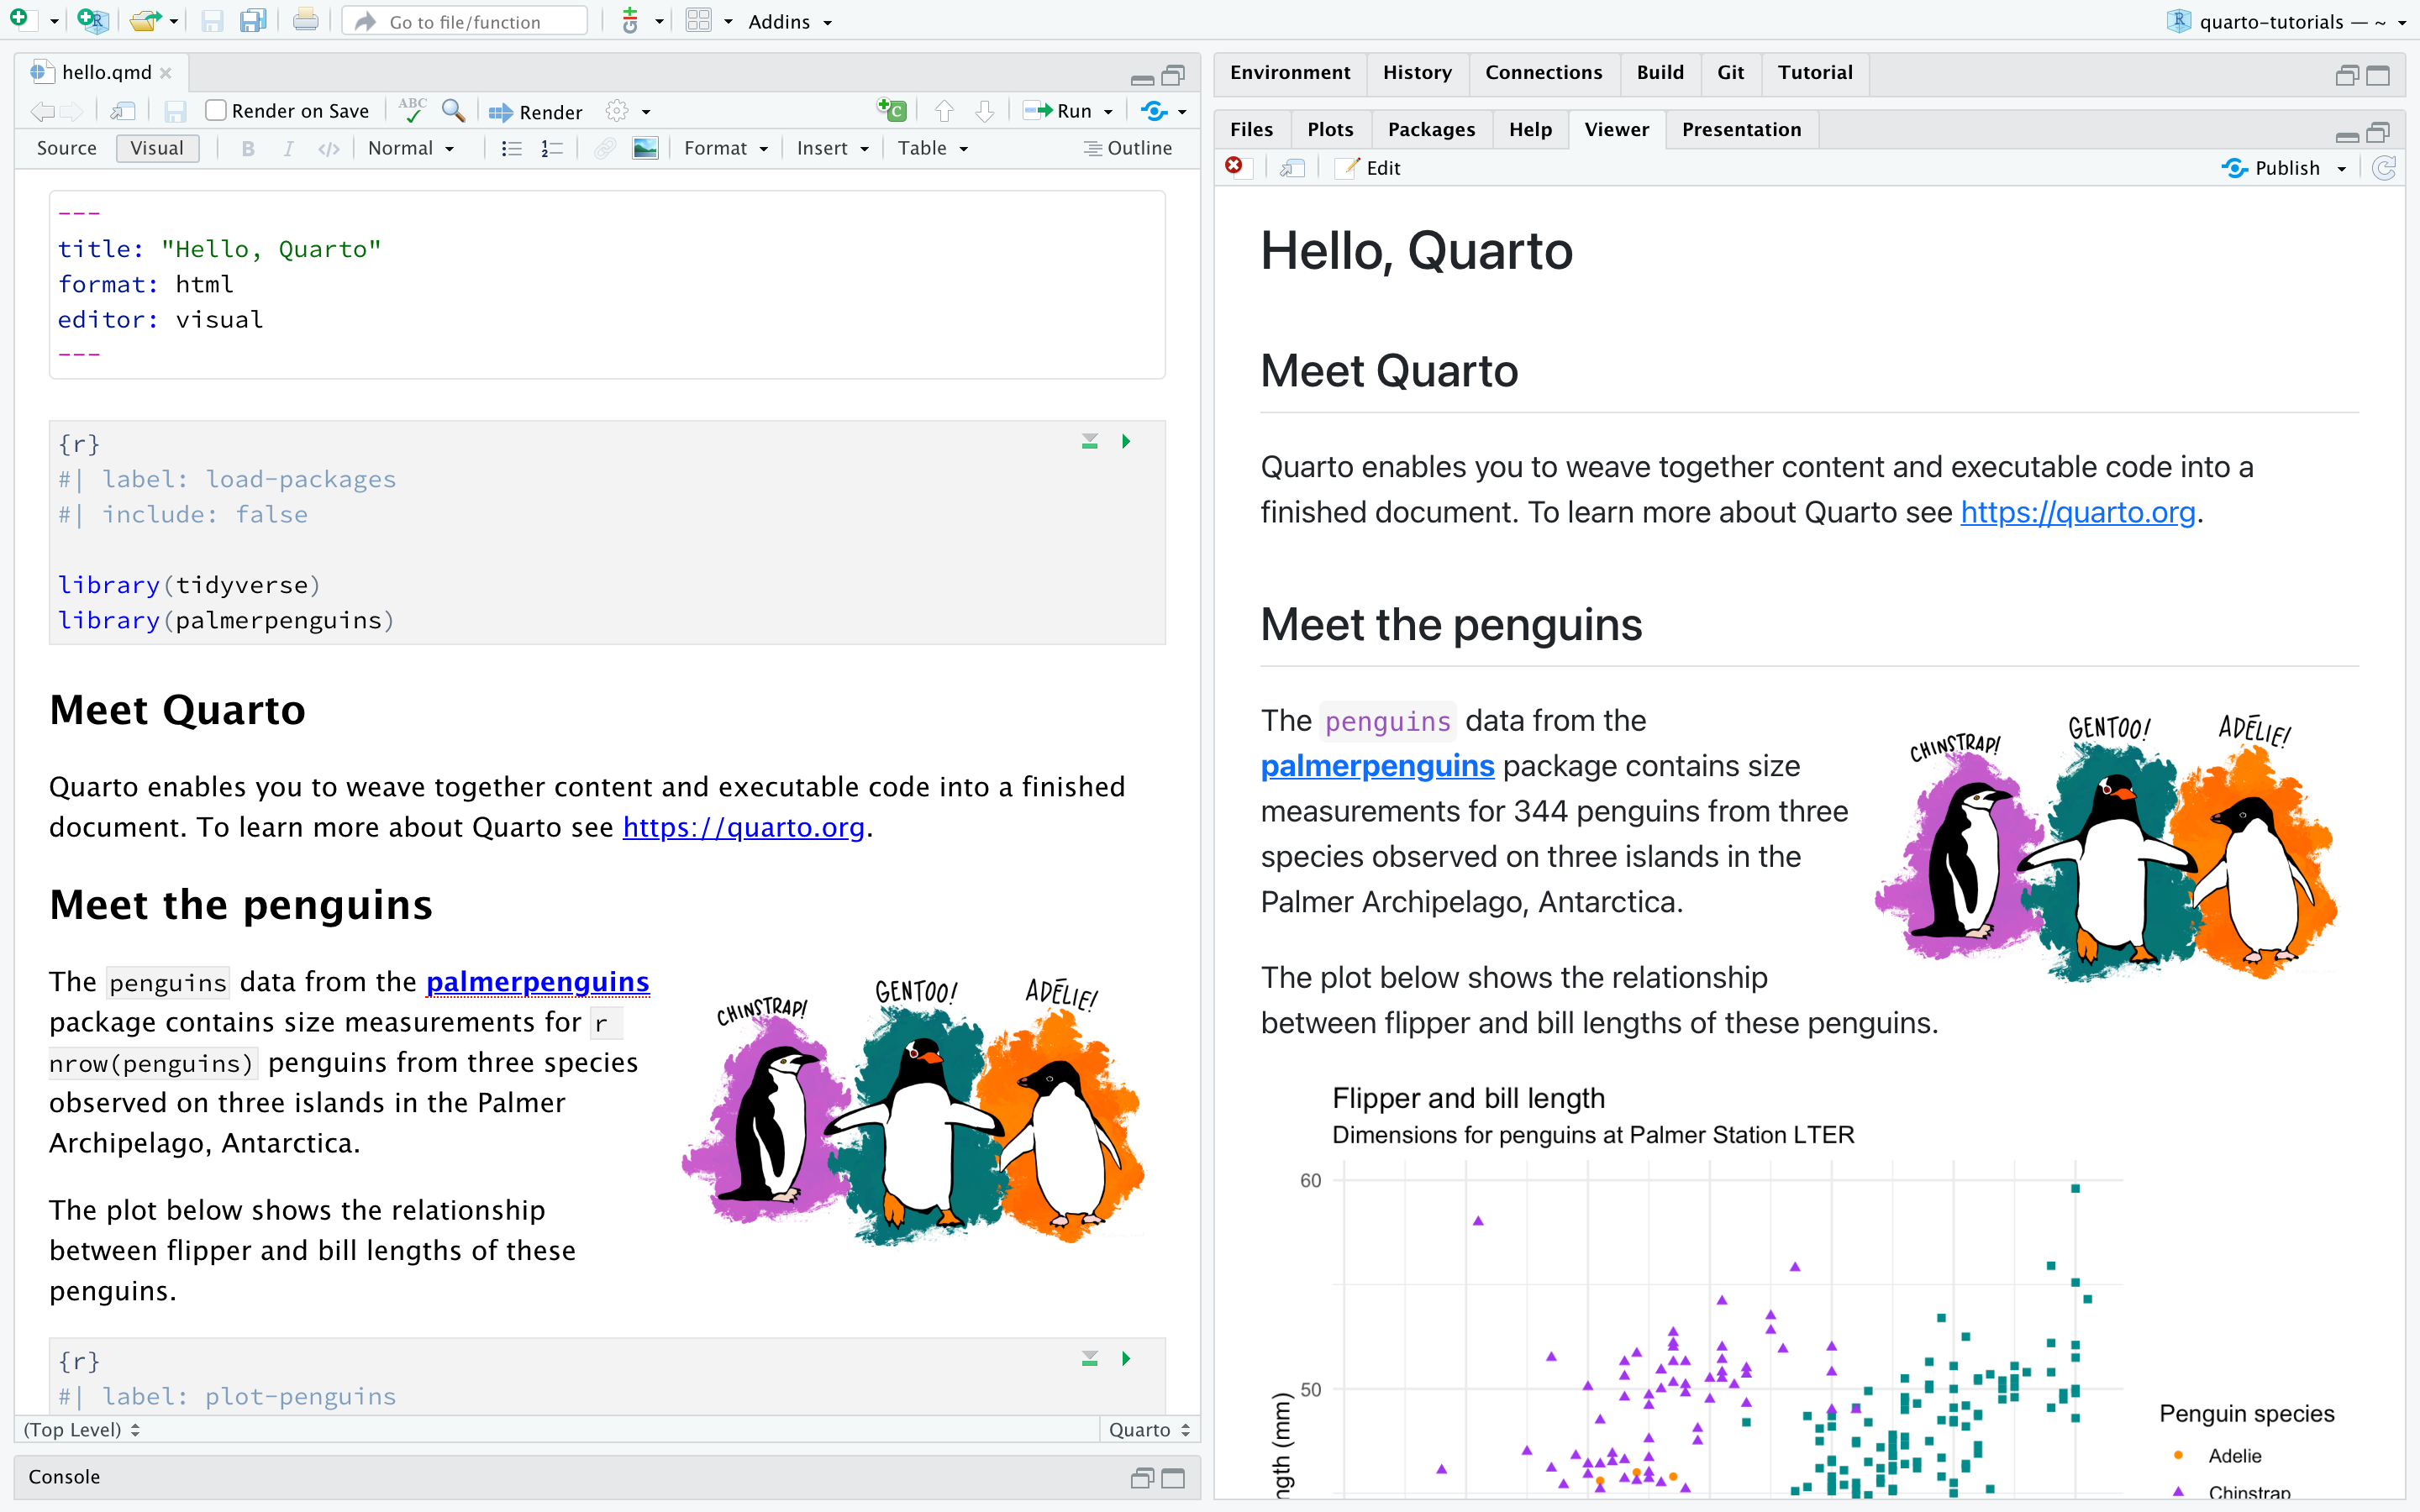
\includegraphics{index_files/mediabag/rstudio-hello.png}

}

\caption{\label{fig-exm-quarto}Dokumente schreiben mit Quarto}

\end{figure}%

Wenn Sie Quarto nutzen möchten, müssen Sie es zunächst installieren,
d.h. \href{https://quarto.org/docs/get-started/}{herunterladen}. Dann
können Sie in RStudio Quarto-Dateien erstellen.\footnote{\textless ttps://quarto.org/docs/get-started/\textgreater{}}
Ein neues Quarto-Dokument können Sie erstellen mit Klick auf \emph{File
\textgreater{} New File \textgreater{} Quarto Document
\ldots{}}.\footnote{Dieses Video \url{https://youtu.be/_f3latmOhew} gibt
  Ihnen Einstiegshilfe in Quarto.}

\section{Errisch für Einsteiger}\label{errisch-fuxfcr-einsteiger}

\begin{tcolorbox}[enhanced jigsaw, colback=white, opacityback=0, arc=.35mm, titlerule=0mm, breakable, toptitle=1mm, colframe=quarto-callout-caution-color-frame, title=\textcolor{quarto-callout-caution-color}{\faFire}\hspace{0.5em}{Vorsicht}, rightrule=.15mm, colbacktitle=quarto-callout-caution-color!10!white, coltitle=black, leftrule=.75mm, bottomrule=.15mm, bottomtitle=1mm, opacitybacktitle=0.6, toprule=.15mm, left=2mm]

R ist penibel: So sind \texttt{name} und \texttt{Name} zwei verschiedene
Variablen für R. Groß- und Kleinschreibung wird von R streng beachtet!
Hingegen ist es R egal, ob Sie zur besseren Übersichtlichkeit
Leerzeichen in Ihre Syntax tippen. Ausnahme sind spezielle Operatoren
wie \texttt{\textless{}-} oder \texttt{\textless{}=}.

Eine gute Nachricht: Wenn R etwas von \texttt{WARNING} (bzw. Warnung)
sagt, können Sie das zumeist ignorieren. Eine \emph{Warnung} ist kein
Fehler (\texttt{ERROR}) und meistens nicht gravierend oder nicht
dringend. Ihre Syntax läuft trotzdem durch. Im Zweifel ist Googeln eine
gute Idee. Nur wenn R von \texttt{Error} spricht, ist es auch ein Fehler
und Ihre Syntax läuft nicht durch.\(\square\)

\end{tcolorbox}

\subsection{Variablen}\label{sec-rvars}

In jeder Programmiersprache kann man Variablen definieren, so auch in R:

\begin{Shaded}
\begin{Highlighting}[]
\NormalTok{richtige\_antwort }\OtherTok{=} \DecValTok{42}
\NormalTok{falsche\_antwort }\OtherTok{=} \DecValTok{43}
\NormalTok{typ }\OtherTok{=} \StringTok{"Antwort"}
\NormalTok{ist\_korrekt }\OtherTok{=} \ConstantTok{TRUE}
\end{Highlighting}
\end{Shaded}

Alternativ zum Gleichheitszeichen \texttt{=} können Sie auch (synonym)
den Zuweisungspfeil \texttt{\textless{}-} verwenden. Beides führt zum
gleichen Ergebnis. Allerdings ist der Zuweisungspfeil präziser, und
sollte daher \emph{bevorzugt} werden.

Der \emph{Zuweisungspfeil} \texttt{\textless{}-} bzw. das
Gleichheitszeichen \texttt{=} definiert eine neue \emph{Variable} (oder
überschreibt den Inhalt, wenn die Variable schon existiert).\footnote{Dieses
  Video
  \url{https://www.youtube.com/watch?v=TKQk-tEF9YQ&list=PLRR4REmBgpIEaIyeNBgNGPgmhQJ_T1y8_&index=28}
  und dieses Video
  \url{https://www.youtube.com/watch?v=Nal0m_AmMwg&list=PLRR4REmBgpIEaIyeNBgNGPgmhQJ_T1y8_&index=48}
  geben eine Einführung in das Definieren von Variablen in R}.

\begin{Shaded}
\begin{Highlighting}[]
\NormalTok{richtige\_antwort }\OtherTok{\textless{}{-}} \DecValTok{42}
\NormalTok{falsche\_antwort }\OtherTok{\textless{}{-}} \DecValTok{43}
\NormalTok{typ }\OtherTok{\textless{}{-}} \StringTok{"Antwort"}
\NormalTok{ist\_korrekt }\OtherTok{\textless{}{-}} \ConstantTok{TRUE}
\end{Highlighting}
\end{Shaded}

Sie können sich eine Variable wie einen Becher oder Behälter vorstellen,
der bestimmte Werte enthält. Auf dem Becher steht (mit Edding
geschrieben) der Name des Bechers. Natürlich können Sie die Werte aus
dem Becher entfernen und sie durch neue ersetzen (vgl.
Abbildung~\ref{fig-def-vars}).

\begin{figure}

\centering{

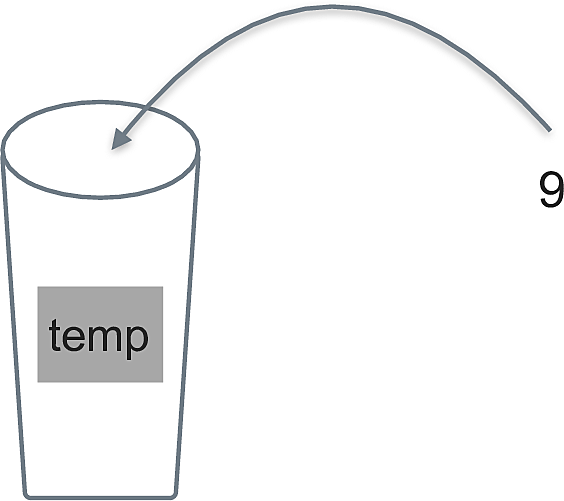
\includegraphics[width=0.25\textwidth,height=\textheight]{img/Variablen_zuweisen.png}

}

\caption{\label{fig-def-vars}Variablen zuweisen}

\end{figure}%

R kann übrigens auch rechnen. Probieren Sie es doch gleich mal hier aus!

\begin{Shaded}
\begin{Highlighting}[]
\NormalTok{die\_summe }\OtherTok{\textless{}{-}}\NormalTok{ falsche\_antwort }\SpecialCharTok{+}\NormalTok{ richtige\_antwort}
\end{Highlighting}
\end{Shaded}

Aber was ist jetzt der Wert, der ``Inhalt'' der Variable
\texttt{die\_summe}?

Um den Wert, d.h. den Inhalt einer Variablen in R \emph{auszulesen},
geben wir einfach den Namen des Objekts ein:

\begin{Shaded}
\begin{Highlighting}[]
\NormalTok{die\_summe}
\DocumentationTok{\#\# [1] 85}
\end{Highlighting}
\end{Shaded}

Was passiert wohl, wenn wir \texttt{die\_summe} jetzt wie folgt
definieren?

\begin{Shaded}
\begin{Highlighting}[]
\NormalTok{die\_summe }\OtherTok{\textless{}{-}}\NormalTok{ falsche\_antwort }\SpecialCharTok{+}\NormalTok{ richtige\_antwort }\SpecialCharTok{+} \DecValTok{1}
\end{Highlighting}
\end{Shaded}

Wer hätt's geahnt:

\begin{Shaded}
\begin{Highlighting}[]
\NormalTok{die\_summe}
\DocumentationTok{\#\# [1] 86}
\end{Highlighting}
\end{Shaded}

Variablen können auch ``leer'' sein:

\begin{Shaded}
\begin{Highlighting}[]
\NormalTok{alter }\OtherTok{\textless{}{-}} \ConstantTok{NA}
\NormalTok{alter}
\DocumentationTok{\#\# [1] NA}
\end{Highlighting}
\end{Shaded}

\texttt{NA} steht für \emph{not available}, nicht verfügbar und macht
deutlich, dass hier ein Wert fehlt.

\begin{quote}
🧑‍🎓 Wozu brauche ich bitte fehlende Werte?!
\end{quote}

Fehlende Werte sind ein häufiges Problem in der Praxis. Vielleicht hat
sich die befragte Person geweigert, ihr Alter anzugeben\footnote{Datenschutz!}.
Oder als Sie die Daten in Ihren Computer eingeben wollten, ist Ihre
Katze über die Tastatur gelaufen und alles war futsch\ldots{}

\subsection{Funktionen (``Befehle'')}\label{funktionen-befehle}

Das, was R kann, ist in ``Funktionen'' hinterlegt. Genauer gesagt ist
``Befehl'' eine Funktion.

\begin{definition}[Funktion]\protect\hypertarget{def-fun}{}\label{def-fun}

Eine Funktion ist eine Regel, die jedem Eingabewert (auch Argument
genannt) einen Ausgabewert zuordnet. Man kann sich Funktionen als
Maschinen vorstellen, die Eingabedaten in Ausgabedaten umwandeln, vgl.
Abbildung~\ref{fig-function-schema}. \(\square\)

\end{definition}

\subsubsection{Eine erste Funktion: Vektoren
erstellen}\label{eine-erste-funktion-vektoren-erstellen}

Ein Beispiel für eine solche Funktion könnte sein: ``Berechne den
Mittelwert dieser Datenreihe'' (schauen wir uns gleich an).

Das geht so:

\begin{Shaded}
\begin{Highlighting}[]
\NormalTok{Antworten }\OtherTok{\textless{}{-}} \FunctionTok{c}\NormalTok{(}\DecValTok{42}\NormalTok{, }\DecValTok{43}\NormalTok{)}
\end{Highlighting}
\end{Shaded}

Der Befehl \texttt{c} (c wie \emph{c}ombine) fügt mehrere Werte zusammen
zu einer ``Liste'' (einem Vektor).\footnote{Streng genommen sollte man
  nicht von einer Liste sprechen, da es in R noch einen anderen
  Objekttyp gibt, der \texttt{list} heißt, und eine verallgemeinerte
  Form eines Vektors ist.}

\begin{definition}[]\protect\hypertarget{def-vektor}{}\label{def-vektor}

Als \emph{Vektor} bezeichnen wir eine geordnete Folge von Werten. In R
kann man sie mit der Funktion \texttt{c()} erstellen. Die Werte eines
Vektors bezeichnet man als \emph{Elemente}. \(\square\)

\end{definition}

Mit dem Zuweisungspfeil geben wir diesem Vektor einen Namen, hier
\texttt{Antworten}. Dieser Vektor besteht aus zwei Werten, zuerst
\texttt{42}, dann kommt \texttt{43}.

\begin{example}[Beispiele für
Vektoren]\protect\hypertarget{exm-vektoren}{}\label{exm-vektoren}

Vektoren können (praktisch) beliebig lang sein, z.B. drei Elemente.

\begin{Shaded}
\begin{Highlighting}[]
\NormalTok{x }\OtherTok{\textless{}{-}} \FunctionTok{c}\NormalTok{(}\DecValTok{1}\NormalTok{, }\DecValTok{2}\NormalTok{, }\DecValTok{3}\NormalTok{)}
\NormalTok{y }\OtherTok{\textless{}{-}} \FunctionTok{c}\NormalTok{(}\DecValTok{2}\NormalTok{, }\DecValTok{1}\NormalTok{, }\DecValTok{3}\NormalTok{)  }\CommentTok{\# x und y sind ungleich (Reihenfolge der Werte)}
\NormalTok{z }\OtherTok{\textless{}{-}} \FunctionTok{c}\NormalTok{(}\FloatTok{3.14}\NormalTok{, }\FloatTok{2.71}\NormalTok{)  }
\NormalTok{namen }\OtherTok{\textless{}{-}} \FunctionTok{c}\NormalTok{(}\StringTok{"Anni"}\NormalTok{, }\StringTok{"Bert"}\NormalTok{, }\StringTok{"Charli"}\NormalTok{) }\CommentTok{\# Text{-}Vektor}
\end{Highlighting}
\end{Shaded}

\end{example}

Zwei wichtige Typen von Vektoren sind numerische Vektoren (reelle
Zahlen; in R auch als \emph{numeric} oder \emph{double} bezeichnet) und
Textvektoren, in R auch als \emph{String} oder \emph{character}
bezeichnet.

\begin{example}[]\protect\hypertarget{exm-funs}{}\label{exm-funs}

Weitere Beispiel für Funktionen sind:

\begin{itemize}
\tightlist
\item
  ``Erstelle eine Liste (Vektor) von Werten''.
\item
  ``Lade dieses R-Paket.''
\item
  ``Gib den größten Wert dieser Datenreihe aus.'' \(\square\)
\end{itemize}

\end{example}

\subsection{Unsere erste statistische Funktion}\label{sec-first-fun}

Jetzt wird's ernst. Jetzt kommt die Statistik. 🧟 Berechnen wir also
unsere erste statistische Funktion: Den Mittelwert. Puh.

\begin{Shaded}
\begin{Highlighting}[]
\FunctionTok{mean}\NormalTok{(Antworten)}
\DocumentationTok{\#\# [1] 42.5}
\end{Highlighting}
\end{Shaded}

Sie hätten \texttt{Antworten} auch durch \texttt{c(42,\ 43)} ersetzen
können, so haben Sie ja schließlich die Variable gerade definiert.

R arbeitet so einen ``verschachtelten'' Befehl \emph{von innen nach
außen} ab:

Start: \texttt{mean(Antworten)}

\begin{verbatim}
  ⬇️ 
\end{verbatim}

Schritt 1: \texttt{mean(c(42,\ 43))}

\begin{verbatim}
  ⬇️ 
\end{verbatim}

Schritt 2: \texttt{42.5}

\subsubsection{Schema einer Funktion}\label{schema-einer-funktion}

Abbildung~\ref{fig-function-schema} stellt eine Funktion schematisch
dar.

\begin{figure}

\centering{

\includegraphics[width=0.5\textwidth,height=\textheight]{img/function-schema.pdf}

}

\caption{\label{fig-function-schema}Schema einer Funktion}

\end{figure}%

\subsubsection{Argumente einer Funktion}\label{argumente-einer-funktion}

Eine Funktion hat einen oder mehrere \emph{Inputs}, das sind Daten oder
Verarbeitungshinweise, die man in die Funktion \texttt{fun}
\emph{eingibt}, bevor sie loslegt. Eine Funktion hat immer (genau) eine
\emph{Ausgabe} (Output), in der das Ergebnis einer Funktion ausgegeben
wird.

\begin{definition}[Argumente einer
Funktion]\protect\hypertarget{def-args}{}\label{def-args}

Die ``Trichter'' einer (R-)Funktion, in denen man die Eingaben
``einfüllt'', nennt man auch \emph{Argumente}.\(\square\)

\end{definition}

So hat die Funktion \texttt{mean()} z.B. folgende Argumente, s.
Listing~\ref{lst-mean}.

\begin{codelisting}

\caption{\label{lst-mean}Die Argumente der R-Funktion \texttt{mean}}

\centering{

\begin{Shaded}
\begin{Highlighting}[]
\FunctionTok{mean}\NormalTok{(x, }\AttributeTok{trim =} \DecValTok{0}\NormalTok{, }\AttributeTok{na.rm =} \ConstantTok{FALSE}\NormalTok{, ...)}
\end{Highlighting}
\end{Shaded}

}

\end{codelisting}%

\begin{itemize}
\tightlist
\item
  \texttt{x}: das ist der Vektor, für den der Mittelwert berechnet
  werden soll
\item
  \texttt{trim\ =\ 0}: Sollen die extremsten Werte von \texttt{x} lieber
  ``abgeschnitten'' werden, also nicht in die Berechnung des Mittelwerts
  einfließen?
\item
  \texttt{na.rm\ =\ FALSE}: Wie soll mit fehlenden Werten \texttt{NA}
  umgegangen werden? Im Standard liefert \texttt{mean}\footnote{und
    viele andere arithmetische Funktionen in R} \texttt{NA} zurück. R
  schwenkt sozusagen die rote Fahne, um zu signalisieren, Achtung,
  Mensch, hier ist irgendwas nicht in Ordnung. Setzt man aber
  \texttt{na.rm\ =\ TRUE}, dann entfernt (remove, rm) R die fehlenden
  Werte und berechnet den Mittelwert.
\item
  \texttt{...} heißt ``sonstiges Zeugs, das manchmal eine Rolle spielen
  könnte''; darum kümmern wir uns jetzt nicht.
\end{itemize}

Einige Argumente haben einen \emph{Standardwert} bzw. eine
\emph{Voreinstellung} (engl. \emph{default}). So wird bei der Funktion
\texttt{mean} im Standard nicht getrimmt (\texttt{trim\ =\ 0}) und
fehlende Werte werden nicht entfernt (\texttt{na.rm\ =\ FALSE)}.

\begin{tcolorbox}[enhanced jigsaw, colback=white, opacityback=0, arc=.35mm, titlerule=0mm, breakable, toptitle=1mm, colframe=quarto-callout-note-color-frame, title=\textcolor{quarto-callout-note-color}{\faInfo}\hspace{0.5em}{Hinweis}, rightrule=.15mm, colbacktitle=quarto-callout-note-color!10!white, coltitle=black, leftrule=.75mm, bottomrule=.15mm, bottomtitle=1mm, opacitybacktitle=0.6, toprule=.15mm, left=2mm]

Wenn ein R-Befehl ein Argument mit Voreinstellung hat, brauchen Sie
dieses Argument \emph{nicht} zu befüllen. In dem Fall wird auf den Wert
der Voreinstellung zurückgegriffen. Argumente ohne Voreinstellung - wie
\texttt{x} bei \texttt{mean()} - müssen Sie aber auf jeden Fall mit
einem Wert befüllen. Man würde also \texttt{mean} zumeist so aufrufen:
\texttt{mean(x)}. \(\square\)

\end{tcolorbox}

Bei jedem R-Befehl haben die Argumente eine bestimmte Reihenfolge, etwa
bei \texttt{mean()}:
\texttt{mean(x,\ trim\ =\ 0,\ na.rm\ =\ FALSE,\ ...)}.

(Nur) wenn man die Argumente in ihrer vorgegebenen Reihenfolge
anspricht, muss man \emph{nicht} den Namen des Arguments anführen:

✅ \texttt{mean(Antworten,\ 0,\ FALSE)}

Hält man sic aber nicht an die vorgebene Reihenfolge, so weiß R nicht,
was zu tun ist und flüchtet sich in eine Fehlermeldung:

\begin{Shaded}
\begin{Highlighting}[]
\FunctionTok{mean}\NormalTok{(Antworten, }\ConstantTok{FALSE}\NormalTok{, }\DecValTok{0}\NormalTok{)  }\CommentTok{\# FALSCH, DON\textquotesingle{}T DO IT 🙅‍♀️}
\DocumentationTok{\#\# Error in mean.default(Antworten, FALSE, 0): \textquotesingle{}trim\textquotesingle{} must be numeric of length one}
\end{Highlighting}
\end{Shaded}

Wenn man die Namen der Argumente anspricht, ist die Reihenfolge egal:

\begin{Shaded}
\begin{Highlighting}[]
\FunctionTok{mean}\NormalTok{(}\AttributeTok{na.rm =} \ConstantTok{FALSE}\NormalTok{, }\AttributeTok{x =}\NormalTok{ Antworten)  }\CommentTok{\# ok}
\FunctionTok{mean}\NormalTok{(}\AttributeTok{trim =} \DecValTok{0}\NormalTok{, }\AttributeTok{x =}\NormalTok{ Antworten, }\AttributeTok{na.rm =} \ConstantTok{TRUE}\NormalTok{)  }\CommentTok{\# ok}
\end{Highlighting}
\end{Shaded}

Übrigens: Leerzeichen sind R fast immer egal. Aus Gründen der
Übersichtlichkeit sollte man aber Leerzeichen verwenden. In diesen
Fällen sind Leerzeichen nicht erlaubt:

\begin{itemize}
\tightlist
\item
  \texttt{\textless{}-}
\item
  \texttt{\textless{}=} etc.
\item
  Variablennamen
\end{itemize}

\subsubsection{Achtung bei fehlenden
Werten}\label{achtung-bei-fehlenden-werten}

Sagen wir, wir haben einen fehlenden Wert in unseren Daten:

\begin{Shaded}
\begin{Highlighting}[]
\NormalTok{Antworten }\OtherTok{\textless{}{-}} \FunctionTok{c}\NormalTok{(}\DecValTok{42}\NormalTok{, }\DecValTok{43}\NormalTok{, }\ConstantTok{NA}\NormalTok{)}
\NormalTok{Antworten}
\DocumentationTok{\#\# [1] 42 43 NA}
\end{Highlighting}
\end{Shaded}

Wenn wir jetzt den Mittelwert berechnen wollen, quittiert R das mit
einem schnöden \texttt{NA}. \texttt{NA} steht für \emph{not available},
ist also ein Hinweis, dass Werte fehlen.

\begin{Shaded}
\begin{Highlighting}[]
\FunctionTok{mean}\NormalTok{(Antworten)}
\DocumentationTok{\#\# [1] NA}
\end{Highlighting}
\end{Shaded}

R meint es gut mit Ihnen\footnote{\textgreater{} 🤖 Naja, manchmal.}.
Stellen Sie sich vor, dass R Sie auf dieses Problem aufmerksam machen
möchte:

\begin{quote}
🤖 Achtung, lieber Herr und Gebieter, du hast nicht mehr alle Latten am
Zaun, will sagen, alle Daten im Vektor!
\end{quote}

(Danke, R.)

Möchten Sie aber lieber R dieses Verhalten austreiben, so befüllen Sie
das Argument \texttt{na.rm} mit dem Wert \texttt{TRUE}.\footnote{\texttt{na.rm}
  steht für \emph{r}e\emph{m}ove die NA, also fehlenden Werte}

\begin{Shaded}
\begin{Highlighting}[]
\FunctionTok{mean}\NormalTok{(Antworten, }\AttributeTok{na.rm =} \ConstantTok{TRUE}\NormalTok{)}
\DocumentationTok{\#\# [1] 42.5}
\end{Highlighting}
\end{Shaded}

\begin{exercise}[Geben Sie lustige Bedeutungen an, was ``NA'' noch
bedeuten könnte!]\protect\hypertarget{exr-na}{}\label{exr-na}

~

\begin{quote}
🤖 Wie wäre es mit ``nebulöse Anomalie'' oder ``nix-checkender Angeber''
oder ``nölender Automat''.
\end{quote}

\begin{quote}
🧑‍🎓 Hm\ldots{}
\end{quote}

\(\square\)

\end{exercise}

\subsection{Vektorielles Rechnen}\label{sec-veccalc}

\begin{definition}[]\protect\hypertarget{def-veccalc}{}\label{def-veccalc}

Das Rechnen mit Vektoren in R bezeichnen wir als \emph{vektorielles
Rechnen}. \(\square\)

\end{definition}

Vektorielles Rechnen ist ein praktische Angelegenheit, man kann z.B.
folgende Dinge einfach in R ausrechnen.

Gegeben sei \texttt{x} als Vektor \texttt{(1,\ 2,\ 3)}. Dann können wir
die Differenz (Abweichung) jedes Elements von \texttt{x} zum Mittelwert
von \texttt{x} komfortabel so ausrechnen:

\begin{Shaded}
\begin{Highlighting}[]
\NormalTok{x }\SpecialCharTok{{-}} \FunctionTok{mean}\NormalTok{(x)}
\DocumentationTok{\#\# [1] {-}1  0  1}
\end{Highlighting}
\end{Shaded}

Etwas fancier ausgedrückt: Wir haben die Funktion mit Namen
``Differenz'' (``Minus-Rechnen'') auf jedes Element von \texttt{x}
angewandt. Im Einzelnen haben wir also folgenden drei Differenzen
ausgerechnet:

\begin{Shaded}
\begin{Highlighting}[]
\DecValTok{1} \SpecialCharTok{{-}} \DecValTok{2}
\DecValTok{2} \SpecialCharTok{{-}} \DecValTok{2}
\DecValTok{3} \SpecialCharTok{{-}} \DecValTok{2}
\end{Highlighting}
\end{Shaded}

\begin{figure}

\centering{

\includegraphics[width=0.5\textwidth,height=\textheight]{020-R_files/figure-pdf/fig-vektorierell-1.pdf}

}

\caption{\label{fig-vektorierell}Schema des vektoriellen Rechnens: Eine
Funktion wird auf jedes Elemnt eines Vektors angewandt}

\end{figure}%

\subsection{R-Quiz}\label{r-quiz}

\begin{exercise}[]\protect\hypertarget{exr-rquiz}{}\label{exr-rquiz}

Ihre R-Muskeln sind gestählt? 💪 Oder doch noch nicht so ganz
ausdefiniert? 😤 Macht nichts! Trainieren Sie sich mit dem R-Quiz auf
der Datenwerk-Webseite\footnote{\url{https://datenwerk.netlify.app/posts/r-quiz/r-quiz}}!
\(\square\)

\end{exercise}

\subsection{Häufige R-Fragen}\label{r-faq}

\begin{itemize}
\tightlist
\item
  \emph{Wo finde ich Hilfe zu einer bestimmten Funktion, z.B.
  \texttt{fun()}?} Geben Sie dazu folgenden R-Befehl ein:
  \texttt{help(fun)}.
\item
  \emph{Wenn ich ein R-Paket installiere, fragt mich R manchmal, ob ich
  auch Pakete installieren, will, die ``kompiliert'' werden müssen. Soll
  ich das machen?}. Nein, das ist nicht nötig; geben Sie ``no'' ein.
\item
  \emph{In welchem Paket wohnt meine R-Funktion}? Suchen Sie nach der
  Funktion auf der Webseite \emph{RDocumentation}\footnote{https://www.rdocumentation.org/}.
\item
  \emph{Ich weiß nicht, wie der R-Befehl funktioniert!} Vermutlich haben
  andere Ihr Problem auch, und meistens hat irgendwer das Problem schon
  gelöst. Am besten suchen Sie mal auf Stackoverflow\footnote{\url{https://www.stackoverflow.com}}.
\item
  \emph{Ich muss mal grundlegend verstehen, wozu ein bestimmten R-Paket
  gut ist. Was tun?} Lesen Sie die Dokumenation (``Vignette'') eines
  R-Pakets durch. Für das Paket \texttt{dplyr} bekommen Sie so einen
  Überblick über die verfügbaren Vignetten diese Pakets:
  \texttt{vignette(package\ =\ "dplyr")}. Dann suchen Sie sich aus der
  angezeigten Liste eine Vignette raus; mit \texttt{vignette("rowwise")}
  können Sie sich dann die gewünschte Vignette (z.B. \texttt{rowwise})
  anzeigen lassen.
\item
  \emph{Oh nein, ich seh rot, das heißt, R zeigt mir irgendwas in roter
  Schrift an. Ist jetzt was kaputt?} Keine Sorge, R ist in seiner
  Ausgabe nicht sparsam mit roter Frabe. Solange es nicht als
  Fehlermeldung (\texttt{ERROR}) erscheint, ist es meist kein Problem.
\item
  \emph{R hat sich aufgehängt oder bringt einen Fehler an einer Stelle,
  wo sonst alles funktioniert hat.} Probieren Sie auf jeden Fall mal das
  AEG-Prinzip (Aus-Ein-Gut): sprich R neu starten.
\item
  \emph{Ich suche schon seit einer Stunde einen Fehler und find ihn
  nicht. Ich habe schon verschiedene Gegenstände vor Wut an die Wand
  geworfen. Was soll ich tun?} Machen Sie eine Pause. Doch, das ist
  ernst gemeint. Meine Erfahrung: Mit etwas Abstand wird der Kopf klarer
  und man findet das Problem viel einfacher.\footnote{Und manchmal ist
    einem das Problem danach schlichtweg egal.}
\end{itemize}

\section{Daten importieren}\label{daten-importieren}

\subsection{Wo sind meine Daten?}\label{wo-sind-meine-daten}

Damit Sie eine Datendatei importieren können, müssen Sie wissen, wo die
Datei ist. Schauen wir uns zwei Möglichkeiten an, wo Ihre Datei liegen
könnte.

\begin{enumerate}
\def\labelenumi{\arabic{enumi}.}
\tightlist
\item
  Irgendwo im Internet\footnote{z.B. hier:
    \url{https://vincentarelbundock.github.io/Rdatasets/csv/openintro/mariokart.csv}}
\item
  Irgendwo auf Ihrem Computer, z.B. in Ihrem R-Projektordner
\end{enumerate}

In beiden Fällen wird der ``Aufenthaltsort'' der Datei durch den
\emph{Pfad}\footnote{Der Pfad einer Datei sagt, in welchem Ordner und
  Unterorder und Unter-Unterordner die gesuchte Datei liegt. Ein Pfad
  könnte z.B. so aussehen:
  ``/Users/sebastiansaueruser/github-repos/statistik1/020-R.qmd''.} und
den Namen der Datei definiert.

\begin{tcolorbox}[enhanced jigsaw, colback=white, opacityback=0, arc=.35mm, titlerule=0mm, breakable, toptitle=1mm, colframe=quarto-callout-note-color-frame, title=\textcolor{quarto-callout-note-color}{\faInfo}\hspace{0.5em}{Hinweis}, rightrule=.15mm, colbacktitle=quarto-callout-note-color!10!white, coltitle=black, leftrule=.75mm, bottomrule=.15mm, bottomtitle=1mm, opacitybacktitle=0.6, toprule=.15mm, left=2mm]

Wir werden in diesem Kurs häufiger mit dem Daten \texttt{mariokart}
arbeiten; Sie finden ihn
\href{https://vincentarelbundock.github.io/Rdatasets/csv/openintro/mariokart.csv}{hier}.\footnotemark{}

\end{tcolorbox}

\footnotetext{Auf dieser Webseite
\url{https://vincentarelbundock.github.io/Rdatasets/articles/data.html}
finden Sie eine große Zahl an Datensätzen. Nur für den Fall, dass Ihnen
langweilig ist.}

\subsection{Gebräuchliche
Datenformate}\label{gebruxe4uchliche-datenformate}

Daten werden in verschiedenen Formaten im Computer abgespeichert;
Tabellen häufig als

\begin{itemize}
\tightlist
\item
  Excel-Datei
\item
  CSV-Datei
\end{itemize}

In der Datenanalyse ist das gebräuchlichste Format für Daten in
Tabellenform die \emph{CSV-Datei}. Das hat den Grund, weil dieses Format
technisch schön einfach ist. Für uns Endverbraucher tut das nichts groß
zur Sache, die CSV-Datei beherbergt einfach eine brave Tabelle in einer
\emph{Textdatei}, sonst nichts.

In diesem Buch werden wir mit einem Datensatz namens \texttt{mariokart}
arbeiten; hallo Mario (s. Abbildung~\ref{fig-mario})!

\begin{figure}

\centering{

\includegraphics[width=0.25\textwidth,height=\textheight]{img/mario.jpg}

}

\caption{\label{fig-mario}Hallo, Mario}

\end{figure}%

\begin{exercise}[CSV-Datei von
innen]\protect\hypertarget{exr-texteditor}{}\label{exr-texteditor}

~

\subsection{Aufgabe}

Öffnen Sie die CSV-Datei \texttt{mariokart.csv} mit einem
\emph{Texteditor} (nicht mit Word und auch nicht mit Excel). Schauen Sie
sich gut an, was Sie dort sehen und erklären Sie die Datenstruktur.

\subsection{Lösung}

Eine CSV-Datei repräsentiert eine Datentabelle. Eine Spaltengrenze wird
mittels eines Kommas dargestellt (man kann auch andere Zeichen wählen,
um Spalten voneinander abzugrenzen).

Hier sind die ersten paar Zeilen:

\begin{verbatim}
V1,id,duration,n_bids,cond,start_pr,ship_pr,total_pr,ship_sp,seller_rate,stock_photo,wheels,title
1,150377422259,3,20,new,0.99,4,51.55,standard,1580,yes,1,~~ Wii MARIO KART &amp; WHEEL ~ NINTENDO Wii ~ BRAND NEW ~~
2,260483376854,7,13,used,0.99,3.99,37.04,firstClass,365,yes,1,Mariokart Wii Nintendo with wheel - Mario Kart Nintendo
3,320432342985,3,16,new,0.99,3.5,45.5,firstClass,998,no,1,Mario Kart Wii (Wii)
4,280405224677,3,18,new,0.99,0,44,standard,7,yes,1,Brand New Mario Kart Wii Comes with Wheel. Free Ship
5,170392227765,1,20,new,0.01,0,71,media,820,yes,2,BRAND NEW NINTENDO 1 WII MARIO KART WITH 2 WHEELS +GAME
\end{verbatim}

\end{exercise}

\subsection{Einlesen aus einem
R-Paket}\label{einlesen-aus-einem-r-paket}

Ihr Datensatz schon in einem R-Paket gespeichert, können Sie ihn aus
diesem R-Paket starten. Das ist die bequemste Option. Zum Beispiel
``wohnt'' der Datensatz \texttt{mariokart} im R-Paket
\texttt{openintro}.

\begin{tcolorbox}[enhanced jigsaw, colback=white, opacityback=0, arc=.35mm, titlerule=0mm, breakable, toptitle=1mm, colframe=quarto-callout-tip-color-frame, title=\textcolor{quarto-callout-tip-color}{\faLightbulb}\hspace{0.5em}{Tipp}, rightrule=.15mm, colbacktitle=quarto-callout-tip-color!10!white, coltitle=black, leftrule=.75mm, bottomrule=.15mm, bottomtitle=1mm, opacitybacktitle=0.6, toprule=.15mm, left=2mm]

Ein häufiger Fehler ist, dass man vergisst, dass man zuerst ein R-Paket
installieren muss, bevor man es nutzen kann. Auf der anderen Seite muss
man ein R-Paket (wie andere Software auch) nur ein Mal installieren -
das Paket muss man ein Paket nach jedem Neustart von RStudio mit
\texttt{library()} starten.

\end{tcolorbox}

\begin{Shaded}
\begin{Highlighting}[]
\FunctionTok{data}\NormalTok{(}\StringTok{"mariokart"}\NormalTok{, }\AttributeTok{package =} \StringTok{"openintro"}\NormalTok{)}
\end{Highlighting}
\end{Shaded}

\subsection{Einlesen von einer
Webseite}\label{einlesen-von-einer-webseite}

Hier ist eine Möglichkeit, Daten (in Form einer Tabelle) von einer
Webseite (URL) in R zu importieren:

\begin{Shaded}
\begin{Highlighting}[]
\NormalTok{mariokart }\OtherTok{\textless{}{-}} \FunctionTok{read.csv}\NormalTok{(}\StringTok{"https://vincentarelbundock.github.io/Rdatasets/csv/openintro/mariokart.csv"}\NormalTok{)}
\end{Highlighting}
\end{Shaded}

Es ist egal, welchen Namen Sie der Tabelle geben. Ich nehme oft
\texttt{d}, \emph{d} die Daten. Außerdem ist \texttt{d} kurz, muss man
nicht so viel tippen.

Werfen wir einen Blick in die Tabelle (engl. \emph{to glimpse}):

\begin{Shaded}
\begin{Highlighting}[]
\FunctionTok{glimpse}\NormalTok{(d)}
\DocumentationTok{\#\# Rows: 143}
\DocumentationTok{\#\# Columns: 12}
\DocumentationTok{\#\# $ id          \textless{}dbl\textgreater{} 150377422259, 260483376854, 320432342985, 280405224677, 17\textasciitilde{}}
\DocumentationTok{\#\# $ duration    \textless{}int\textgreater{} 3, 7, 3, 3, 1, 3, 1, 1, 3, 7, 1, 1, 1, 1, 7, 7, 3, 3, 1, 7\textasciitilde{}}
\DocumentationTok{\#\# $ n\_bids      \textless{}int\textgreater{} 20, 13, 16, 18, 20, 19, 13, 15, 29, 8, 15, 15, 13, 16, 6, \textasciitilde{}}
\DocumentationTok{\#\# $ cond        \textless{}fct\textgreater{} new, used, new, new, new, new, used, new, used, used, new,\textasciitilde{}}
\DocumentationTok{\#\# $ start\_pr    \textless{}dbl\textgreater{} 0.99, 0.99, 0.99, 0.99, 0.01, 0.99, 0.01, 1.00, 0.99, 19.9\textasciitilde{}}
\DocumentationTok{\#\# $ ship\_pr     \textless{}dbl\textgreater{} 4.00, 3.99, 3.50, 0.00, 0.00, 4.00, 0.00, 2.99, 4.00, 4.00\textasciitilde{}}
\DocumentationTok{\#\# $ total\_pr    \textless{}dbl\textgreater{} 51.55, 37.04, 45.50, 44.00, 71.00, 45.00, 37.02, 53.99, 47\textasciitilde{}}
\DocumentationTok{\#\# $ ship\_sp     \textless{}fct\textgreater{} standard, firstClass, firstClass, standard, media, standar\textasciitilde{}}
\DocumentationTok{\#\# $ seller\_rate \textless{}int\textgreater{} 1580, 365, 998, 7, 820, 270144, 7284, 4858, 27, 201, 4858,\textasciitilde{}}
\DocumentationTok{\#\# $ stock\_photo \textless{}fct\textgreater{} yes, yes, no, yes, yes, yes, yes, yes, yes, no, yes, yes, \textasciitilde{}}
\DocumentationTok{\#\# $ wheels      \textless{}int\textgreater{} 1, 1, 1, 1, 2, 0, 0, 2, 1, 1, 2, 2, 2, 2, 1, 0, 1, 1, 2, 2\textasciitilde{}}
\DocumentationTok{\#\# $ title       \textless{}fct\textgreater{} "\textasciitilde{}\textasciitilde{} Wii MARIO KART \&amp; WHEEL \textasciitilde{} NINTENDO Wii \textasciitilde{} BRAND NEW \textasciitilde{}}
\end{Highlighting}
\end{Shaded}

\href{https://vincentarelbundock.github.io/Rdatasets/doc/openintro/mariokart.html}{Hier}
findet sich eine Erklärung des Datensatzes.

\subsection{Importieren von Ihrem
Computer}\label{importieren-von-ihrem-computer}

Stellen Sie zuerst sicher, dass sich die Datendatei in Ihrem
RStudio-Projektordner befindet. Dann können Sie die Datei einfach so
importieren:

\begin{Shaded}
\begin{Highlighting}[]
\NormalTok{d }\OtherTok{\textless{}{-}} \FunctionTok{read.csv}\NormalTok{(}\StringTok{"mariokart.csv"}\NormalTok{)}
\end{Highlighting}
\end{Shaded}

\href{https://youtu.be/B_nuN-M0pQM}{Dieses Video} erklärt die Schritte
des Importierens einer Datendatei von Ihrem Computer.\footnote{\url{https://youtu.be/B_nuN-M0pQM}}

\begin{tcolorbox}[enhanced jigsaw, colback=white, opacityback=0, arc=.35mm, titlerule=0mm, breakable, toptitle=1mm, colframe=quarto-callout-note-color-frame, title=\textcolor{quarto-callout-note-color}{\faInfo}\hspace{0.5em}{Hinweis}, rightrule=.15mm, colbacktitle=quarto-callout-note-color!10!white, coltitle=black, leftrule=.75mm, bottomrule=.15mm, bottomtitle=1mm, opacitybacktitle=0.6, toprule=.15mm, left=2mm]

Es gibt verschiedene Formate, in denen (Tabellen-)Dateien in einem
Computer abgespeichert werden. Die gebräuchlichsten sind CSV und Excel.
Es gibt auch mehrere R-Befehle, um Daten in R zu importieren, z.B.
\texttt{read.csv()} oder \texttt{data\_read()}. Praktischerweise kann
der R-Befehl \texttt{data\_read()} viele verschiedene Formate
automatisch einlesen, so dass wir uns nicht weiter um das Format kümmern
brauchen. Der Vorteil von \texttt{read.csv} ist, dass Sie kein
Extra-Paket installiert bzw. gestartet haben müssen.

\end{tcolorbox}

\subsection{Dataframes}\label{dataframes}

Eine in R importierte Tabelle (mit bestimmten Eigenschaften) heißt
\emph{Dataframe}. Dataframes sind in der Datenanalyse von großer
Bedeutung.

\begin{definition}[Dataframe]\protect\hypertarget{def-dataframe}{}\label{def-dataframe}

Ein Dataframe (data frame; auch ``Tibble'' genannt\footnote{von ``tbl''
  wie Table}) ist ein Datenobjekt in R zur Darstellung von Tabellen.
Dataframes bestehen aus einer oder mehreren Spalten. Spalten haben einen
Namen, sozusagen einen ``Spaltenkopf''. Alle Spalten müssen die gleiche
Länge haben; anschaulich gesprochen ist eine Tabelle (in R) rechteckig.
Jede Spalte einzeln betrachtet kann als Vektor aufgefasst werden.
\(\square\)

\end{definition}

Tabelle~\ref{tbl-mariokart} ist die Tabelle mit den Mariokart-Daten;
etwas präziser gesprochen ein Dataframe mit Namen \texttt{mariokart}.
Übrigens ist Tabelle~\ref{tbl-mariokart} in Normalform (Tidy-Format),
vgl. Definition~\ref{def-tidy}.

\begin{tcolorbox}[enhanced jigsaw, colback=white, opacityback=0, arc=.35mm, titlerule=0mm, breakable, toptitle=1mm, colframe=quarto-callout-note-color-frame, title=\textcolor{quarto-callout-note-color}{\faInfo}\hspace{0.5em}{Hinweis}, rightrule=.15mm, colbacktitle=quarto-callout-note-color!10!white, coltitle=black, leftrule=.75mm, bottomrule=.15mm, bottomtitle=1mm, opacitybacktitle=0.6, toprule=.15mm, left=2mm]

Geben Sie den Namen eines Dataframes ein, um sich den Inhalt anzeigen zu
lassen. Beachten Sie, dass Sie die Daten auf diese Weise nur anschauen,
nicht ändern können. \(\square\)

\end{tcolorbox}

\subsection{Tabellen in R betrachten}\label{sec-viewtab}

Wenn Sie in R z.B. die Tabelle \texttt{mariokart} in einer
Excel-typischen Ansicht betrachten wollen, klicken Sie am besten auf das
Tabellen-Icon im Reiter \emph{Environment}, gleich neben dem Namen
\texttt{mariokart}, s. Abbildung~\ref{fig-view-mariokart}.

\begin{figure}

\centering{

\includegraphics[width=0.5\textwidth,height=\textheight]{img/rstudio-environment-mariokart.png}

}

\caption{\label{fig-view-mariokart}Per Klick auf das Tabellen-Icon
können Sie eine Tabellenansicht der Tabelle \texttt{mariokart} öffnen}

\end{figure}%

Alternativ öffnet der Befehl \texttt{View(mariokart)} die gleiche
Ansicht.

\section{Logikprüfung}\label{sec-logic}

\begin{quote}
🧑‍🎓 Wer will schon wieder wen prüfen?!
\end{quote}

In diesem Abschnitt schauen wir uns \emph{Logikprüfungen} an: Wir lassen
R prüfen, ob eine Variable einen bestimmten Wert hat oder größer/kleiner
als ein Referenzwert ist.

Definieren wir zuerst eine Variable, \texttt{x}.

\begin{Shaded}
\begin{Highlighting}[]
\NormalTok{x }\OtherTok{\textless{}{-}} \DecValTok{42}
\end{Highlighting}
\end{Shaded}

Dann fragen wir R, ob diese Variable den Wert \texttt{42} hat.

\begin{Shaded}
\begin{Highlighting}[]
\NormalTok{x }\SpecialCharTok{==} \DecValTok{42}
\DocumentationTok{\#\# [1] TRUE}
\end{Highlighting}
\end{Shaded}

\begin{quote}
🤖 Hallo, Mensch. Ja, diese Variable hat den Wert 42.
\end{quote}

(Danke, R.)

Möchte man mit R prüfen, ob eine Variable \texttt{x} einen bestimmten
\texttt{Wert} (``Inhalt'') hat, so schreibt man:

\texttt{x\ ==\ Wert}.

\begin{tcolorbox}[enhanced jigsaw, colback=white, opacityback=0, arc=.35mm, titlerule=0mm, breakable, toptitle=1mm, colframe=quarto-callout-important-color-frame, title=\textcolor{quarto-callout-important-color}{\faExclamation}\hspace{0.5em}{Wichtig}, rightrule=.15mm, colbacktitle=quarto-callout-important-color!10!white, coltitle=black, leftrule=.75mm, bottomrule=.15mm, bottomtitle=1mm, opacitybacktitle=0.6, toprule=.15mm, left=2mm]

Man beachte das \emph{doppelte} Gleichheitszeichen. Zur Prüfung auf
Gleichheit muss man das doppelte Gleichheitszeichen verwenden.

\end{tcolorbox}

\begin{tcolorbox}[enhanced jigsaw, colback=white, opacityback=0, arc=.35mm, titlerule=0mm, breakable, toptitle=1mm, colframe=quarto-callout-caution-color-frame, title=\textcolor{quarto-callout-caution-color}{\faFire}\hspace{0.5em}{Vorsicht}, rightrule=.15mm, colbacktitle=quarto-callout-caution-color!10!white, coltitle=black, leftrule=.75mm, bottomrule=.15mm, bottomtitle=1mm, opacitybacktitle=0.6, toprule=.15mm, left=2mm]

Ein beliebter Fehler ist es, bei der Prüfung auf Gleichheit, nur ein
Gleichheitszeichen zu verwenden, z.B. so: \texttt{x\ =\ 73}. Mit einem
Gleichheitszeichen prüft man aber \emph{nicht} auf Gleichheit, sondern
man definiert die Variable oder bestimmt ein Funktionsargument, s.
Kapitel~\ref{sec-rvars}. \(\square\)

\end{tcolorbox}

Tabelle~\ref{tbl-lgl} gibt einen Überblick über wichtige Logikprüfungen
in R.

\begin{longtable}{ll}

\caption{\label{tbl-lgl}Logische Prüfungen in R}

\tabularnewline

\toprule
Prüfung.auf & R-Syntax \\ 
\midrule\addlinespace[2.5pt]
Gleichheit & x == Wert \\ 
Ungleichheit & x != Wert \\ 
Größer als Wert & x > Wert \\ 
Größer oder gleich Wert & x >= Wert \\ 
Kleiner als Wert & x < Wert \\ 
Kleiner oder gleich Wert & x <= Wert \\ 
Logisches UND & (x < Wert1) \& (x > Wert2) \\ 
Logisches ODER & (x < Wert1) | (x > Wert2) \\ 
\bottomrule

\end{longtable}

\section{Praxisbezug}\label{praxisbezug-1}

\begin{quote}
🧑‍🎓Wird R in der Praxis wirklich genutzt? Oder ist R nur der Traum von
(vielleicht verwirrten) Profs im Elfenbeinturm?
\end{quote}

Schauen wir uns dazu die Suchanfragen bei
\href{www.stackoverflow.com}{stackoverflow.com} an, dem größten
FAQ-Forum für Software-Entwicklung. Wir vergleichen Suchanfragen mit dem
Tag \texttt{{[}r{]}} zu Suchanfragen mit dem Tag
\texttt{{[}spss{]}}\footnote{Durchgeführt am 2022-02-24, 17:21 CET}. Die
Ergebnisse sind in Abbildung Abbildung~\ref{fig-stackoverflow1}
dargestellt.

\begin{figure}

\centering{

\includegraphics{020-R_files/figure-pdf/fig-stackoverflow1-1.pdf}

}

\caption{\label{fig-stackoverflow1}Suchanfragen nach R bzw SPSS, Stand
2022-02-24}

\end{figure}%

Das ist grob gerechnet ein Faktor von 200 (der Unterschied von R zu
SPSS). Dieses Ergebnis lässt darauf schließen, dass R in der Praxis viel
mehr als Excel gebraucht wird.

\begin{quote}
🧑‍🎓 Aber ist R wirklich ein Werkzeug, das mir im Job hilft?
\end{quote}

Viele Firmen weltweit nutzen R zur Datenanalyse.\footnote{wie diese
  Liste zeigt:
  \url{https://www.quora.com/Which-organizations-use-R?share=1} zeigt}.

\begin{quote}
👨‍🏫 R ist \emph{der} Place-to-be für die Datenanalyse.
\end{quote}

\begin{quote}
🧑‍🎓 Aber ist Datenanalyse wirklich etwas, womit ich in Zukunft einen
guten Job bekomme?
\end{quote}

Berufe mit Bezug zu Daten, Datenanalyse oder, allgemeiner, Künstlicher
Intelligenz (artificial intelligence) gehören zu den am meisten
wachsenden Berufen:

\begin{quote}
Artificial intelligence (AI) continues to make a strong showing on our
Emerging Jobs lists, which is no surprise. Many jobs that have risen up
as a result of AI in fields like cybersecurity and data science and
because it's is so pervasive many roles may demand more knowledge of AI
than you may think. For example, real estate and business development
roles. (Quelle: LinkedIn\footnote{\url{https://blog.linkedin.com/2019/december/10/the-jobs-of-tomorrow-linkedins-2020-emerging-jobs-report}})
\end{quote}

\section{Aufgaben}\label{aufgaben-1}

\begin{exercise}[Statistik-Meme]\protect\hypertarget{exr-meme}{}\label{exr-meme}

Suchen Sie ein schönes Meme zum Thema Statistik, Datenanalyse und Data
Science.
\href{https://data-se.netlify.app/2021/02/23/data-science-memes/}{Hier}
ist ein Startpunkt. \(\square\)

\end{exercise}

Die Webseite \href{https://datenwerk.netlify.app}{datenwerk.netlify.app}
stellt eine Reihe von einschlägigen Übungsaufgaben bereit. Sie können
die Suchfunktion der Webseite nutzen, um die Aufgaben mit den folgenden
Namen zu suchen:

\begin{enumerate}
\def\labelenumi{\arabic{enumi}.}
\tightlist
\item
  \href{https://datenwerk.netlify.app/posts/typ-fehler-r-01/typ-fehler-r-01.html}{Typ-Fehler-R-01}
\item
  \href{https://datenwerk.netlify.app/posts/typ-fehler-r-02/typ-fehler-r-02.html}{Typ-Fehler-R-02}
\item
  \href{https://datenwerk.netlify.app/posts/typ-fehler-r-03/typ-fehler-r-03.html}{Typ-Fehler-R-03}
\item
  \href{https://datenwerk.netlify.app/posts/typ-fehler-r-04/typ-fehler-r-04.html}{Typ-Fehler-R-04}
\item
  \href{https://datenwerk.netlify.app/posts/typ-fehler-r-06a/typ-fehler-r-06a.html}{Typ-Fehler-R-06a}
\item
  \href{https://datenwerk.netlify.app/posts/typ-fehler-r-07/typ-fehler-r-07.html}{Typ-Fehler-R-07}
\item
  \href{https://datenwerk.netlify.app/posts/typ-fehler-r-08-name-clash/typ-fehler-r-08-name-clash}{Typ-Fehler-R-08-name-clash}
\item
  \href{https://datenwerk.netlify.app/posts/logikpruefung1/logikpruefung1}{Logikpruefung1}
\item
  \href{https://datenwerk.netlify.app/posts/logikpruefung2/logikpruefung2}{Logikpruefung2}
\item
  \href{https://datenwerk.netlify.app/posts/there-is-no-package/there-is-no-package.html}{there-is-no-package}
\item
  \href{https://datenwerk.netlify.app/posts/wertberechnen2/wertberechnen2}{Wertberechnen2}
\item
  \href{https://datenwerk.netlify.app/posts/wertzuweisen_mc/wertzuweisen_mc}{Wertzuweisen\_mc}
\item
  \href{https://datenwerk.netlify.app/posts/argumente/argumente.html}{argumente}
\item
  \href{https://datenwerk.netlify.app/posts/import-mtcars/import-mtcars.html}{import-mtcars}
\item
  \href{https://datenwerk.netlify.app/posts/wertzuweisen/wertzuweisen}{Wertzuweisen}
\item
  \href{https://datenwerk.netlify.app/posts/wertpruefen/wertpruefen}{Wertpruefen}
\item
  \href{https://datenwerk.netlify.app/posts/wrangle1/wrangle1.html}{wrangle1}
\item
  \href{https://datenwerk.netlify.app/posts/repro1-sessioninfo/repro1-sessioninfo.html}{repro1-sessioninfo}
\end{enumerate}

Noch nicht genug? Checken Sie alle Aufgaben mit dem Tag
{[}https://datenwerk.netlify.app/\#category=R{]} auf dem Datenwerk
aus.\footnote{\url{https://datenwerk.netlify.app/\#category=R}}

\section{Vertiefung}\label{vertiefung-2}

\subsection{\texorpdfstring{Varianten zu
\texttt{read.csv}}{Varianten zu read.csv}}\label{varianten-zu-read.csv}

Hier ist eine weitere Möglichkeit, um Daten von einem Ordner (egal ob
dieser sich im Internet oder auf Ihrem Computer befinde) einzulesen,
stellt die Funktion \texttt{data\_read} bereit:

\begin{Shaded}
\begin{Highlighting}[]
\FunctionTok{library}\NormalTok{(easystats)  }\CommentTok{\# Das Paket muss installiert sein}
\NormalTok{d }\OtherTok{\textless{}{-}} \FunctionTok{data\_read}\NormalTok{(}\StringTok{"https://vincentarelbundock.github.io/Rdatasets/csv/openintro/mariokart.csv"}\NormalTok{)}
\end{Highlighting}
\end{Shaded}

Der Unterschied ist, dass \texttt{data\_read} \emph{viele} Formate von
Daten (Excel, CSV, SPSS, \ldots) verkraftet, wohingegen
\texttt{read.csv} nur Standard-CSV einlesen kann.

Schauen wir uns die letzte R-Syntax en Detail an:

\begin{verbatim}
Hey R,
hol das "Buch" easystats aus der Bücherei und lies es
definiere als "d" die Tabelle,
die du unter der angegebenen URL findest.
\end{verbatim}

In R gibt es oft viele Möglichkeiten, ein Ziel zu erreichen. Zum
Beispiel haben wir hier den Befehl \texttt{data\_read()} verwendet, um
Daten zu importieren. Andere, gebräuchliche Befehle, die CSV-Dateien
importieren, heißen \texttt{read.csv()} (aus dem Standard-R, kein
Extra-Paket nötig) und \texttt{read\_csv()} (aus dem Meta-Paket
\texttt{\{tidyverse\}}).

\subsection{Importieren von
Excel-Tabellen}\label{importieren-von-excel-tabellen}

Mit der Funktion \texttt{data\_read} aus \texttt{\{easystats\}} kann man
viele verschiedene Datenformate importieren, auch Excel-Tabellen (.xls,
.xlsx).

Als Beispiel betrachten wir den Datensatz \texttt{extra} aus dem R-Paket
\texttt{\{pradadata\}}\footnote{\url{https://github.com/sebastiansauer/pradadata}}.
In diesem Datensatz werden die Ergebnisse einer Umfrage zu den
Korrelaten von Extraversion beschrieben.

Laden Sie die Excel-Datei herunter. Angenommen, Sie speichern die
Excel-Datei in einem Unterordner namens \texttt{daten} Ihres aktuellen
Projektordners. Dann können Sie die Daten so importieren:

\begin{Shaded}
\begin{Highlighting}[]
\FunctionTok{library}\NormalTok{(easystats)}
\NormalTok{extra }\OtherTok{\textless{}{-}} \FunctionTok{data\_read}\NormalTok{(}\StringTok{"daten/extra.xls"}\NormalTok{)}
\end{Highlighting}
\end{Shaded}

Allerdings kann \texttt{data\_read} keine Dateien aus dem Internet
importieren, was praktisch wäre. Stattdessen muss die Datei lokal auf
Ihrer Festplatte liegen.

Wenn Sie allerdings ``remote'', also aus dem Internet, eine Excel-Datei
importieren möchten, so können Sie das mit \texttt{import} aus dem
R-Paket \texttt{\{rio\}} tun:

\begin{Shaded}
\begin{Highlighting}[]
\FunctionTok{library}\NormalTok{(rio)}
\NormalTok{extra\_path }\OtherTok{\textless{}{-}} \StringTok{"https://github.com/sebastiansauer/statistik1/raw/main/daten/extra.xls"}
\NormalTok{extra }\OtherTok{\textless{}{-}} \FunctionTok{import}\NormalTok{(extra\_path)}
\end{Highlighting}
\end{Shaded}

\begin{tcolorbox}[enhanced jigsaw, colback=white, opacityback=0, arc=.35mm, titlerule=0mm, breakable, toptitle=1mm, colframe=quarto-callout-note-color-frame, title=\textcolor{quarto-callout-note-color}{\faInfo}\hspace{0.5em}{Hinweis}, rightrule=.15mm, colbacktitle=quarto-callout-note-color!10!white, coltitle=black, leftrule=.75mm, bottomrule=.15mm, bottomtitle=1mm, opacitybacktitle=0.6, toprule=.15mm, left=2mm]

CSV-Dateien werden auf vielen Computern als eine Datei erkannt, die
Excel öffnen kann und das auch tut, wenn man eine CSV-Datei
doppelklickt. Dennoch ist das CSV-Format keine Datei im Excel-Format,
sondern eine einfache Text-Datei, die auch mit jedem Text-Editor
geöffnet und bearbeitet werden kann. \(\square\)

\end{tcolorbox}

\subsection{Der Dollar-Operator}\label{sec-dollar-op}

In Beispiel~\ref{exm-vektoren} hatten wir Vektoren definiert. Solche
Vektoren fliegen sozusagen frei in Ihrem \texttt{Environment} herum
(Schauen Sie mal dort nach!) Die Spalten einer Tabelle sind aber auch
Vektoren, nur eben nicht frei im \texttt{Environment}, sondern in eine
Tabelle eingebunden.

Möchte man diese Vektoren direkt ansprechen, so kann man das mit dem
sog. \emph{Dollar-Operator} \texttt{\$} tun.

Angenommen, Sie möchten sich die Verkaufspreise (\texttt{total\_pr}) aus
der Tabelle \texttt{mariokart} herausziehen, dann können Sie das mit dem
Dollar-Operator tun:

\begin{Shaded}
\begin{Highlighting}[]
\NormalTok{mariokart}\SpecialCharTok{$}\NormalTok{total\_pr}
\DocumentationTok{\#\#   [1]  51.55  37.04  45.50  44.00  71.00  45.00  37.02  53.99  47.00  50.00}
\DocumentationTok{\#\#  [11]  54.99  56.01  48.00  56.00  43.33  46.00  46.71  46.00  55.99 326.51}
\DocumentationTok{\#\#  [21]  31.00  53.98  64.95  50.50  46.50  55.00  34.50  36.00  40.00  47.00}
\DocumentationTok{\#\#  [31]  43.00  31.00  41.99  49.49  41.00  44.78  47.00  44.00  63.99  53.76}
\DocumentationTok{\#\#  [41]  46.03  42.25  46.00  51.99  55.99  41.99  53.99  39.00  38.06  46.00}
\DocumentationTok{\#\#  [51]  59.88  28.98  36.00  51.99  43.95  32.00  40.06  48.00  36.00  31.00}
\DocumentationTok{\#\#  [61]  53.99  30.00  58.00  38.10 118.50  61.76  53.99  40.00  64.50  49.01}
\DocumentationTok{\#\#  [71]  47.00  40.10  41.50  56.00  64.95  49.00  48.00  38.00  45.00  41.95}
\DocumentationTok{\#\#  [81]  43.36  54.99  45.21  65.02  45.75  64.00  36.00  54.70  49.91  47.00}
\DocumentationTok{\#\#  [91]  43.00  35.99  54.49  46.00  31.06  55.60  40.10  52.59  44.00  38.26}
\DocumentationTok{\#\# [101]  51.00  48.99  66.44  63.50  42.00  47.00  55.00  33.01  53.76  46.00}
\DocumentationTok{\#\# [111]  43.00  42.55  52.50  57.50  75.00  48.92  45.99  40.05  45.00  50.00}
\DocumentationTok{\#\# [121]  49.75  47.00  56.00  41.00  46.00  34.99  49.00  61.00  62.89  46.00}
\DocumentationTok{\#\# [131]  64.95  36.99  44.00  41.35  37.00  58.98  39.00  40.70  39.51  52.00}
\DocumentationTok{\#\# [141]  47.70  38.76  54.51}
\end{Highlighting}
\end{Shaded}

Der Dollar-Operator trennt den Namen der Tabelle vom Namen der Spalte.

Natürlich können Sie mit dem resultierenden Vektor beliebig
weiterarbeiten, etwa ihn in einem anderen Vektor speichern oder eine
Funktion anwenden:

\begin{Shaded}
\begin{Highlighting}[]
\NormalTok{verkaufspreise }\OtherTok{\textless{}{-}}\NormalTok{ mariokart}\SpecialCharTok{$}\NormalTok{total\_pr}
\FunctionTok{mean}\NormalTok{(verkaufspreise)}
\DocumentationTok{\#\# [1] 49.88049}
\FunctionTok{mean}\NormalTok{(mariokart}\SpecialCharTok{$}\NormalTok{total\_pr)  }\CommentTok{\# synonym zur obigen Zeile}
\DocumentationTok{\#\# [1] 49.88049}
\end{Highlighting}
\end{Shaded}

\subsection{R-Zertifikat bei LinkedIn}\label{r-zertifikat-bei-linkedin}

Sie können bei LinkedIn\footnote{\url{https://www.linkedin.com/help/linkedin/answer/a510481}}
(oder anderen Anbietern ein Zertifikat) erhalten, das Ihre R-Kenntnisse
dokumentiert.

\subsection{R-Funktionen
verschachteln}\label{r-funktionen-verschachteln}

Das Kombinieren von Funktionen kann kompliziert werden:

\begin{Shaded}
\begin{Highlighting}[]
\NormalTok{x }\OtherTok{\textless{}{-}} \FunctionTok{c}\NormalTok{(}\DecValTok{1}\NormalTok{, }\DecValTok{2}\NormalTok{, }\DecValTok{3}\NormalTok{)}
\FunctionTok{sum}\NormalTok{(}\FunctionTok{abs}\NormalTok{(}\FunctionTok{mean}\NormalTok{(x)}\SpecialCharTok{{-}}\NormalTok{x)) }
\DocumentationTok{\#\# [1] 2}
\end{Highlighting}
\end{Shaded}

Die Funktion \texttt{abs(x)} gibt den (Absolut-)Betrag von \texttt{x}
zurück (entfernt das Vorzeichen, mit anderen Worten).

Hier haben wir die mittlere Absolutabweichung der Elemente von
\texttt{x} zum Mittelwert ausgerechnet.

\subsection{R und Friends updaten}\label{r-und-friends-updaten}

Irgendwann werden Ihr R, Ihr RStudio und Ihre R-Pakete veraltet sein, s.
Abbildung~\ref{fig-arnie}. Installieren Sie dann einfach die neue
Version von R und RStudio wie oben beschreiben, s.
Kapitel~\ref{sec-install-r}.

So updaten Sie Ihre R-Pakete: Klicken Sie im Reiter \texttt{Packages}
(in RStudio) und dort auf den Button \texttt{Update}.\footnote{Wenn die
  Anzahl der zu aktualisierenden Pakete groß ist, dann besser nicht alle
  auswählen, sondern nur ein paar. Dann die nächsten paar Pakete usw.}
Denken Sie daran, dass Sie die Software (R, RStudio, R-Paket), die Sie
updaten/installieren, nicht laufen darf.

\begin{tcolorbox}[enhanced jigsaw, colback=white, opacityback=0, arc=.35mm, titlerule=0mm, breakable, toptitle=1mm, colframe=quarto-callout-note-color-frame, title=\textcolor{quarto-callout-note-color}{\faInfo}\hspace{0.5em}{Hinweis}, rightrule=.15mm, colbacktitle=quarto-callout-note-color!10!white, coltitle=black, leftrule=.75mm, bottomrule=.15mm, bottomtitle=1mm, opacitybacktitle=0.6, toprule=.15mm, left=2mm]

Ihre R-Pakete sollten aktuell sein. Klicken Sie beim Reiter
\emph{Packages} auf ``Update'', um Ihre R-Pakete zu aktualisieren.
Arnold Schwarzenegger rät, Ihre R-Pakete aktuell zu halten, s.
Abbildung~\ref{fig-arnie}\footnotemark{}.

\end{tcolorbox}

\footnotetext{Bildquelle: \url{https://imgflip.com/memegenerator}}

\begin{figure}

\centering{

\includegraphics[width=0.5\textwidth,height=\textheight]{img/terminator.jpg}

}

\caption{\label{fig-arnie}R-Pakete sollten stets aktuell sein, so Arnold
Schwarzenegger}

\end{figure}%

\subsection{Benötigte R-Pakete}\label{benuxf6tigte-r-pakete}

In diesem Kapitel benötigen Sie folgendes R-Paket:

\begin{Shaded}
\begin{Highlighting}[]
\FunctionTok{library}\NormalTok{(openintro)  }\CommentTok{\# Datensatz \textasciigrave{}mariokart\textasciigrave{}}
\end{Highlighting}
\end{Shaded}

\subsection{Benötigte Daten dieses
Kapitels}\label{benuxf6tigte-daten-dieses-kapitels}

Sie benötigen in diesem Kapitel den Datensatz \texttt{mariokart}, der
entweder online\footnote{ über diese Internetadresse:
  \url{https://vincentarelbundock.github.io/Rdatasets/csv/openintro/mariokart.csv}}
oder über R-Paket \texttt{openintro} importiert werden kann:

\subsubsection{Import via Download}\label{import-via-download}

\begin{Shaded}
\begin{Highlighting}[]
\NormalTok{mariokart }\OtherTok{\textless{}{-}} \FunctionTok{read.csv}\NormalTok{(}\StringTok{"https://vincentarelbundock.github.io/Rdatasets/csv/openintro/mariokart.csv"}\NormalTok{)}
\end{Highlighting}
\end{Shaded}

\subsubsection{Import via R-Paket}\label{import-via-r-paket}

\begin{Shaded}
\begin{Highlighting}[]
\FunctionTok{data}\NormalTok{(mariokart, }\AttributeTok{package =} \StringTok{"openintro"}\NormalTok{)  }\CommentTok{\# Das Paket muss installiert sein}
\end{Highlighting}
\end{Shaded}

\section{Literaturhinweise}\label{literaturhinweise-1}

``Warum R? Warum, R?'' heißt ein Kapitel in Sauer (2019), das einiges
zum Pro und Contra von R ausführt. In Kapitel 3 in der gleichen Quelle
finden sich viele Hinweise, wie man R startet; In Kapitel 4 werden
Grundlagen von ``Errisch'' erläutert; Kapitel 5 führt in Datenstrukturen
von R ein (schon etwas anspruchsvoller). Alternativ bietet
\href{https://moderndive.com/1-getting-started.html}{Kapitel 1} von
Ismay \& Kim (2020) einen guten und sehr anwenderfreundlichen Überblick.
Das Buch hat auch den Vorteil, dass es komplett frei online verfügbar
ist. Vergleichbar dazu ist Çetinkaya-Rundel \& Hardin (2021), vielleicht
einen Tick formaler; auf jeden Fall genau das richtige Niveau für
Bachelor-Statistik in angewandten nicht-technischen Studiengängen.

Natürlich gibt es viele Online-Kurse zu R, die aber teilweise
kostenplichtig sind\footnote{Ein Beispiel ist der Kurs \emph{Getting
  Started with Rstudio},
  \url{https://www.coursera.org/projects/getting-started-rstudio}
  (Kursdauer: 1 Stunde)}.

\section*{Literatur}\label{literatur-2}
\addcontentsline{toc}{section}{Literatur}

\phantomsection\label{refs}
\begin{CSLReferences}{1}{0}
\bibitem[\citeproctext]{ref-broman_data_2018}
Broman, K. W., \& Woo, K. H. (2018). Data Organization in Spreadsheets.
\emph{The American Statistician}, \emph{72}(1), 2--10.
\url{https://doi.org/10.1080/00031305.2017.1375989}

\bibitem[\citeproctext]{ref-cetinkaya-rundel_introduction_2021-1}
Çetinkaya-Rundel, M., \& Hardin, J. (2021). \emph{Introduction to Modern
Statistics. {OpenIntro}.} OpenIntro.
\url{https://openintro-ims.netlify.app/}

\bibitem[\citeproctext]{ref-downey_probably_2023}
Downey, A. (2023). \emph{Probably Overthinking It: How to Use Data to
Answer Questions, Avoid Statistical Traps, and Make Better Decisions}.
The University of Chicago Press.

\bibitem[\citeproctext]{ref-world_economic_forum_future_2020}
Forum, W. E. (2020). \emph{The {Future} of {Jobs Report} 2020}. World
Economic Forum.
\url{https://www3.weforum.org/docs/WEF_Future_of_Jobs_2020.pdf}

\bibitem[\citeproctext]{ref-ismay_statistical_2020}
Ismay, C., \& Kim, A. Y.-S. (2020). \emph{Statistical Inference via Data
Science: A {ModernDive} into {R} and the {Tidyverse}}. CRC Press /
Taylor \& Francis Group. \url{https://moderndive.com/}

\bibitem[\citeproctext]{ref-kaplan_statistical_2009}
Kaplan, D. T. (2009). \emph{Statistical Modeling: A Fresh Approach}.
CreateSpace. \url{https://dtkaplan.github.io/SM2-bookdown/}

\bibitem[\citeproctext]{ref-mackay_scientific_2000}
MacKay, R. J., \& Oldford, R. W. (2000). Scientific Method, Statistical
Method and the Speed of Light. \emph{Statistical Science}, \emph{15}(3),
254--278. \url{https://doi.org/10.1214/ss/1009212817}

\bibitem[\citeproctext]{ref-obels_analysis_2020}
Obels, P., Lakens, D., Coles, N. A., Gottfried, J., \& Green, S. A.
(2020). Analysis of Open Data and Computational Reproducibility in
Registered Reports in Psychology. \emph{Advances in Methods and
Practices in Psychological Science}, \emph{3}(2), 229--237.
\url{https://doi.org/10.1177/2515245920918872}

\bibitem[\citeproctext]{ref-plesser_reproducibility_2018}
Plesser, H. E. (2018). Reproducibility vs. {Replicability}: {A} Brief
History of a Confused Terminology. \emph{Frontiers in Neuroinformatics},
\emph{11}, 76. \url{https://doi.org/10.3389/fninf.2017.00076}

\bibitem[\citeproctext]{ref-poldrack_statistical_2023}
Poldrack, R. A. (2023). \emph{Statistical Thinking: Analyzing Data in an
Uncertain World}. Princeton University Press.
\url{https://statsthinking21.github.io/statsthinking21-core-site/}

\bibitem[\citeproctext]{ref-rothstein_publication_2014}
Rothstein, H. R. (2014). Publication {Bias}. In \emph{Wiley {StatsRef}:
{Statistics Reference Online}}. John Wiley \& Sons, Ltd.
\url{https://doi.org/10.1002/9781118445112.stat07071}

\bibitem[\citeproctext]{ref-sauer_moderne_2019}
Sauer, S. (2019). \emph{Moderne {Datenanalyse} Mit {R}: {Daten}
Einlesen, Aufbereiten, Visualisieren Und Modellieren} (1. Auflage 2019).
Springer. \url{https://www.springer.com/de/book/9783658215866}

\bibitem[\citeproctext]{ref-schwaiger_impact_2022}
Schwaiger, E., \& Tahir, R. (2022). The Impact of Nomophobia and
Smartphone Presence on Fluid Intelligence and Attention.
\emph{Cyberpsychology: Journal of Psychosocial Research on Cyberspace},
\emph{16}(1). \url{https://doi.org/10.5817/CP2022-1-5}

\bibitem[\citeproctext]{ref-stigler_seven_2016}
Stigler, S. M. (2016). \emph{The Seven Pillars of Statistical Wisdom}.
Harvard University Press.

\bibitem[\citeproctext]{ref-ward_brain_2017}
Ward, A. F., Duke, K., Gneezy, A., \& Bos, M. W. (2017). Brain Drain:
{The} Mere Presence of One's Own Smartphone Reduces Available Cognitive
Capacity. \emph{Journal of the Association for Consumer Research},
\emph{2}(2), 140--154. \url{https://doi.org/10.1086/691462}

\bibitem[\citeproctext]{ref-wickham_r_2018}
Wickham, H., \& Grolemund, G. (2018). \emph{R Für Data Science: {Daten}
Importieren, Bereinigen, Umformen, Modellieren Und Visualisieren} (F.
Langenau, Übers.; 1. Auflage). O'Reilly.
\url{https://r4ds.had.co.nz/index.html}

\end{CSLReferences}



\end{document}
